\documentclass[oneside, 12pt]{book}

% TODO make a separate preamble
\usepackage[table]{xcolor}
\usepackage{graphicx}
\usepackage{rotating}
\usepackage{algorithm}
\usepackage{algpseudocode}
\usepackage{fixltx2e}
\usepackage{varwidth}
\usepackage{amsmath}
\usepackage{amsfonts}
\usepackage[round]{natbib}
\usepackage{bm}
\usepackage[utf8]{inputenc}
\usepackage[T1,T2A]{fontenc} % T2A is for Russian
\def\pgfsysdriver{pgfsys-dvipdfm.def}
\usepackage{tikz}
\usetikzlibrary{calc,fit,shapes,arrows,positioning,automata}
\usepackage[dvipdfm,a4paper,pagebackref,hyperindex=true]{hyperref}
\usepackage[all]{hypcap}
\usepackage{footnotebackref}

\newcommand{\red}[1]{\textcolor{red}{#1}}
\def \RT [#1][#2][#3]{#1$\rightarrow${\tt $\langle$}#2,#3{\tt $\rangle$}}
\def \SR [#1]{ {\tt $\langle$}#1}
\def \TR [#1]{ #1{\tt $\rangle$}}
\def \RU [#1][#2]{ {\tt $\langle$}#1,#2{\tt $\rangle$}}

%\makeatletter
%\renewcommand{\ALG@beginalgorithmic}{\footnotesize}
%\makeatother

\MakeRobust{\Call}

\renewcommand{\eqref}[1]{Equation~(\ref{#1})}

\newcommand{\secref}[1]{Section~(\ref{#1})}

% Links in pdf
\definecolor{linkcol}{rgb}{0,0,0.4} 
\definecolor{citecol}{rgb}{0.5,0,0} 

\hypersetup
{
%bookmarks=true,
bookmarksopen=true,
pdftitle="Refinements in Hierarchical Phrase-Based Translation",
pdfauthor="Juan Pino", 
pdfsubject="Hierarchical phrase-based translation and some enhancements", %subject of the document
%pdftoolbar=false, % toolbar active
pdfmenubar=true, %menubar shown
pdfhighlight=/O, %effect of clicking on a link
colorlinks=true, %couleurs sur les liens hypertextes
pdfpagemode=None, %aucun mode de page
pdfpagelayout=SinglePage, %ouverture en simple page
pdffitwindow=true, %pages ouvertes entierement dans toute la fenetre
linkcolor=linkcol, %couleur des liens hypertextes internes
citecolor=citecol, %couleur des liens pour les citations
urlcolor=linkcol %couleur des liens pour les url
}

\def\chapterautorefname{Chapter}
\def\sectionautorefname{Section}
\def\subsectionautorefname{Section}
\def\subsubsectionautorefname{Section}
\def\paragraphautorefname{Section}
\def\algorithmautorefname{Algorithm}

\DeclareMathOperator*{\argmin}{argmin}
\DeclareMathOperator*{\argmax}{argmax}

\includeonly{introduction}
%\includeonly{extractionFromPosteriors}
%\includeonly{statisticalMachineTranslation}
%\includeonly{hadoopExtraction}
%\includeonly{extractionFromPosteriors}
%\includeonly{hadoopExtraction}
%\includeonly{gyroRegeneration,gyroTranslation}
%\includeonly{gyroRegeneration}
%\includeonly{systemDevelopment}
%\includeonly{gyroTranslation}

\begin{document}

\frontmatter

% Matt's version
% title
% blank page
% abstract
% blank page
% declaration
% blank page
% acknowledgments
% contents (with hyperlinks)
% blank page
% notation
% blank page
% chapters
% bibliography

% Graeme's version
% title
% declaration
% summary
% acknowledgments
% acronyms
% notation
% contents
% list of figures
% list of tables
% chapters
% bibliography

% title page
\begin{titlepage}
\begin{center}
\rule{\textwidth}{1pt} \\
\vspace*{2.7cm}
\noindent {\Huge \textbf{Refinements in Hierarchical \\ \vspace*{0.2cm} Phrase-Based Translation}} \\
\vspace*{0.8cm}
\noindent \Large \textbf{Juan Miguel Pino} \\
\vspace*{0.8cm}
Cambridge University Engineering Department \\
\vspace*{1.5cm}
\begin{center}
\includegraphics[width=4cm]{figures/shield.eps}
\end{center}
\vspace*{1.5cm}
\noindent \normalsize Dissertation submitted to the University of Cambridge for the degree of Doctor of Philosophy \\
\vfill
\rule{\textwidth}{1pt} \\
\end{center}
\end{titlepage}

% declaration
\include{declaration}
% acknowledgments
\chapter*{Acknowledgements}

% TODOSUBMIT before submitting. Do not show for review.
 %TODO check orthography
% abstract
\chapter*{Abstract}

% TODOSUBMIT expand a bit

Statistical machine translation models the translation equivalence
between a natural language and another natural language
with formal language grammars. Popular grammars include
phrase-based grammars and synchronous context-free
grammars.

These grammars are typically extracted and estimated from
a set of word alignments. In this thesis, we first show
how to make the extraction and estimation more robust
by exploiting further word alignment models.

We also show how to extract, store and retrieve efficiently
from very large grammars.

Finally, we demonstrate how to apply the phrase-based translation
paradigm to the string regeneration task, with potential
applications to machine translation.


\tableofcontents
\listoffigures
\listoftables

\mainmatter

% introduction
\chapter{Introduction}

\section{Machine translation}

% This section should define what machine translation is.
% It should also describe what level of quality it can
% currently achieve. Mention the term ``gist''.

\section{Contributions}

% extraction from alignment posterior probabilities
% lessons learned from large scale MT evaluations
% rule extraction and retrieval with the Hadoop/HBase framework
% string regeneration and application to MT

\section{Organisation of the thesis}

% simply describes the chapters

% background chapter
\chapter{Statistical Machine Translation}
\label{chap:smt}

% TODO if time, add more hiero rule types, e.g. oov, deletions, etc.
% TODO if time, expand the hiero rule extraction section with the actual implementation
% TODO review all equations and make sure preceded by colon rather than period.
%TODO(remove "and colleagues")
%TODO add some related work for reparameterization of model 2 and maybe discriminative
%alignment ?
%TODO remove vertical bar for conditional proba
%TODO replace \ by \, in multiplications
%TODO replace all {\em
% TODO remove all \bf and \it and \bfseries and \itshape
% replace all refs by autoref
% TODO put a tilda before all citep
%TODO grep for trailing spaces
% TODO add a note in the extraction from posterior chapter that we use
% word-to-word HMM phrase posteriors as opposed to word-to-phrase HMM phrase
% posteriors
% TODO source channel or noisy channel model ?
% TODO Bill quick question: in MTTK f2e directory, what direction is it ?
% TODO for phrase pair extraction, cite also IEEE paper, not just Yonggang thesis
% TODO: papers to read: chen and goodman, yonggang IEEE, koehn's book
% TODO: see alternative presentation of rule extraction in one my reading group
% presentations
% TODO replace all refs by autoref
% TODO replace all HMMs by mbox{HMM}
% TODO remove all mbox and replace by text
% TODO maybe cite Yee Whye Teh's 2006 paper for lm
% TODO soften down claim that koehn et al is wrong in extraction from posteriors (which contradicts etc.)
% TODO maybe include alignment template paper
% TODO read papers by Papineni et al 1997, Papineni et al 1998
% TODO check instance of noisy channel and source channel
% TODO maybe include mention of Berger et al. 1994 The Candide System
% TODO look at this paper by Venugopal et al 2003: Effective Phrase Translation Extraction from Alignment Models
% TODO look at this paper: Papineni, Roukos, and Ward (1997, 1998)
% TODO look at this paper: Comparing and Integrating Alignment Template and Standard Phrase-Based Statistical Machine Translation
% TODO look at Knight 1999 that MT search is NP-complete
% TODO learn about A* search
% TODO learn about (admissible) heuristics used in phrase-based MT
% TODO review Zens et al 2002 KI 2002
% TODO maybe look at ngram translation models
% TODO note on how hiero models reordering directly but still can be improved
% a usual lexicalized reordering model
% TODO comment on hypothesis recombination and how a hyp may be lost for rescoring
% TODO maybe look at Tillmann et al 1997 for stack decoding
% TODO maybe look at A* search Och et al 2001
% TODO make a section with definitions
% TODO read the mathematics of SMT bordel de merde
% TODO grep for hyphen (phrase-based etc.)
% TODO harmonize notation \bm{f} vs. f_1^J
% TODO grep for cite grep -v citep or citet
% TODO grep for noindent
% TODO grep for {\em}, grep for {\bf}
% TODO grep for mbox
% TODO grep for linebreak


% This is a background chapter on SMT with emphasis on the parts
% that will be extended further for research.

%1st year report:
%-- definition hiero grammar
%-- rule patterns
%-- generative model, log linear model
%-- features
%-- metrics
%-- mert
%-- language modelling
%-- word alignment: hmm , ctext hmm, w2p hmm, symmetrisation
%-- rule extraction
%-- decoding with wfst
%-- rescoring

%currently:
%-- generative model
%-- word alignment: hmm, w2p hmm, symmetrisation
%-- language modelling
%-- phrase-based translation
%-- mert
%-- rescoring

%missing:
%-- mapreduce

%todo refs to background in other chapters:
%-- rule extraction alignment constraints
%-- wphmm
%-- lexical feature formula
%-- patterns and pattern filtering
%-- HiFST
%-- standard hiero grammar (patterns, etc.)
%-- mapreduce
%-- extraction constraints (retrieval and extraction)
%-- notation in background harmonized with the rest of chapters
%-- filters for grammar retrieval

%original source channel formulation OK
%word alignment OK
%newer log-linear formulation OK
%phrase-based translation NEW TODO
%hierarchical phrase-based translation OK
%features OK
%language modelling: one of the features OK
%optimization: metrics, mert OK
%hifst OK
%rescoring OK

%missing: mapreduce, phrase based translation

%\section{Overview}

% This should be an overview of the translation pipeline.
% TODO Maybe move it later as a summary and explanation of how things
% are done in practice

Statistical machine
translation (SMT)~\citep{lopez:2008:ACMComputingSurveys,koehn:2010:book}
has become the dominant approach to machine translation, as increasing
amounts of data and computing power have become available.
In the SMT paradigm, given a sentence in a source language, all
possible sentences in a target language are assigned a probability, a
score or a cost and the best translation is picked according to a certain
decision criterion that relates to these probabilities, scores or costs.

In this chapter, we first review the historical background of SMT in
\autoref{sec:historicalBackground}.
We then present the original source-channel model for SMT
in \autoref{sec:sourceChannelModel}.
Word alignment models, which we review in
\autoref{sec:StatisticalMachineTranslationWordAlignment},
were introduced within the framework of the source-channel
model. The original source-channel model was extended into the log-linear
model, presented in \autoref{sec:loglinearModel}.
The field of SMT shifted from word based models to phrase based
models, introduced in \autoref{sec:phraseBasedTranslation}, while
retaining word based models as a preliminary step. Hierarchical
phrase based translation, presented in
\autoref{sec:hierarchicalPhraseBasedTranslation}, is an extension
of phrase based translation that models gappy phrases and reordering
with a probabilistic synchronous context-free grammar. We then
examine various features employed in state-of-the-art decoders in
\autoref{sec:features}. The language model feature is explored in
more details in \autoref{sec:languageModelling}. In
\autoref{sec:optimization}, we review optimization techniques that
are employed in order to tune the feature weights. We finally present
how finite state transducers can be taken advantage of in decoding
in \autoref{sec:hifst} and rescoring in \autoref{sec:rescoring}.

\section{Historical Background}
\label{sec:historicalBackground}

%\begin{itemize}
%  \item warren weaver and the Translation report
%  \item development of rule based systems
%  \item development of word based systems + source channel model
%  \item development of phrase based systems + discr model
%  \item development of syntactic systems
%  \item neural networks ????
%\end{itemize}

%warren weaver
%historical survey: From First Conception to First Demonstration: the Nascent Years of Machine Translation, 1947–1954. A Chronology
%emphasize that the initial idea at a time when the idea is possible to implement dates from warren weaver. before that, just speculation since computers did not exist.
%talk about resurgence in mt of interlingua methods (tomas mikolov and word2vec software)
%mention quicksort as application of MT ?
%warren weaver Translation report: word 2 word translation not good. multiple meaning solution: look at context
%translation and cryptography a book written in Chinese is simply a book written in English which was coded into the the "Chinese code".
%translate with a certain confidence.
%language invariants: machine translation pyramid, interlingua, shout from building to building or go through the tunnel

In this section, we present a brief historical background of \emph{statistical}
machine translation. A more comprehensive account of the history
of machine translation in general can be found
elsewhere, e.g.~\citep{hutchins:1997:MT,hutchins:2000:MT}.

Warren Weaver can be considered the father of modern SMT.
At a time when the first computers are being developed, he
examines their potential application to the problem of machine
translation. In his memorandum~\citep{weaver:1955:Translation}, he
addresses the problem of multiple meanings of a source word
by considering the context of that source word, which heralds
phrase based translation techniques. He is also
the first to frame machine translation as a source channel
model by considering that a sentence in a foreign language
is some form of code that needs to be broken, in analogy
to the field of cryptography. He also emphasizes the
statistical aspect of machine translation. However, he also
predicts that the most successful approaches to machine
translation will take advantage of language invariants by
using an intermediate language representation in the translation
process. Even though state-of-the-art translation system do not
use this kind of approach, we do notice a resurgence in intermediate
language representation techniques~\citep{mikolov-le-sutskever:2013:arxiv}.

The first successful implementations of Warren Weaver's ideas
were carried out by IBM in the 1990s. The source channel
model together with a series of word alignment models were introduced
by~\citet{brown-dellapietra-dellapietra-mercer-1993} while
\citet{berger-dellapietra-dellapietra:1996:CL} addressed the problem
of multiple meanings using context in a maximum entropy framework.
Word-based models were extended into different variants
of phrase-based models at the
beginning of the century~\citep{koehn-och-marcu:2003:NAACL,och-ney:2004:CL}
and later on into hierarchical phrase-based models~\citep{chiang:2007:CL}.

\section{Source Channel Model}
\label{sec:sourceChannelModel}
% TODO check whether we say noisy channel or source channel model
% TODO normalize SMT
%brown et al series of papers directly inspired by warren weaver

%additional papers:
%brown et al 90: a statistical approach to machine translation


%notes for: a statistical approach to language translation
%glossary creation
%in the intro, phrase-based translation is basically described !!! partition source text into set of fixed locution (~ phrase), use glossary + contextual info to translate
%the phrases, arrange words in the target !!!!!!!!!!!!!!!!!!!!!!!!!!
%find word pairs using maximum mutual information criterion

(TODO Bill: do you say ``source channel model'' or ``noisy channel model'' ?)
Statistical machine translation was originally framed as a source channel
model~\citep{shannon:1948:BellSystemTechnicalJournal,brown-cocke-dellapietra-dellapietra-jelinek-lafferty-mercer-roossin:1990:CL,brown-dellapietra-dellapietra-mercer-1993}.
Given a
foreign sentence $\bm{f}$, we want to find the original English sentence
$\bm{e}$ that went through a noisy channel and produced $\bm{f}$. Note that in
the source channel model, what we would like to recover--the English sentence--is
called the \emph{source} while what is observed--the foreign sentence-- is
called the \emph{target}. We do not use this convention here and call the
\emph{source} what we are translated from and the \emph{target} what we are
translating into. We use the
decision rule in \autoref{eq:noisy}, which minimises the risk under a zero-one
loss function:
%
\begin{align}
  \hat{\bm{e}} &= \argmax_{\bm{e}} p(\bm{e} \mid \bm{f}) \nonumber \\
                &= \argmax_{\bm{e}} \frac{p(\bm{f} \mid \bm{e}) \, p(\bm{e})}{p(\bm{f})} \mbox{ (Bayes' rule)} \nonumber \\
                &= \argmax_{\bm{e}} p(\bm{f} \mid \bm{e}) \, p(\bm{e}) \label{eq:noisy}
\end{align}
%
$p(\bm{f} \mid \bm{e})$ is called the \emph{translation model} while
$p(\bm{e})$ is called the \emph{language model}. If $p(\bm{e} \mid \bm{f})$,
$p(\bm{f} \mid \bm{e})$ and $p(\bm{e})$ were perfectly estimated, the Bayes'
rule transformation would not be required and there would be no difference
between estimating a translation model only or both a
translation model and a language model. However, this is not the case as there
is a limited amount of data to train these models. In addition, the amount of
parallel data used to train the translation model is in general orders of
magnitude smaller than the
amount of monolingual data used to train the language model. It is therefore
preferable to train both a translation model and a language model.

We will see in the next section how the source channel model
can be used as a preliminary step in order to introduce
various word alignment models, by introducing word
alignment as a latent variable.

\section{Word Alignment}
\label{sec:StatisticalMachineTranslationWordAlignment}

In the previous section, we have described the source channel model, which
describes the translation process. This model cannot be used in
practice as it has too many parameters, namely all imaginable
sentence pairs. To address this issue,
\citet{brown-dellapietra-dellapietra-mercer-1993} introduce
the alignment between source words and target words as
a latent variable in the source channel model.

Given a sentence pair $(\bm{f}, \bm{e})$ with source sentence
length $J$ and target sentence length $I$, a word alignment $\bm{a}$
for this sentence pair is a mapping between the source and target
words. In other words, $\bm{a}$ is a subset of the cross product
of the set of source words and their positions and the set of target
words and their positions, as defined in \autoref{eq:alignmentSetDefinition}:
%
\begin{equation}
  \bm{a} \subset \{((f_j, j), (e_i, i)), (j, i) \in [1, J] \times [1, I]\}
  \label{eq:alignmentSetDefinition}
\end{equation}
%
Each element of $\bm{a}$ is called an \emph{alignment link}.
Alignment links between source and target words
correspond to semantic or syntactic equivalences shared by these words in the
source and target language. Alignments can present many-to-one and one-to-many
mappings as well as reordering as highlighted by crossing links. An example
of word alignment is
shown in Figure \ref{fig:examplealign}.
% TODO maybe add circles around the words
%
\begin{figure}
  \begin{center}
  \begin{tikzpicture} [node distance = 2cm, text height=1.5ex, text depth=.25ex]
    % place nodes
    \node (Sone) {Soñé};
    \node [right of = Sone] (con) {con};
    \node [right of = con] (una) {una};
    \node [right of = una] (piedra) {piedra};
    \node [right of = piedra] (lunar) {lunar};
    \node [right of = lunar] (palida) {pálida};
    \node [below of = Sone] (I) {I};
    \node [right of = I] (dreamt) {dreamt};
    \node [right of = dreamt] (of) {of};
    \node [right of = of] (a) {a};
    \node [right of = a] (pale) {pale};
    \node [right of = pale] (moonstone) {moonstone};
    % draw edges
    \draw (Sone) -- (I);
    \draw (Sone) -- (dreamt);
    \draw (con) -- (of);
    \draw (una) -- (a);
    \draw (piedra) -- (moonstone);
    \draw (lunar) -- (moonstone);
    \draw (palida) -- (pale);
  \end{tikzpicture}
  \end{center}
  \caption{Example of word alignment for a Spanish-English sentence pair.}
  \label{fig:examplealign}
\end{figure}
%
\citet{brown-dellapietra-dellapietra-mercer-1993} introduce the
alignment $\bm{a}$ as a latent variable in the translation model
$p(\bm{f} \mid \bm{e})$, as in \autoref{eq:introduceAlignment}:
\begin{equation}
  p(\bm{f} \mid \bm{e}) = \sum_{\bm{a}} p(\bm{f}, \bm{a} \mid \bm{e})
  \label{eq:introduceAlignment}
\end{equation}
%
We abuse notation by calling $\bm{a}$ both the latent variable
and the set of alignment links, which is an instance of the latent
variable.
For mathematical convenience and in order to allow simplifications,
$\bm{a}$ is restricted to be a function from source word positions
to target word positions, as in \autoref{eq:alignmentDefinition}:
%
\begin{equation}
\begin{split}
  \bm{a} : [1, J] &\longrightarrow [0, I] \\
                j &\longmapsto a_j
\end{split}
\label{eq:alignmentDefinition}
\end{equation}
%
The target position zero is included to
model source words not aligned to any target word; these unaligned source words
are virtually aligned to a so-called \emph{null word}. Note that this definition
is not symmetric: it only allows many-to-one mapping from source to target.
Various symmetrisation strategies, presented in \autoref{sec:symmetrisationHeuristics},
have been devised to remedy this limitation. We can use the latent variable
$\bm{a}$ to rewrite the translation model in
\autoref{eq:generalEquationIBMModels}, with $\bm{f} = f_1^J$, $\bm{e} = e_1^I$
and $\bm{a} = a_1^J$:
%
\begin{equation}
  \begin{split}
    p(f_1^J \mid e_1^I) &= \sum_{a_1^J} p(f_1^J, a_1^J \mid e_1^I) \\
                        &= \sum_{a_1^J} \prod_{j = 1}^J p(f_j, a_j \mid f_1^{j - 1}, a_1^{j - 1}, e_1^I) \\
                        &= \sum_{a_1^J} \prod_{j = 1}^J p(f_j \mid f_1^{j - 1}, a_1^j, e_1^I) \, p(a_j \mid f_1^{j - 1}, a_1^{j - 1}, e_1^I) \\
  \end{split}
  \label{eq:generalEquationIBMModels}
\end{equation}
%
\citet{brown-dellapietra-dellapietra-mercer-1993} present a series
of five translation models of increasing complexity that parameterise the terms
$p(f_j \mid f_1^{j - 1}, a_1^j, e_1^I)$ and
$p(a_j \mid f_1^{j-1}, a_1^{j-1}, e_1^I)$.
Parameter estimation is carried out with the
expectation-maximisation algorithm~\citep{dempster-laird-rubin:1977:JRSS}.
Also based on \autoref{eq:generalEquationIBMModels}, \citet{vogel-ney-tillmann}
introduce an HMM model for word alignment and \citet{deng-and-byrne:2008:ASLP}
extend it to a word-to-phrase HMM model. We describe these two models in the following
sections.
% TODO should I present all IBM models ???

\subsection{HMM and Word-to-phrase Alignment Models}
\label{sec:statisticalMachineTranslationHmmAlignmentModel}

%TODO expand this section
\citet{vogel-ney-tillmann} introduce an HMM alignment model
that treats target word positions as hidden states and source words as
observations. The model is written in \eqref{eq:HmmAlignmentDefinition}:
%
\begin{equation}
  p(f_1^J, a_1^J \mid e_1^I) = \prod_{j=1}^J p(a_j \mid a_{j-1},I) \, p(f_j \mid e_{a_j})
  \label{eq:HmmAlignmentDefinition}
\end{equation}
%
Word-to-phrase HMM models~\citep{deng-and-byrne:2008:ASLP} were designed to
capture interesting properties of IBM Model
4~\citep{brown-dellapietra-dellapietra-mercer-1993} in an HMM framework in order
to keep alignment and estimation procedures exact. \autoref{fig:wordtophrase}
shows a simplified version of the generative story for an HMM word-to-phrase
alignment model: first, pick the number of target phrases $K$ according to
$P(K \mid I,J)$ where $I$ is the target length and $J$ the source
length\footnote{Again our source and target notation is inverted with respect
to the original publication: source denotes the language we translate from and
target the language we translate into}; then
pick a target word given the previously chosen one; finally generate the target
phrase from the source word using either unigram or bigram probabilities.
%
\begin{figure}
  \begin{center}
    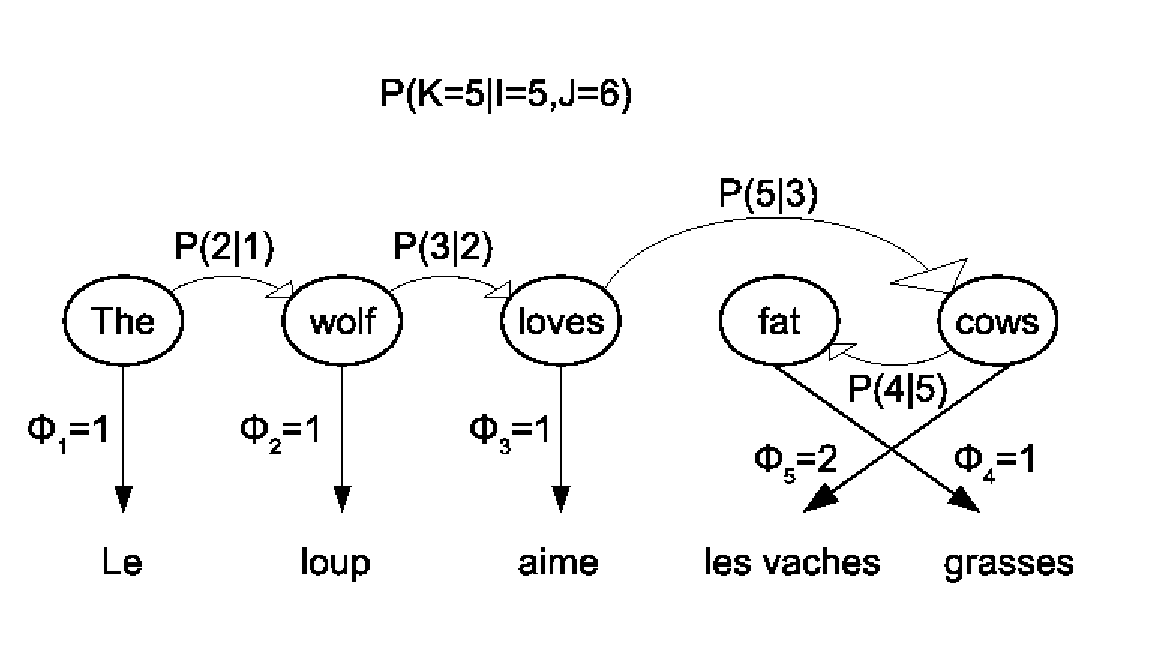
\includegraphics[scale=0.5]{figures/wordtophrase2.eps}
  \end{center}
  \caption{Illustrative example of an HMM word-to-phrase alignment model. The adjective noun sequence ``fat cows'' is
    reordered into the noun adjective sequence ``vaches grasses''. The word ``cows'' has fertility 2 as it is translated
    into the target phrase ``les vaches''.}
  \label{fig:wordtophrase}
\end{figure}
%
For example, if we use unigram probabilities, then we generate ``les vaches''
from ``cows'' according to
$P(\mbox{les vaches} \mid \mbox{cows}) = P(\mbox{les} \mid \mbox{cows}) P(\mbox{vaches} \mid \mbox{cows})$.
If we use bigram probabilities, then we generate ``les vaches'' from ``cows''
according to {\small $P(\mbox{les vaches} \mid \mbox{cows}) = P(\mbox{les} \mid \mbox{cows}) P(\mbox{vaches} \mid \mbox{cows},\mbox{les})$}.
Thus bigram probabilities take into account the context of the target word to
some extent.

\section{Log-Linear Model of Machine Translation}
\label{sec:loglinearModel}

%notes on adam berger paper
%model conditional prob
%p(y | x): x is phrase containing word "in", y is translation of "in"
%collect stats ptilda(x, y)
%binary feature: f(x, y) = 1 if y = en and April follows in
%expected value of f: ptilda(f) = sum_x,y ptilda(x,y) f(x,y)
%p(f) = sum_x,y ptilda(x) p(y | x) f(x,y)
%constraint: p(f) = ptilda(f)
%max entropy principle: choose p that satisfies the constraints
%and that maximizes entropy
%H(p) = -sum_x,y ptilda(x) p(y|x) log p(y|x)
%use Lagrange multiplier and Kuhn Tucker theorem to find that the solution
%is p(y|x) propto exp(\sum lambda_i f_i(x,y)). find lambda by max dual problem.
%also: p that satisfies constr and max entropy is also the
%p in the parametric family ... that maximizes likelihood of training sample.
%application to Candide.
%use max entropy modelling to predict translation of word in context.
%use max entropy modelling to predict word order.
%use max entropy modelling to segment.
%context dependent translation:
%first viterbi align training. then create events (x,y) (6 words
%surrounding in)
%incorporate this context dep translation into general translation model.

As we have seen in \autoref{sec:sourceChannelModel}, SMT was historically
framed as a source channel model.
\cite{berger-dellapietra-dellapietra:1996:CL} introduce maximum entropy
models for natural language processing. They show how a maximum entropy
model can be parameterized as an exponential, or log-linear model. They
apply this model to three machine translation related task. First, they
use a maximum entropy model to predict the translation of a word using
the context for that word. Then, they use a maximum entropy model to
predict the target language word order. Finally, they apply maximum
entropy modelling in order to predict the source sentence segmentation.

%notes och and ney 2002
%search done by the maximum approximation
%first present log linear model
%log linear model generalization of source channel model
%log linear model presented with additional alignment variable
%p(e_1^I, a_1^J | f_1^J) propto exp(sum_1^M lambda_m h_m(e_1^I, f_1^J, a_1^J))
%alignment template model
%p(f_1^J | e_1^I) = sum_{z_1^K, a_1^K} p(a_1^K | e_1^I) . p(z_1^K | a_1^K, e_1^I) . p(f_1^J | z_1^K, a_1^K, e_1^I)
%each component modeled with max entropy model

\citet{och-tillmann-ney:1999:EMNLP} notice that using an erroneous
version of the source channel model, that is using the following equation:
%
\begin{equation}
  \hat{\bm{e}} = \argmax_{\bm{e}} p(\bm{e} \mid \bm{f}) p(\bm{e})
\end{equation}
%
give comparable performance with respect to using the correct
formulation of the source channel model given in \autoref{eq:noisy}. In addition, it
allows them to use a dynamic programming algorithm for decoding.
\citet{och-ney:2002:ACL} propose the following extension:
%
\begin{align}
  \hat{\bm{e}} &= \argmax_{\bm{e}} p(\bm{e} \mid \bm{f}) \nonumber \\
               &= \argmax_{\bm{e}} \frac{\exp(\sum_{m=1}^M \lambda_m h_m(\bm{e}, \bm{f}))}{\sum_{\bm{e'}}\exp(\sum_{m=1}^M \lambda_m h_m(\bm{e'}, \bm{f}))} \nonumber \\
               &= \argmax_{\bm{e}} \exp(\sum_{m=1}^M \lambda_m h_m(\bm{e}, \bm{f})) \label{eq:loglinearModel}
\end{align}
%
where $h_m$ are called \emph{feature functions} and $\lambda_m$
are called \emph{feature weights}. The log-linear model is an extension
to the noisy channel model because it can be reduced to the original
noisy channel model with the following settings:
%
    \begin{itemize}
      \item $M = 2$
      \item $h_1({\bf e}, {\bf f}) = \log (p({\bf f}|{\bf e}))$
      \item $h_2({\bf e}, {\bf f}) = \log (p({\bf e}))$
      \item $\lambda_1 = \lambda_2 = 1$
    \end{itemize}
%
Log-linear models were originally trained with the maximum likelihood
criterion, which precisely makes them equivalent to maximum entropy
models~\citep{berger-dellapietra-dellapietra:1996:CL}. However,
more effective training techniques such as minimum error
training~\citep{och:2003:ACL} were introduced later on, that do
not require the computation of the normalization constant.
Thus, SMT are effectively simply linear models, with the objective
function presented in \autoref{eq:linearModel}:
%
\begin{equation}
  \hat{\bm{e}} = \argmax_{\bm{e}} \sum_{m=1}^M \lambda_m h_m(\bm{e}, \bm{f})
  \label{eq:linearModel}
\end{equation}

%In practice, \citet{och-ney:2002:ACL} do not use \autoref{eq:loglinearModel}.
%They introduce several latent variables in a so called \emph{alignment template}
%approach. The translation model is defined in \autoref{eq:alignmentTemplate}:
%
%\begin{equation}
%  p(e_1^I \mid f_1^J) = \sum_{z_1^K, a_1^K} p(a_1^K \mid e_1^I) p(z_1^K \mid a_1^K, e_1^I) p(f_1^J \mid z_1^K, a_1^K, e_1^I)
%  \label{eq:alignmentTemplate}
%\end{equation}
%
% TODO check if it is "correct" to invert the notation in above equation wrt to original publication
%where the variables $z_1^K$ and $a_1^K$ are alignment templates and the alignment of alignment templates.
%Each term in \autoref{eq:alignmentTemplate} is modelled as a maximum entropy model and search
%is carried out using the maximum approximation defined in \autoref{eq:maxApproximation}:
%
% TODO finish this
%\begin{align}
%  \hat{e_1^I} &= \argmax_{z_1}
%  \label{eq:maxApproximation}
%\end{align}

% TODO talk about training methods: GIS vs MERT

\section{Phrase Based Translation}
\label{sec:phraseBasedTranslation}

%notes on och et al 1999
%compare word based and phrase based
%e = argmax p(e) p(f|e)
%word based model: each source word (french) assigned exactly one target word (english)
%difficult to model context and also to translate compound words
%model two alignment levels: phrase level alignment between phrases and word level alignment between words within phrases
%word based approach: use an HMM
%p(f_1^J | e_1^I) = sum_{a_1^J} prod_j p(a_j | a_{j - 1}) p(f_j | e_{a_j})
%some restrictions are used (so called monotonicity): alignment jump between a_{j - 1} and a_j can only be 0, 1, 2.
%Q_{e'}(j, e): probability of best partial hypothesis (e_1^i, a_1^j) with e_i = e, e_{i - 1} = e' and a_j = i
%search: mapping j -> (a_j, e_{a_j})
%DP recursion:
%Q_e'(j, e) = p(f_j | e) . max {
%  p(0) . Q_e'(j - 1, e),
%  p(1) . max_e'' {p(e | e', e'') Q_e''(j - 1, e')},
%  p(2) . max_{e'', e'''} {p(e | e', e'') . p(e' | e'', e''') . Q_e'''(j - 1, e'')}
%  }
%optimal translation: max_e',e Q_e'(J, e) . p(\$ | e, e')
%extension to one-to-many alignment model.
%solution: reverse translation direction, then extend English vocab with multiple words, then redo standard training for original translation direction.
%alignment template approach
%problem with word based models: only allow one to many or many to one, or many to many but hacky solution
%model phrase to phrase is a way to model context.
%alignment template z: triple (Ftilda, Etilda, Atilda) alignment Atilda between source class sequence Ftilda and
%target class sequence Etilda.
%Atilda: matrix with binary values
%Atilda allows for many to many
%Ftilda and Etilda automatically trained bilingual classes
%use classes for better generalization
%alignment template applicable to sequence source words ftilda if
%alignment template classes and classes of source words are equal
%application of alignment template contraints the target words to have the right classes
%selection target words: p(etilda | z, ftilda)
%p(ftilda | (Ftilda, Etilda, Atilda), etilda) = delta(classes(etilda), Etilda) delta(classes(ftilda), Ftilda) prod_{j=1}^J (I???) p(f_j | Atilda, etilda)
%p(f_j | Atilda, etilda) = sum_{i = 0}^I p(i | j; Atilda) p(f_j | e_i)
%p(i | j, Atilda) = Atilda(i, j) / (sum_i Atilda(i, j))
%rien compris
%phrase level alignment
%decompose f_1^J and e_1^I into sequence of phrases
%f_1^J = ftilda_1^K
%assume that there is only one possible segmentation (possibly one of the differences between Och and Koehn)
%p(f_1^J | e_1^I) = p(ftilda_1^K | etilda_1^K)
%                 = sum_{atilda_1^K} p(atilda_1^K, ftilda_1^K | etilda_1^K)
%                 = sum_{atilda_1^K} p(atilda_1^K | etilda_1^K) p(ftilda_1^K | atilda_1^K, etilda_1^K)
%                 = sum_{atilda_1^K} prod_{k = 1}^K p(atilda_k | atilda_1^{k-1}, K) p(ftilda_k | etilda_{atilda_k})
%p(ftilda | etilda) = sum_z p(z| etilda) p(ftilda | z, etilda)
%training: s2t and t2s hmm without the max approximation
%get the viterbi alignments a_1^J and b_1^I
%use the grow diag symmetrisation heuristic.
%estimate bilingual word lexicon p(f|e): n_A(f, e) | n(e)
%train world classes
%extract consistent phrase pairs from alignment
%obtain n(z) of how often alignment template occurs in aligned corpus.
%relative freq estimate: p(z = (Ftilda, Etilda, Atilda) | etilda) = n(z) . delta(classes(etilda), Etilda) / n(classes(etilda))
%decoding search
%objective: argmax_{e_1^I} p(e_1^I p(e_1^I | f_1^J)) (wrong version of source channel model)
%use class-based 5g lm
%preprocessing before translation: filter alignment templates per source sentence, segment source sentence
%segmentation objective: argmax_{ftilda_1...ftilda_k = f_1^J} prod_{k=1}^K max_z p(z | ftilda_k)
%search: produce partial hypotheses with info: last target word, language model state,
%source coverage, last alignment template, position of last target word in alignment template
%instantiation (???), cost so far, backpointer
%integrate future cost because compare hypotheses that cover different parts of the input

%notes on och-ney 2004 (journal paper version of och et al. 1999)
%overview: align, extract, extracted phrases with alignment and word classes are
%called alignment templates
%log-linear model: hat{e_1^I} = argmax_{e_1^I} p(e_1^I | f_1^J)
%                             = argmax exp(sum_m=1^M lambda_m h_m(e_1^I, f_1^J))/Z
%parameters lambda trained with MLE (same as maximum entropy)
%or trained with MERT
%use latent variable
%p(e_1^I, a_1^J | f_1^J) = (1/Z) . exp(sum_1^M lambda_m h_m(e_1^I, f_1^J, a_1^J))
%description of word alignments etc.
%description of symmetrisation heuristics etc.
%symmetrized Viterbi alignments used to compute translation lexicon
%description of phrase-extract
%alignment templates: replace words with word classes and store
%alignment info for each phrase pair
%alignment template z = (F_1^J', E_1^I', Atilda)
%F_1^J' source class sequence
%E_1^I' target class sequence
%Atilda: alignment between source class seq and target class seq
%automatically train bilingual classes
%notation: etilda, ftilda target and source phrases
%p(z = (F_1^J', E_1^I', Atilda) | ftilda) = N(z) . delta(F_1^J', C(ftilda)) / N(C(ftilda%))
%remove alignment templates with prob less than 0.01
%limit on source phrase: between 4 and 7
%translation model
%f_1^J = ftilda_1^K
%e_1^I = etilda_1^K
%model described for a specific segmentation but in search
%optimal segmentation also searched for
%pi_1^K: permutation of the phrases, models phrase reordering
%etilda_k is translation of ftilda_{pi_k}
%alignment template between f_{pi_k} and e_k: z_k
%hidden variables in the model: pi_1^K, z_1^K
%use log-linear model, feature functions depend on source, target and hidden variables
%features
%alignment template selection
%h_AT(e_1^I, f_1^J, pi_1^K, z_1^K) = log prod_1^K p(z_k | f_{j_{pi_k - 1} + 1}^{j_{pi_k}%})
%h_WRD(e_1^I, f_1^J, pi_1^K, z_1^K) = log prod_1^I p(e_i | {f_j, (i,j) in A}, E_i)
%p(e_i | {f_j, (i,j) in A}, E_i)
%etc etc. hyper complique
%h_AL phrase alignment (reordering model)
%h_AL(e_1^I, f_1^J, pi_1^K, z_1^K) = sum_{k=1}^{K+1} |j_{pi_k - 1} - j_{pi_{k - 1}}
%3gram lm + 5g class based lm
%training: blabla
%search
%breadth-first search with pruning: beam search
%search objective:
%hat{e_1^I} = argmax_{e_1^I} sum_{pi_1^K, z_1^K} p(e_1^I, z_1^K, pi_1^K | f_1^J)
%           ~~ argmax_{e_1^I, pi_1^K, z_1^K} p(e_1^I, z_1^K, pi_1^K | f_1^J)
%           = argmax_{e_1^I, pi_1^K, z_1^K} sum_{m = 1}^M lambda_m h_m(e_1^I, f_1^J, pi_%1^K, z_1^K)
%use the max approximation
%structure of search space
%generate hypothesis left to right on the target
%preprocessing step: first determine all source phrases that match an alignment template
%unknown words carried over
%use 5-best target words for each target class according to some criterion
%use hypothesis recombination
%pruning done for hypotheses that cover the same number of source words
%future cost estimation
%rien compris
%exps etc. etc.

%notes on phrase-based mt by koehn's book
%EM training of phrase-based models: NO
%Extensions to the Reordering Model
%zh-en, ar-en, fr-en in contrast to de-en or jp-en
%lexicalized reordering
%reordering model p_o predicts orientation m,s,d given phrase pair f,e:
%p_o(orientation | f, e)
%extract each phrase pair with orientation type p_o(orientation | f, e) = count(orientation, e, f) / sum_o count(o, e, f)
%to be smoothed with prior p_o(orientation)
%phrase translation as classification: use max ent model to model context
%use phrase penalty to model source segmentation
%use word penalty to model length
%lexical weighting a la koehn
%used as smoothing for translation model
%lex(e|f, a) = prod_{i = 1}^length(e) (1/|{j | (i,j) in a}|) sum_{j | (i,j) in a} w(e_i | f_j)
%if english word unaligned, use the NULL word on the f side
%w estimated with rel freq from aligned corpus.
%use both lex(e|f,a) and lex(f|e,a)
%log linear model: TODO find out what's the objective in moses/koehn2003
%phrase-extract etc. etc.
%source channel phrase-based model:
%e = argmax p(f|e) p(e)
%  = argmax prod_i p(f_i | e_i) d(start_i - end_{i - 1} -1)
%justification: segmentations are equally likely, max approximation ??
%d(x) propto alpha^|x|

%notes on phrase-based mt decoding by koehn's book
%description of hypothesis expansion
%computational complexity: NP complete/hard
%hypothesis recombination
%simple example: [it] [is] vs. [it is]
%more complicated example: [he] [does not] vs. [it] [does not]
%note: instead of deleting the hyp, we still keep pointer
%so that we can output n-best
%stack decoding
%stack <-> number of foreign words translated
%problem: some hyps in a stack cover different regions of the input
%histogram pruning and threshold pruning
%reordering limit in search
%future cost or outside cost or rest cost
%cost of translation option: translation cost easy,
%language model cost approximated by lm without context,
%reordering model ignored
%for each translation option, compute the ``cost without context''
%then estimate the cheapest cost for translating any span in the
%input using DP
%use future cost in search: add the cost of the remaining (gappy) span
%to the partial cost

%notes on koehn et al 2003
%"Note that phrase translation with a lexical weight is a
%special case of the alignment template model [Och et al.,
%1999] with one word class for each word."

So far, we have presented two modelling approach to machine translation,
the original source channel model and the current log-linear model. We also
have presented word alignment, which was introduced in the source channel
model framework and which is a word based model.

% TODO motivation for phrase based: word based a:[1,J]->[1,I] so many to one mapping only
Phrase-based models were introduced as a practical solution to the
problem of translating words in context. Phrase-based models
currently achieve state-of-the-art performance. They can be defined
in the source channel model framework or the log-linear model framework.
Because the source channel model is rarely used anymore and because it is
a special case of a log-linear model, we will focus our presentation
on the log-linear model.

There are different variations on the phrase-based translation paradigm.
We will focus on two popular approaches, namely the alignment template
system~\citep{och-tillmann-ney:1999:EMNLP,och-ney:2004:CL} and the phrase-based
system~\citep{koehn-och-marcu:2003:NAACL,koehn:2010:book}.

\subsection{Alignment Template Phrase-Based Model}

The alignment template system uses a log-linear model presented
in \autoref{eq:loglinearModel} as a starting point and repeated in
\autoref{eq:loglinearModelRepeated}:
%
\begin{equation}
  \hat{\bm{e}} = \argmax_{e_1^J} \exp(\sum_{m = 1}^M \lambda_m h_m(f_1^J, e_1^I))
  \label{eq:loglinearModelRepeated}
\end{equation}
%
In order to reduce the number of parameters, the two latent variables $\pi_1^K$
and $z_1^K$ are introduced. $z_1^K$ is a sequence of \emph{alignment templates}
while $\pi_1^K$ is a permutation of size $K$. An alignment template
is a triple $(\tilde{F}, \tilde{E}, \tilde{A})$ where $\tilde{F}$ is a
sequence of source word classes, $\tilde{E}$ is a sequence of target
word classes and $\tilde{A}$ is an alignment between $\tilde{F}$
and $\tilde{E}$. $\pi_1^K$ together with $z_1^K$ define
a source segmentation of $f_1^J$ into source phrases $\tilde{f}_1^K$,
a target segmentation of $e_1^I$ into target phrases $\tilde{e}_1^K$ and
a bijective mapping between source phrases and target phrases where
$\tilde{f}_{\pi_k}$ is mapped to $\tilde{e}_{k}$ for $k \in [1,K]$.
The alignment templates $z_1^K$ are constrained in such a way that
the alignment template classes match the word classes.

Using the max approximation and making the feature
functions depend on the hidden variables, the translation model
can be rewritten in \autoref{eq:alignmentTemplateModel}:
%
\begin{equation}
  \hat{\bm{e}} = \argmax_{e_1^J, z_1^K, \pi_1^K} \exp(\sum_{m = 1}^M \lambda_m h_m(f_1^J, e_1^I, \pi_1^K, z_1^K))
  \label{eq:alignmentTemplateModel}
\end{equation}
%

\subsection{Standard Phrase-Based Model}

The standard phrase-based model is similar to the alignment template
model but does not make use of source and target word classes.
Again, we use the latent variables $\pi_1^K$ and $z_1^K$.
This time, $z_k$ is defined as a triple $(\tilde{f}, \tilde{e}, \tilde{A})$
where $\tilde{f}$ is a sequence of source words, $\tilde{e}$ is a sequence
of target words and $\tilde{A}$ is an alignment between $\tilde{f}$ and $\tilde{e}$.
The reason for using the alignment information between phrase pairs is to be able
to compute the lexical feature. Because the lexical feature can be computed
by other means than this alignment information, it is also possible to simply
define $z_k$ as a phrase pair.

We have presented two variants of the phrase-based model. We will now
describe how to obtain the phrase pairs used for the latent variable $z$.

\subsection{Symmetrisation Heuristics}
\label{sec:symmetrisationHeuristics}

A preliminary step to phrase pair extraction is to symmetrize alignments.
As noted in \autoref{sec:StatisticalMachineTranslationWordAlignment}, alignment
models are not symmetric as they only allow many-to-one mapping from source to
target. \citet{och-tillmann-ney:1999:EMNLP} designed
a heuristic to symmetrise alignments trained in both source to target
and target to source directions. \citet{koehn-och-marcu:2003:NAACL}
later extend the set of heuristics and examine the impact on translation
performance for each heuristic.

Let us consider a sentence pair $(\bm{f}, \bm{e})$,
an alignment
from $\bm{e}$ to $\bm{f}$, $\bm{a_{e2f}}$, and an alignment from $\bm{f}$ to
$\bm{e}$, $\bm{a_{f2e}}$. Different symmetrisation heuristics that result in a
symmetric alignment $\bm{a}$ are defined as follows:
%
\begin{itemize}
  \item \emph{Union}: $\bm{a} = \bm{a_{e2f}} \cup \bm{a_{f2e}}$
  \item \emph{Intersection}: $\bm{a} = \bm{a_{e2f}} \cap \bm{a_{f2e}}$
  \item \emph{Grow-diag} (grow diagonal): $\bm{a} = (\bm{a_{e2f}} \cap \bm{a_{f2e}}) \cup GD$. $GD$ is the set of
    alignment links that are in the union and not in the intersection, whose words are not already aligned and
    that are neighbours of alignment links in the intersection.
\end{itemize}
%
%Symmetrised alignments have be shown to produce better translation results than
%unidirectional alignments. However, we find in one of our experiments that this
%is not always the case (see \autoref{sec:extractionFromPosteriorsSymmetrising}).

% This should review phrase based SMT.
% Why: the gyro decoder is like a phrase based SMT decoder.

% phrase based extraction + stack base decoding

\subsection{Phrase Pair Extraction}
\label{sec:phrasextract}

Grammar rules are extracted from symmetrised alignments.
Let us consider a sentence pair $(\bm{f},\bm{e})$ and an alignment $\bm{a}$.
We extract all phrase pairs that are {\em consistent} with the alignment.
This means that we extract all phrase pairs $(f_{j_1}^{j_2},e_{i_1}^{i_2})$ that
satisfy \autoref{eq:consistent} and \autoref{eq:atLeastOneLink}:
%
\begin{align}
  & \forall (j,i) \in \bm{a}, (j \in [j_1, j_2] \Leftrightarrow i \in [i_1,i_2]) \label{eq:consistent} \\
  & [j_1, j_2] \times [i_1, i_2] \cap \bm{a} \neq \emptyset \label{eq:atLeastOneLink}
\end{align}
%
%TODO better example
\autoref{eq:consistent} requires that no alignment link be between a word
inside the phrase pair and a word outside the phrase pair.
\autoref{eq:atLeastOneLink} requires that there be at least one alignment link
between a source word in the source phrase and a target word in the target phrase.
For example, in Figure \ref{fig:ruleextract}, the phrase pair
(Buenas tardes, Good afternoon) is extracted while the
phrase pair (tardes !, !) is not because the word ``tardes'' is aligned
outside the phrase pair.
%
      \begin{figure}[h]
        \begin{center}
          \vspace*{-5cm}
          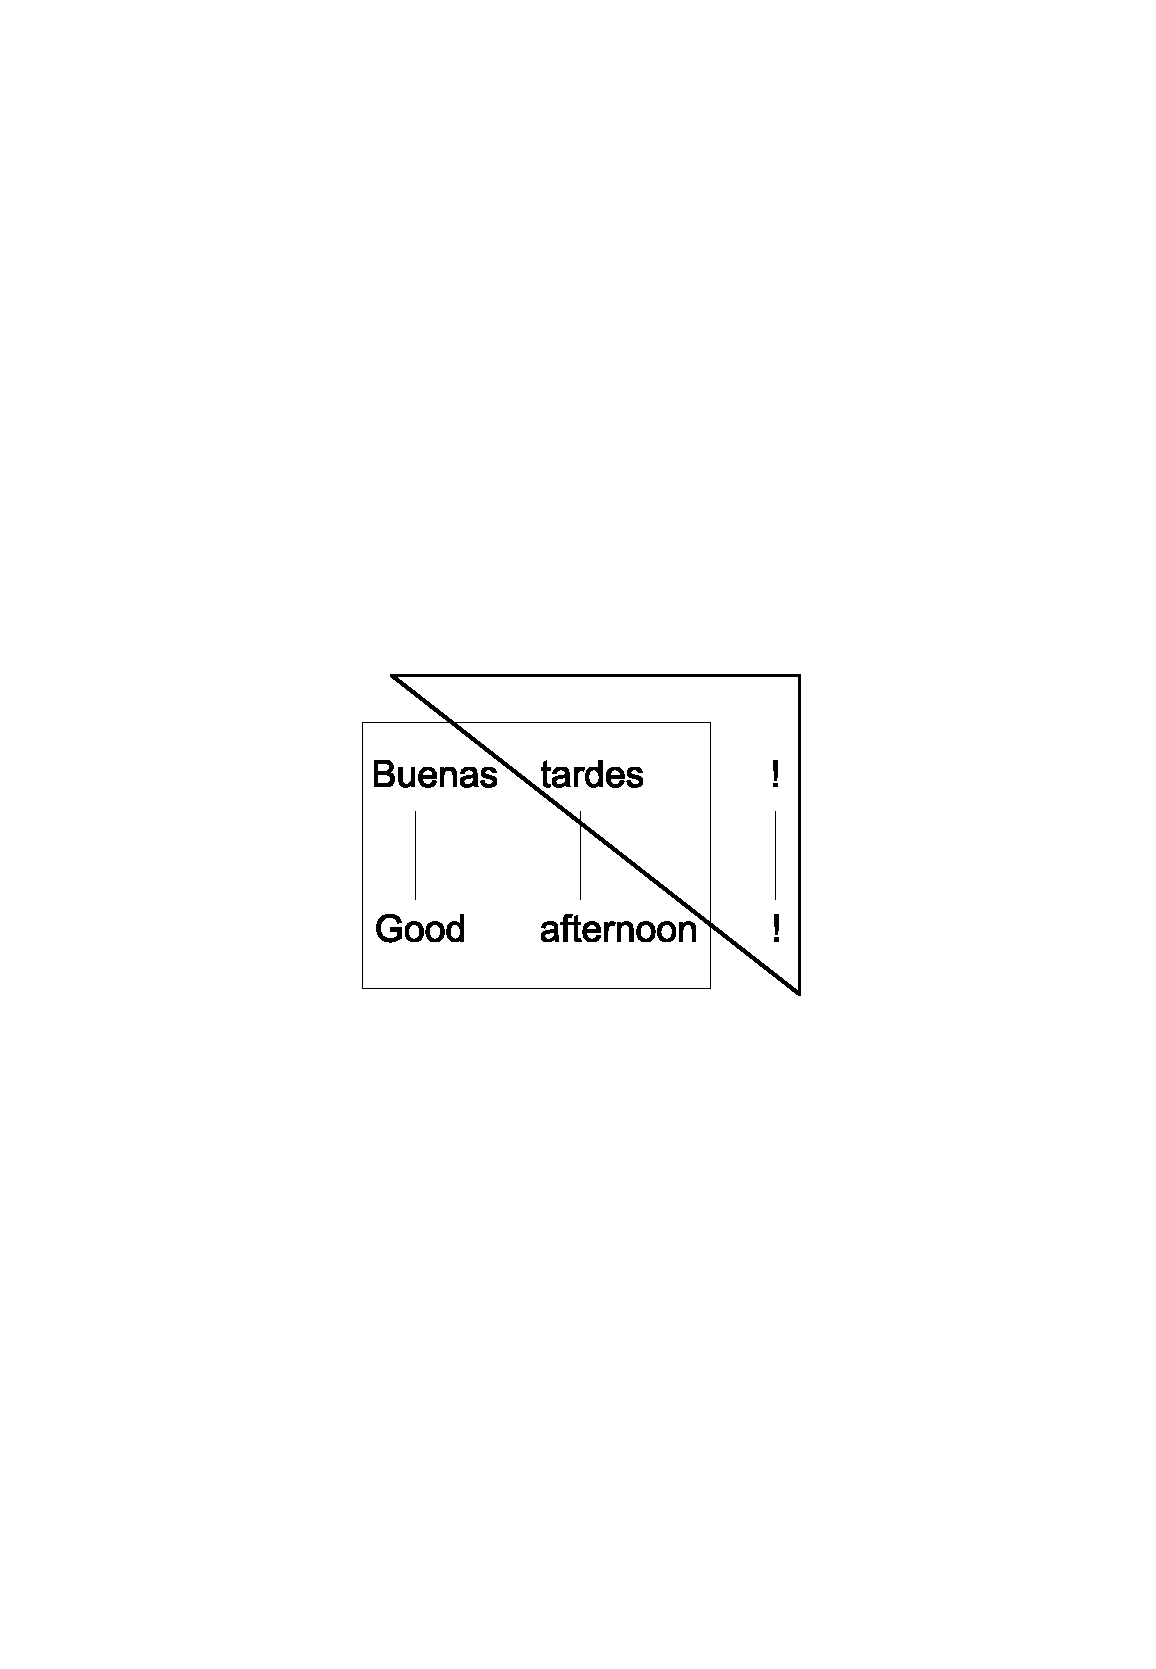
\includegraphics[scale=0.5]{figures/phraseextraction.eps}
          \vspace*{-5cm}
        \end{center}
        \caption{Rule extraction for a sentence pair. For example, the phrase (Good afternoon, Buenas tardes) is extracted. The phrase pair (tardes !, !) is not extracted because it is
        not consistent with the alignment.}
        \label{fig:ruleextract}
      \end{figure}

\subsection{Phrase Based Decoding}

%notes on knight 1999 NP complete
%blabla on cryptograph and pos tagging
%machine translation
%v total English words
%bigram source model with v^2 parameters
%substitution/permutation channel models
%parallel corpus (sentence length <= m)
%monolingual french (???) sentence (length <= m)
%e_i has fertility phi_i: parameter n(phi | e)
%french words produced according to s(f|e) and permuted according to d(j|i,m,l)
%model 1 EM training
%collect estimate epsilon(m | l) from data
%set s(f|e) uniform initially
%basically, decoding with M1 is NP-complete
%reduction from hamilton circuit

We can now present the decoding process in phrase based translation.
We will first introduce the translation process. Then, we will
describe how translation hypotheses are built incrementally.
We will then motivate the need for pruning and how pruning
is carried out. Finally, we will describe how future cost estimation
may reduce search errors.

\paragraph{Translation Process}

Given a source sentence, the translation process is to iteratively
pick a source phrase, translate that source phrase into a target phrase
and append the target phrase to the translation, until the source
sentence has been entirely covered by source phrases. While the process is not
complete, the concatenation of target phrases is called a
\emph{partial hypothesis}.

\paragraph{Hypothesis Expansion}

The decoding process starts from an initial empty partial hypothesis.
This empty partial hypothesis is extended by picking source phrases,
appending their translations to the empty hypothesis.
At this stage, we have obtained several partial hypotheses.
The partial hypotheses are repeatedly extended until
all source words have been covered.
Partial hypotheses are represented by states
that contain the information necessary to
compute the cost of an extension.
If we use an $n$-gram language model as a feature,
the state will encode the cost of the partial hypothesis
and the last $n - 1$ words of the partial hypothesis.

\paragraph{Hypothesis Recombination}

When two partial hypothesis share the same $n - 1$
words, only the partial hypothesis with the lower
cost can lead to the best final hypothesis. Therefore,
the partial hypothesis with higher cost can be discarded, or
alternatively, it is possible to make these two partial
hypotheses share the same state for rescoring purposes.

\paragraph{Stack Based Decoding and Pruning}

The decoding search space is very large: given a source sentence of size
$J$, the translation process has to pick one of $2^J$ possible segmentation
in order to obtain a source phrase sequence, then pick a permutation
for that source phrase sequence and finally pick a translation for each
phrase. Therefore, a decoder has to make approximations.

The partial hypotheses mentioned above are grouped in \emph{stacks}
by the number of source words covered.
This allows pruning. Each time a hypothesis expansion produces a hypothesis that
belongs to a certain stack, that stack is pruned.
There are two types of pruning, histogram pruning and threshold
pruning. Histogram pruning enforces a maximum number
of partial hypotheses in each stack. Threshold pruning
examines the cost of the best partial hypothesis in a stack
and discards all partial hypotheses in that stack whose cost
is greater than the best cost plus a threshold.

\paragraph{Future Cost}

Partial hypotheses that cover the same number of source
words are grouped together for pruning purposes. However,
their cost may not be directly comparable, for example
partial hypotheses that correspond to the translation of frequent
words in the source might have a smaller cost than partial hypotheses
that correspond to the translation of rare words in the source.
To address this issue, a future cost that represents how difficult it is
to translate the rest of the sentence is added to the model cost of each
partial hypothesis.

\section{Hierarchical Phrase-Based Translation}
\label{sec:hierarchicalPhraseBasedTranslation}

  \subsection{Introduction and Motivation} \label{sec:hierintro}

  Hierarchical phrase-based translation (hierarchical translation in short) was shown to
  outperform state-of-the-art phrase-based systems~\citep{chiang:2005:ACL,chiang:2007:CL}.
  Hierarchical translation relies on the hierarchical grammar formalism defined in Section \ref{sec:hiergrammar}. A closely related formalism, inversion
  transduction grammars, was previously introduced~\citep{wu:1995:IJCAI,wu:1997:CL}. The motivation for this type
  of formalism is to allow nested reordering which can happen between language pairs with very different word order such as 
  Chinese and English. For example, the Chinese sentence with English gloss in \autoref{fig:example} requires nested reordering~\citep{chiang:2007:CL}.


  \begin{figure}
    \begin{center}
      \begin{footnotesize}
      %\begin{tabular}{*{11}{l}}
      \begin{tabular}{p{0.9cm} p{1cm} p{0.2cm} p{0.3cm} p{1.9cm} p{0.3cm} p{1.5cm} p{0.3cm} p{0.9cm} p{1cm} p{0.9cm}}
%        \textbf{Chinese} & 澳洲 & 是 & 与 & 北韩 & 有 & 邦交 & 的 & 少数 & 国家 & 之一 \\
        \textbf{Pinyin}  & Aozhou & shi & yu & Beihan & you & bangjiao & de & shaoshu & guojia & zhiyi \\
        \textbf{Gloss} & Australia & is & with & North Korea & have & dipl. rel. & that & few & countries & one of \\
         & & & & & & & & & & \\
        \textbf{English} & \multicolumn{10}{l}{Australia is one of the few countries that have diplomatic relations with North Korea} \\
      \end{tabular}
      \end{footnotesize}
    \end{center}
    \caption{Example of Chinese sentence that needs nested reordering to be translated into English.}
    \label{fig:example}
  \end{figure}

  
%  \begin{figure}
%    \begin{center}
%      \includegraphics[width=13cm]{figures/example.ps}
%    \end{center}
%    \caption{Example of Chinese sentence with English gloss that needs nested reordering to be translated into English}
%    \label{fig:example}
%  \end{figure}
  

  \begin{itemize}
    \item ``with North Korea have diplomatic relations'' must be reordered into 
      ``have diplomatic relations with North Korea''.
    \item ``few countries one of'' must be reordered into ``one of (the) few countries''.
    \item After the two previous segments are reordered, ``have diplomatic relations with North Korea that one of the few countries'' must be reordered into ``one of the few countries that have diplomatic relations with North Korea''.
  \end{itemize}
%
  Phrase-based systems can model this type of movement but they need to use very long phrase pairs, which is
  impractical because of data sparsity. On the other hand, hierarchical grammars do model this type of movement using
  shorter phrase pairs.

  \subsection{Hierarchical Grammar} \label{sec:hiergrammar}

  A hierarchical grammar, which is a particular instance of a synchronous context free grammar is a set of rewrite rules of the following type:

  \begin{equation}
    X \rightarrow \langle \gamma, \alpha, \sim \rangle \nonumber
  \end{equation}

  \noindent where $X$ is a nonterminal, $\gamma$ and $\alpha$ are sequences of terminals and nonterminals and $\sim$ is an alignment
  between nonterminals. Terminals that appear in $\gamma$ are words in the source language while terminals that appear in $\alpha$ are
  words in the target language. Nonterminals are chosen from a finite set disjoint from the set of terminals. The alignment between nonterminals
  indicates which nonterminals in the source and target languages correspond to each other. The alignment $\sim$ can be written with 
  a set of matching indices.

  A hierarchical grammar also usually contains the following rules called glue rules:

  \begin{eqnarray}
    S &\rightarrow& \langle X, X \rangle \nonumber \\
    S &\rightarrow& \langle S X, S X \rangle \nonumber
  \end{eqnarray}

  \noindent with $S$ the start symbol. The first glue rule is necessary to be able to start a derivation.
  The second glue rule allows concatenation of phrases or rules.

  Let us consider for example the following grammar~\citep{chiang:2007:CL} where each rewrite rule is given a name $R_i$:

  \begin{eqnarray}
    R_1&:& S \rightarrow \langle X, X \rangle \nonumber \\
    R_2&:& S \rightarrow \langle S X, S X \rangle \nonumber \\
    R_3&:& X \rightarrow \langle X_1 \mbox{ de } X_2, \mbox{ the } X_2 \mbox{ that } X_1 \rangle \nonumber \\
    R_4&:& X \rightarrow \langle X \mbox{ zhiyi}, \mbox{ one of } X \rangle \nonumber \\
    R_5&:& X \rightarrow \langle \mbox{yu } X_1 \mbox{ you } X_2, \mbox{ have } X_2 \mbox{ with } X_1 \rangle \nonumber \\
    R_6&:& X \rightarrow \langle \mbox{Aozhou}, \mbox{ Australia} \rangle \nonumber \\
    R_7&:& X \rightarrow \langle \mbox{shi}, \mbox{ is} \rangle \nonumber \\
    R_8&:& X \rightarrow \langle \mbox{Beihan}, \mbox{ North Korea} \rangle \nonumber \\
    R_9&:& X \rightarrow \langle \mbox{bangjiao}, \mbox{ diplomatic relations} \rangle \nonumber \\
    R_{10}&:& X \rightarrow \langle \mbox{shaoshu guojia}, \mbox{ few countries} \rangle \nonumber
  \end{eqnarray}
%
  With this grammar, it is possible to write a derivation, that is a sequence of rules, that rewrites the start symbol $S$ into the sentence pair presented in Section \ref{sec:hierintro} \cite{chiang:2007:CL}. For example we can apply the derivation \linebreak $R_2,R_2,R_1,R_6,R_7,R_4,R_3,R_{10},R_5,R_9,R_8$ as
  follows:

  \begin{footnotesize}
  \begin{eqnarray}
    S &\rightarrow& \langle S X, S X \rangle \nonumber \\
      &\rightarrow& \langle S X_1 X_2, S X_1 X_2 \rangle \nonumber \\
      &\rightarrow& \langle X_1 X_2 X_3, X_1 X_2 X_3 \rangle \nonumber \\
      &\rightarrow& \langle \mbox{Aozhou } X_2 X_3, \mbox{Australia } X_2 X_3 \rangle \nonumber \\
      &\rightarrow& \langle \mbox{Aozhou shi } X_3, \mbox{Australia is } X_3 \rangle \nonumber \\
      &\rightarrow& \langle \mbox{Aozhou shi } X \mbox{ zhiyi}, \mbox{Australia is one of } X \rangle \nonumber \\
      &\rightarrow& \langle \mbox{Aozhou shi } X_1 \mbox{ de } X_2 \mbox{ zhiyi}, \mbox{Australia is one of the } X_2 \mbox{ that } X_1 \rangle \nonumber \\
      &\rightarrow& \langle \mbox{Aozhou shi } X_1 \mbox{ de shaoshu guojia zhiyi}, \mbox{Australia is one of the few countries that } X_1 \rangle \nonumber \\
      &\rightarrow& \langle \mbox{Aozhou shi yu } X_1 \mbox{ you } X_2 \mbox{ de shaoshu guojia zhiyi}, \nonumber \\
      &&                    \mbox{Australia is one of the few countries that have } X_2 \mbox{ with } X_1 \rangle \nonumber \\
      &\rightarrow& \langle \mbox{Aozhou shi yu } X_1 \mbox{ you bangjiao de shaoshu guojia zhiyi}, \nonumber \\
      &&                    \mbox{Australia is one of the few countries that have diplomatic relations with } X_1 \rangle \nonumber \\
      &\rightarrow& \langle \mbox{Aozhou shi yu Beihan you bangjiao de shaoshu guojia zhiyi}, \nonumber \\ 
      &&                    \mbox{Australia is one of the few countries that have diplomatic relations with North Korea} \rangle \nonumber
  \end{eqnarray}
  \end{footnotesize}
%
  The definition given for a hierarchical grammar is very general. In practice, systems impose constraints on the types of rule the grammar contains
  for efficiency reasons.
  Before describing an example of constraints, we first need to define the notion of rule pattern \cite{iglesias-degispert-banga-byrne:2009:EACL}. Let $w$ denote a sequence
  of terminals. Given a grammar rule, we define its pattern by its right hand side where terminal sequences have been replaced by $w$.
  For example, the pattern for the rule $ X \rightarrow \langle \mbox{ Buenas tardes } X, \mbox{Good afternoon } X \rangle$ is $\langle w X, w X \rangle$.
  \citet{chiang:2007:CL} defines the following set of pattern-related constraints which rules in a hierarchical grammar must satisfy:
%
  \begin{itemize}
    \item If a rule has a pattern $\langle w, w \rangle$, then $|w| < 10$. This corresponds to the maximum phrase length. We call this type of rule a {\em phrasal rule}. Similarly, if a rule contains
      a nonterminal on its right hand side, we call it a {\em hierarchical rule}.
    \item A rule $X \rightarrow \langle \gamma, \alpha \rangle$ must satisfy $|\gamma| \leq 5$.
    \item Rules have at most 2 nonterminals.
    \item The source side of a rule cannot have adjacent nonterminals. \citet{setiawan-resnik:2010:NAACL} relax this constraint. Note that the target side can have adjacent nonterminals. %, for example see Section \ref{sec:emnlp10gramdef}.
  \end{itemize}
%
  More fine-grained constraints can be defined on patterns. For example, our current baseline system uses the configuration in Table \ref{tab:patternconfig}
  for its grammar. This grammar was obtained following a greedy strategy of adding in turn most beneficial patterns for Arabic-English translation.

  \begin{table}[htbp]
    \begin{center}
      \footnotesize
      \begin{tabular}{|r@{ , }l|c||r@{ , }l|c|} \hline 
        {\bf \SR[source]} & {\bf\TR[target]} & {\bf include} & {\bf \SR[source]} & {\bf\TR[target]} & {\bf include} \\ \hline
        \SR[$w~X$] & \TR[$w~X$] & \red{no}  & \SR[$X~w$] & \TR[$w~X$] & yes \\
        \SR[$w~X$] & \TR[$X~w$] & yes &  \SR[$X~w$] & \TR[$w~X~w$] & yes \\
        \SR[$w~X$] & \TR[$w~X~w$] & yes  & \SR[$X~w$] & \TR[$X~w$] & \red{no} \\
        \hline
        \SR[$w~X~w$] & \TR[$w~X$] & yes &  \SR[$w~X~w$] & \TR[$X~w$] & yes \\
        \SR[$w~X~w$] & \TR[$w~X~w$] & yes &  \multicolumn{2}{|c|}{} & \\
        \hline
        \SR[$X1~w~X2$] & \TR[$w~X1~w~X2$] & \red{no} &  \SR[$X2~w~X1$] & \TR[$w~X1~w~X2$] & yes \\
        \SR[$X1~w~X2$] & \TR[$w~X1~w~X2~w$] & \red{no} &  \SR[$X2~w~X1$] & \TR[$w~X1~w~X2~w$] & yes \\
        \SR[$X1~w~X2$] & \TR[$w~X1~X2$] & \red{no} & \SR[$X2~w~X1$] & \TR[$w~X1~X2$] & yes \\
        \SR[$X1~w~X2$] & \TR[$w~X1~X2~w$] & \red{no} & \SR[$X2~w~X1$] & \TR[$w~X1~X2~w$] & yes \\
        \SR[$X1~w~X2$] & \TR[$X1~w~X2$] & \red{no} & \SR[$X2~w~X1$] & \TR[$X1~w~X2$] & yes \\
        \SR[$X1~w~X2$] & \TR[$X1~w~X2~w$] & \red{no} & \SR[$X2~w~X1$] & \TR[$X1~w~X2~w$] & yes \\
        \SR[$X1~w~X2$] & \TR[$X1~X2~w$] & \red{no} & \SR[$X2~w~X1$] & \TR[$X1~X2~w$] & yes \\
        \hline
        \SR[$w~X1~w~X2$] & \TR[$w~X1~w~X2$] & \red{no} & \SR[$w~X2~w~X1$] & \TR[$w~X1~w~X2$] & yes \\
        \SR[$w~X1~w~X2$] & \TR[$w~X1~w~X2~w$] & yes & \SR[$w~X2~w~X1$] & \TR[$w~X1~w~X2~w$] & yes \\
        \SR[$w~X1~w~X2$] & \TR[$w~X1~X2$] & yes & \SR[$w~X2~w~X1$] & \TR[$w~X1~X2$] & yes \\
        \SR[$w~X1~w~X2$] & \TR[$w~X1~X2~w$] & yes & \SR[$w~X2~w~X1$] & \TR[$w~X1~X2~w$] & yes \\
        \SR[$w~X1~w~X2$] & \TR[$X1~w~X2$] & yes & \SR[$w~X2~w~X1$] & \TR[$X1~w~X2$] & yes \\
        \SR[$w~X1~w~X2$] & \TR[$X1~w~X2~w$] & yes & \SR[$w~X2~w~X1$] & \TR[$X1~w~X2~w$] & yes \\
        \SR[$w~X1~w~X2$] & \TR[$X1~X2~w$] & yes & \SR[$w~X2~w~X1$] & \TR[$X1~X2~w$] & yes \\
        \hline
        \SR[$X1~w~X2~w$] & \TR[$w~X1~w~X2$] & yes & \SR[$X2~w~X1~w$] & \TR[$w~X1~w~X2$] & yes \\
        \SR[$X1~w~X2~w$] & \TR[$w~X1~w~X2~w$] & yes & \SR[$X2~w~X1~w$] & \TR[$w~X1~w~X2~w$] & yes \\
        \SR[$X1~w~X2~w$] & \TR[$w~X1~X2$] & yes & \SR[$X2~w~X1~w$] & \TR[$w~X1~X2$] & yes \\
        \SR[$X1~w~X2~w$] & \TR[$w~X1~X2~w$] & yes & \SR[$X2~w~X1~w$] & \TR[$w~X1~X2~w$] & yes \\
        \SR[$X1~w~X2~w$] & \TR[$X1~w~X2$] & yes & \SR[$X2~w~X1~w$] & \TR[$X1~w~X2$] & yes \\
        \SR[$X1~w~X2~w$] & \TR[$X1~w~X2~w$] & \red{no} & \SR[$X2~w~X1~w$] & \TR[$X1~w~X2~w$] & yes \\
        \SR[$X1~w~X2~w$] & \TR[$X1~X2~w$] & yes & \SR[$X2~w~X1~w$] & \TR[$X1~X2~w$] & yes \\
        \hline
        \SR[$w~X1~w~X2~w$] & \TR[$w~X1~w~X2$] & \red{no} & \SR[$w~X2~w~X1~w$] & \TR[$w~X1~w~X2$] & yes \\
        \SR[$w~X1~w~X2~w$] & \TR[$w~X1~w~X2~w$] & \red{no} & \SR[$w~X2~w~X1~w$] & \TR[$w~X1~w~X2~w$] & yes \\
        \SR[$w~X1~w~X2~w$] & \TR[$w~X1~X2$] & \red{no} & \SR[$w~X2~w~X1~w$] & \TR[$w~X1~X2$] & yes \\
        \SR[$w~X1~w~X2~w$] & \TR[$w~X1~X2~w$] & \red{no} & \SR[$w~X2~w~X1~w$] & \TR[$w~X1~X2~w$] & yes \\
        \SR[$w~X1~w~X2~w$] & \TR[$X1~w~X2$] & \red{no} & \SR[$w~X2~w~X1~w$] & \TR[$X1~w~X2$] & yes \\
        \SR[$w~X1~w~X2~w$] & \TR[$X1~w~X2~w$] & \red{no} & \SR[$w~X2~w~X1~w$] & \TR[$X1~w~X2~w$] & yes \\
        \SR[$w~X1~w~X2~w$] & \TR[$X1~X2~w$] & \red{no} & \SR[$w~X2~w~X1~w$] & \TR[$X1~X2~w$] & yes \\
        \hline
      \end{tabular}
    \end{center}
    \caption{Rule patterns included in a baseline hierarchical grammar.}
    \label{tab:patternconfig}
  \end{table}
  
  Another restriction on hierarchical grammar is the amount of reordering allowed. \citet{degispert-iglesias-blackwood-banga-byrne:2010:CL} investigate the use
  of shallow-$N$ grammars that precisely control the depth of reordering in translation. We describe here 
  shallow-1 grammars~\citep{iglesias-degispert-banga-byrne:2009:EACL,degispert-iglesias-blackwood-banga-byrne:2010:CL} as
  they will be used for (TODO refer to ru-en WMT experiments). Shallow-1 grammars
  allow only one level of reordering, they do not allow nested reordering as in the example presented in Section \ref{sec:hierintro}. A shallow-1
  grammar is defined as following:
  
  \begin{align*}
    S &\rightarrow \langle X , X \rangle \\
    S &\rightarrow \langle S X , S X \rangle \\
    X &\rightarrow \langle \gamma_s , \alpha_s \rangle (\gamma_s, \alpha_s \in (T \cup \{V\})^{+}) \\
    X &\rightarrow \langle V , V \rangle \\
    V &\rightarrow \langle s , t \rangle (s \in T^{+}, t \in  T^{*})
  \end{align*}
  
  \noindent where $S$ is the start symbol, $T$ is the set of terminals and $V$ is the set of nonterminals. There are two nonterminals
  apart from the start symbol: $X$ and $V$. The rule type $X \rightarrow \langle \gamma_s , \alpha_s \rangle$ corresponds
  to all hierarchical rules. It is possible to apply this type of rule only once. Indeed, the
  right hand side contains only one type of nonterminal, $V$, which can be rewritten only with a phrasal rule corresponding
  to the line $V \rightarrow \langle s , t \rangle$. Note that for rules of the type $V \rightarrow \langle s , t \rangle$, $t$ can be
  the empty word, thus these rules, called {\em deletion rules}, allow deletion on the target side. Shallow-1 grammar are used for language pairs that do not present
  much reordering. Shallow-1 grammars were previously shown to work as well as full hierarchical grammars
  for the Arabic-English language pair~\citep{iglesias-degispert-banga-byrne:2009:EACL} and for
  the Spanish-English language pair~\citep{iglesias-degispert-banga-byrne:2009:SEPLN}.
  In addition, shallow-1 grammars reduce the search space of the decoder greatly, resulting in a much faster decoding
  time, a reduced memory use and potentially less search errors.

  % TODO log linear model for hpbt

    \subsection{Log-linear Model for Hierarchical Phrase-Based Translation} \label{sec:loglinear}

    We now define in more detail the log-linear model for hierarchical translation, which usually makes a maximum (max) approximation.
    For a sentence pair $(\bm{f}, \bm{e})$, let us define $\mathcal{D}$ the set of possible derivations $D$ of this sentence pair under 
    a hierarchical grammar. We will use the following notation for a derivation $D$:
    
    \begin{itemize}
%      \item $T$, the structure of the tree (that is the tree $D$ without leaves)
      \item the foreign yield $\bm{f}$. We define $f(D) = \bm{f}$
      \item the English yield $\bm{e}$. We define $e(D) = \bm{e}$
    \end{itemize}

    %Let us define $d = (T,{\bf f})$, so that we have $D = (d,{\bf e})$. 
    We can now derive the log-linear model for hierarchical translation:

    \begin{eqnarray}
      \hat{{\bf e}} &=& \argmax_{\bm{e}} p(\bm{e} \mid \bm{f}) \nonumber \\
                    &=& \argmax_{\bm{e}} \sum_{D \in \mathcal{D}} p(D,\bm{e} \mid \bm{f}) \mbox{ (marginalisation)} \nonumber \\
                    %&=& \argmax_{e} \sum_{d} p(d,{\bf e}|{\bf f}) \mbox{ (simply because the event D,{\bf e} is the same as the event d,{\bf e}} \\
                    &=& \argmax_{\bm{e}} \argmax_{D \in \mathcal{D}} p(D,\bm{e} \mid \bm{f}) \mbox{ (max approximation)} \nonumber \\
                    &=& e(\argmax_{{\bf e},D \in \mathcal{D}} p(D,{\bf e}|{\bf f})) \nonumber \\
                    &=& e(\argmax_{D | f(D) = {\bf f}} p(D))
    \end{eqnarray}

    Thanks to the max approximation, the distribution over derivations instead of the distribution over English
    sentences is modelled log-linearly and we obtain finally the following decoding equation:
%
    \begin{equation} \label{eq:decoding}
      \hat{{\bf e}} = e(\argmax_{D | f(D) = {\bf f}} \exp(\sum_{m=1}^M \lambda_m h_m(D)))
    \end{equation}
%
    One of the features, the language model, plays a particular role. The language model feature can be written as:
%    
    \begin{equation}
      h_M(D) = p_{LM}(e(D))
    \end{equation}
    
    \noindent where $M$ is the index of the language model feature, $p_{LM}$ is the language model and $e(D)$ is the English
    yield of the derivation $D$. It is not possible to compute the language model using dynamic programming since
    the language model needs context in order to be computed, therefore the language model feature is typically
    computed after a parsing step.
    
    Note that Equation (\ref{eq:decoding}) is an approximation and that there have been attempts to perform marginalisation over the latent variable 
    $D$ while keeping the translation process tractable~\citep{blunsom-cohn-osborne:2008:ACL}.

    %We now describe which features are used in our system, except for the language model which will be presented in Section \ref{lm}.

  \subsection{Rule Extraction} \label{sec:hierruleextract}

  We have so far given the definition of a hierarchical grammar and explained how it is used with statistical models.
  It is also necessary to extract an appropriate grammar, that is the rules it contains. The extraction
  is performed on a parallel corpus. The parallel corpus is first word-aligned, then
  rules are extracted from the alignment.

  We first extract phrase pairs as described in \autoref{sec:phrasextract}.
  For each extracted phrase pair $(f_{j_1}^{j_2}, e_{i_1}^{i_2})$,
  we define the following
  rule: $X \rightarrow \langle f_{j_1}^{j_2},e_{i_1}^{i_2} \rangle$.
  These rules are called {\em initial rules} or {\em phrasal rules}.
      We extend the set of initial rules with the following recursion: given a rule  $X \rightarrow \langle \gamma, \alpha \rangle$
      and an initial rule $X \rightarrow \langle f_{j_1}^{j_2},e_{i_1}^{i_2} \rangle$ such that $\gamma = \gamma_1 f_{j_1}^{j_2} \gamma_2$
      and $\alpha = \alpha_1 e_{i_1}^{i_2} \alpha_2$, then extract the rule $X \rightarrow \langle \gamma_1 X \gamma_2, \alpha_1 X \alpha_2 \rangle$.
      Note that $\gamma_1$ or $\gamma_2$, but not both, can be the empty word, and similarly for $\alpha_1$ and $\alpha_2$.

%      \subsubsection{Glue Rules}
%
%      The following two rules are added in order to respectively be able to start a derivation and to add concatenation capabilities to the grammar, as
%      mentioned in Section \ref{sec:hierhiero}:
%
%      \begin{eqnarray}
%        S &\rightarrow& \langle X, X \rangle \nonumber\\
%        S &\rightarrow& \langle S X, S X \rangle
%      \end{eqnarray}
%
%      \subsubsection{Extraction in Practice}

%      In practice, initial rule extraction and hierarchical rule extraction
%      are not sequential steps and can be done simultaneously. For example, let us imagine we want to extract
%      hierarchical rules corresponding to the pattern $\langle wX, wX \rangle$. Then we loop over sequences of two consecutive source phrases
%      and over sequences of two consecutive target phrases and check that the phrase pairs (first source phrase, first target phrase) and
%      (second source phrase, second target phrase) are consistent with the alignment, and replace
%      the second phrase pair (second source phrase, second target phrase) by a nontermi%nal $X$.

\subsection{Features}
\label{sec:features}

    The following features are commonly used in log-linear models for machine translation:
%    
    \begin{itemize}
      \item Source-to-target and target-to-source translation models. As described above, the 
        translation process produces a derivation $D$. A derivation $D$ can be seen
        as a sequence of $n$ rules 
        $X \rightarrow \langle \alpha_1, \gamma_1 \rangle, ..., X \rightarrow \langle \alpha_n, \gamma_n \rangle$.
        Then the source-to-target translation model is simply $\prod_{i=1}^n p(\gamma_i|\alpha_i)$ where
        the $p(\gamma_i|\alpha_i)$ are typically estimated using relative frequency, based on the appearance 
        of phrasal and hierarchical rules in the parallel corpus
        %, which will be described in Section \ref{sec:hierextraction}.
        The target-to-source 
        translation model is symmetric.
      \item Source-to-target and target-to-source lexical translation model. Typically, the source-to-target lexical translation
        model $lx(f_1^J,e_1^I)$ is computed as following for a foreign sentence $f_1^J$ translated into the English sentence $e_1^I$:

        \begin{equation} \label{eq:lexfeature}
          lx(f_1^J,e_1^I) = \frac{1}{(I+1)^J}\prod_{j=1}^{J} \sum_{i=0}^{I} p_1(e_i|f_j)
        \end{equation}

        \noindent where $p_1$ is the word-to-word translation probability in IBM Model 1 and $e_0$ the null word. The target-to-source lexical translation model is symmetric. One reason to use lexical models in addition to translation models is that translation models are relatively sparse compared
        to lexical models, thus lexical models can smooth the translation models.

      \item Number of uses of the glue rule. This feature trades off monotonic translation versus reordering.
      \item Word insertion penalty. This feature controls the length of the output.
      \item Rule insertion penalty. This feature controls the number of derivations in decoding. Using many rules is closer to word-to-word
        translation while using few rules means that longer phrase pairs are used. This feature is similar to the phrase penalty in phrase-based
        statistical machine translation \cite{koehn-och-marcu:2003:NAACL}.
      \item Word deletion scale factor. This feature controls the number of times a deletion rule is applied.
      \item Rule count feature. This feature indicates 
        whether a rule occurs once, twice or more in the parallel data~\citep{bender:07}. Thus it indicates how reliable a rule is.
    \end{itemize}

    The feature weights are optimized using minimum error rate training \cite{och:2003:ACL} under the BLEU 
    score \cite{papineni-roukos-ward-zhu:2002:ACL}, which will be described
    in \autoref{sec:optimization}.
    %Minimum error rate training is described in more detail in Section \ref{sec:syscombmert}.

\section{Language Modelling}
\label{sec:languageModelling}

% This should review backoff and modified kneser-ney smoothing.
% Why: LM interpolation gains.

% outline: introduction, definition, smoothing strategies

We mentioned in Section \ref{sec:loglinear} that a language model was one of the features of
    log-linear models for translation. This feature is critical as it helps to obtain a fluent
    translation output. A language model is a probability distribution over word sequences. It can be used to assign
    a probability to a sequence of words or to predict the word most likely to appear in a certain context.
    Language models have applications in fields where the goal is to produce fluent output, such
    as automatic speech recognition or machine translation.
    $n$-gram language models are typically used because they are 
    robust, can be easily trained on large amounts of data and model local grammatical relationships.
    Since they do not model the language structure nor long distance relationships between words, work
    has been conducted~\citep{shen-xu-weischedel:2008:ACL} to overcome this issue.
    We first review $n$-gram language models, then review different smoothing techniques, we finally
    describe the language model used for our system.

\subsection{$n$-gram language models}
\label{sec:ngramLanguageModels}

For simplicity, let us first consider the case of a bigram language model.
Let us consider a vocabulary $V$ and the two special symbols $<s>$ and $</s>$
corresponding respectively to the start-of-sentence symbol and the
end-of-sentence symbol. We define $W = V \cup \{<s>, </s>\}$. Let us now define
the Markov chain $(X_i)_{i \in \mathbb{N}}$ with values in $W$ and transition
probability $p$. $p$ has the following properties:
%
\begin{itemize}
  \item $p(X_0 = <s>) = 1$: we always start a sentence with a start-of-sentence
    symbol.
  \item $p(X_{n + 1} = </s> \mid X_n = </s>) = 1$: once we reach the end of a
    sentence, we stay in the end-of-sentence state. This is because we do not
    consider infinite sequence of words.
  \item $p(X_{n + 1} = <s> \mid X_n = <s>) = 0$: we cannot stay in the
    start-of-sentence state and have to transition to either a word or the
    end-of-sentence state.
\end{itemize}
% TODO maybe add a condition that p(w | v) < 1 to prevent prob mass to infinite
% sequences
%
A bigram model is defined by the conditional independence assumptions of the
Markov chain $(X_i)$ and the translation probability $p$. A bigram model will
therefore assign the probability $p(\bm{w})$ to a sequence of words
$\bm{w} = w_1...w_n$ in \autoref{eq:bigramProbability}:
%
\begin{equation}
  p(\bm{w}) = \prod_{i = 1}^{n+1} p(w_i \mid w_{i - 1})
  \label{eq:bigramProbability}
\end{equation}
%
with the convention $w_0 = <s>$ and $w_{n+1} = </s>$.

An $n$-gram language model can be defined similarly: this time the random
variables $X_i$ take values in $W^{n - 1}$ instead of $W$. An $n$-gram model % TODO maybe define properly instead of saying it's the same
will assign the probability $p(\bm{w})$ to a sequence of words
$\bm{w} = w_1...w_n$ in \autoref{eq:ngramProbability}:
%
\begin{equation}
  p({\bf w}) = \prod_{i=1}^{n + 1} p(w_i \mid w_{i-n+1}^{i-1})
  \label{eq:ngramProbability}
\end{equation}
%
with the same convention that $w_0 = <s>$ and $w_{n+1} = </s>$.
Parameters can be trained using maximum likelihood estimation, so the parameter
$p(w_i|w_{i-n+1}^{i-1})$ is computed in \autoref{eq:ngramMLE}.
%
\begin{equation}
  p(w_i|w_{i-n+1}^{i-1}) = \frac{c(w_{i-n+1}^{i})}{c(w_{i-n+1}^{i-1})}
  \label{eq:ngramMLE}
\end{equation}
%
where $c(.)$ counts the number of occurrences of a particular word sequence in
the training data. Maximum likelihood estimation assigns zero probability to
unseen events, therefore different smoothing strategies have been explored to
remedy this problem.

\subsection{Back-off and Interpolated Models}

Smoothing strategies for language modelling make use of lower order
distributions either by backoff or interpolation. The general form of a backoff
model is presented in \autoref{eq:backoffModel}.
%
\begin{equation}
  p_{\text{backoff}}(w_i \mid w_{i - n + 1}^{i - 1}) =
  \begin{cases}
    \alpha(w_i \mid w_{i - n + 1}^{i - 1}) & \text{if } c(w_{i - n + 1}^i) > 0 \\
    \gamma(w_{i - n + 1}^{i - 1}) p_{\text{backoff}}(w_i \mid w_{i - n + 2}^{i - 1}) & \text{if } c(w_{i - n + 1}^i) = 0
  \end{cases}
  \label{eq:backoffModel}
\end{equation}
%
The general form of an interpolated model is presented in
\autoref{eq:interpolatedModel}.
%
\begin{equation}
  p_{\text{interpolate}}(w_i \mid w_{i - n + 1}^{i - 1}) = \alpha'(w_i \mid w_{i - n + 1}^{i - 1}) + \gamma(w_{i - n + 1}^{i - 1}) p_{\text{interpolate}}(w_i \mid w_{i - n + 2}^{i - 1})
  \label{eq:interpolatedModel}
\end{equation}
%
The difference between backoff and interpolated model is that interpolated
models make use of lower order distributions even when the ngram counts are
greater than zero. However, an interpolated model can be written in the form
of a backoff model if we define $\alpha$ as in
\autoref{eq:alphaInTermsOfBackoff}.
%
\begin{equation}
  \alpha(w_i \mid w_{i - n + 1}^{i - 1}) = p_{\text{backoff}}(w_i \mid w_{i - n + 1}^{i - 1})
  \label{eq:alphaInTermsOfBackoff}
\end{equation}
%
This observation is trivial but it is useful in practice in order to make use of
the ARPA file
format\footnote{http://www.speech.sri.com/projects/srilm/manpages/ngram-format.5.html}
which only supports back-off models.

\subsection{Modified Kneser-Ney Smoothing}
\label{sec:StatisticalMachineTranslationKneserNey}

In this section, we present interpolated modified Kneser-Ney
smoothing~\citep{chen-goodman:1998:harvard}, which is the most popular smoothing
strategy used for machine translation. The motivation for Kneser-Ney
smoothing~\citep{kneser-ney:1995:ICASSP} as given by
\citet{chen-goodman:1998:harvard} is the use of lower order distribution for
smoothing needs to take into account information form the higher order
distribution. For example, let us consider a bigram model. We want to assign a
probability to the word \emph{Francisco} given its previous word, say
\emph{hello}. If we have not seen the bigram \emph{hello Francisco} in the
training corpus, we need to back-off to the unigram \emph{Francisco}. We assume
that the unigram \emph{Francisco} is very frequent in our corpus but that it
is only seen in the context of the bigram \emph{San Francisco}. If we simply
use the maximum likelihood estimate of the unigram \emph{Francisco}, we will
obtain a relatively high probability for the bigram \emph{hello Francisco}. This
should not be the case because the corpus provides evidence that
\emph{Francisco} is very unlikely to follow any other word than \emph{San}.

The modified Kneser-Ney smoothed probability is defined in
\autoref{eq:modifiedKneserNey}.
%
\begin{equation}
  p_{\text{KN}}(w_i \mid w_{i - n + 1}^{i - 1}) = \frac{c(w_{i - n + 1}^i) - D(c(w_{i - n + 1}^i))}{c(w_{i - n + 1}^{i - 1})} + \gamma(w_{i - n + 1}^{i - 1}) p_{\text{KN}}(w_i | w_{i - n + 2}^{i - 1})
  \label{eq:modifiedKneserNey}
\end{equation}
%
where $D$ and $\gamma$ are defined in \autoref{eq:definitionD} and
\autoref{eq:definitionGamma}.
%
\begin{equation}
  D(c) =
  \begin{cases}
    0 & \text{if } c = 0 \\
    D_1 & \text{if } c = 1 \\
    D_2 & \text{if } c = 2 \\
    D_3 & \text{if } c \geq 3
  \end{cases}
  \label{eq:definitionD}
\end{equation}
%
\begin{equation}
  \gamma(w_{i - n + 1}^{i - 1}) = \frac{D_1 N_1(w_{i - n + 1}^{i - 1} \bullet) + D_2 N_2(w_{i - n + 1}^{i - 1} \bullet) + D_{3+} N_{3+}(w_{i - n + 1}^{i - 1} \bullet)}{c(w_{i - n + 1}^{i - 1})}
  \label{eq:definitionGamma}
\end{equation}
%
$N_1$, $N_2$ and $N_{3+}$ are defined in \autoref{eq:definitionN}.
%
\begin{equation}
  \begin{split}
    N_1(w_{i - n + 1}^{i - 1} \bullet) &= |\{w_i: c(w_{i - n + 1} w_i) = 1 \}| \\
    N_2(w_{i - n + 1}^{i - 1} \bullet) &= |\{w_i: c(w_{i - n + 1} w_i) = 2 \}| \\
    N_{3+}(w_{i - n + 1}^{i - 1} \bullet) &= |\{w_i: c(w_{i - n + 1} w_i) \geq 3 \}|
  \end{split}
  \label{eq:definitionN}
\end{equation}

\section{Optimization}
\label{sec:optimization}

    \subsection{Evaluation Metrics}

    Evaluating the quality of machine translation output is a challenge in that very often many possible
    translations are acceptable and of equal quality. Human experts seem to be the most qualified for this task, however
    their service is expensive and time consuming. Automatic metrics have been therefore designed
    in order to allow rapid development and comparison of machine translation systems. We describe
    the BLEU metric since this is the most widely used metric and because we use it extensively in our experiments.
    We refer to publications for alternative metrics such as 
    METEOR~\citep{banerjee-lavie:2005:MTSumm}, NIST~\citep{doddington:2002:HLTR} or
    TER~\citep{snover-dorr-schwartz-micciulla-makhoul:2006:AMTA}.

    The BiLingual Evaluation Understudy (BLEU) score \cite{papineni-roukos-ward-zhu:2002:ACL} is defined as 
    the geometric mean of $n$-gram modified precisions with respect
    to one or several translation references times a brevity penalty. More precisely, given $S$ input sentences
    $s_1,...,s_S$, we consider a set of $S$ candidate translations $c_1,...,c_S$. For each input sentence $s_i$, there is
    a finite number $R_i$ of reference translations $r_{i,1},...,r_{i,R_i}$. The reference translation
    that is closest in length to the candidate translation $c_i$ is denoted $r_{c_i}$. The BLEU metric is defined as following:

    \begin{equation}
      \mbox{BLEU}(c_1,...,c_S,r_{1,1},...r_{1,R_1},...,r_{S,1},...,r_{S,R_S}) = \mbox{BP} \prod_{n=1}^N p_n^{\frac{1}{N}}
    \end{equation}

    \noindent BP is the brevity penalty and is defined as:

    \begin{equation}
      \mbox{BP} = \exp(\min(0,1-\frac{\sum_{i=1}^S |r_{c_i}|}{\sum_{i=1}^S |c_i|}))
    \end{equation}

    \noindent $p_n$ is the modified $n$-gram precision and is defined as

    \begin{equation}
      \frac{\sum_{i=1}^S \sum_{g \in c_i} count_{clip}(g,c_i,r_{i,1},...,r_{i,R_i})}{\sum_{i=1}^S \sum_{g \in c_i} count(g,c_i)}
    \end{equation}

    \noindent where $g$ is an $n$-gram, $count(g,c_i)$ is the number of times $g$ occurs in $c_i$ and 
    
    \begin{equation}
      count_{clip}(g,c_i,r_{i,1},..,r_{i,R_i}) = \min(count(g,c_i),\max(count(g,r_{i,1}),..,count(g,r_{i,R_i})))
    \end{equation}

    The maximum $n$-gram order is usually $N=4$. The BLEU metric can be computed efficiently, is language
    independent and correlates well with human judgments, especially for statistical translation systems.

    \subsection{Minimum Error Rate Training}

    Minimum error rate training~\citep{och:2003:ACL} is a method to optimise the feature weights
    in a log-linear model for translation with respect to a particular evaluation metric. We present
    this method assuming that the evaluation metric is BLEU. The objective function is defined 
    as following:

    \begin{equation}
      \hat{\lambda}_1^M = \argmax_{\lambda_1^M} \mbox{BLEU}(c(\lambda_1^M), {\bf r}) 
    \end{equation}

    \noindent where $c(\lambda_1^M)$ are the candidate translations obtained using feature
    weights $\lambda_1^M$ and ${\bf r}$ are the reference translations. Since computing $c(\lambda_1^M)$
    requires computing the most likely translations given a set of features, this
    optimisation problem is complex, it requires two $\argmax$ operations. Och therefore approximates the search space of translations
    with $n$-best lists given by a decoder. The optimisation problem is then solved by 
    computing, along a particular direction in the feature space, intervals where the BLEU function 
    is constant and choosing for each direction the optimal feature set. It was found
    that optimising feature weights in a consistent way with the evaluation metric, for example
    BLEU, could improve the translation quality as measured by this metric significantly.

% MT eval + MERT + PRO

\section{Decoding with Finite State Transducers}
\label{sec:hifst}
  
We use HiFST, a decoder based on finite state transducers~\citep{iglesias-degispert-banga-byrne:2009:NAACL}.
The decoder solves \autoref{eq:decoding} in three steps. In the first step, the source
sentence is parsed using a variant of the CYK algorithm~\citep{chappelier-rahman:1998:TAPD}. Each cell in the CYK
grid contains a nonterminal symbol and a span represented by a start and
end index and backpointers to other cells in the grid. In the second step, a lattice of the possible translations 
is recursively built by following the backpointers in the grid.
In the third step, a language model represented as an acceptor is composed
with the original lattice to give translations a language model score.

\section{Lattice Rescoring}
\label{sec:rescoring}

An advantage of the HiFST decoder (see Section \ref{sec:hifst}) is that it directly % TODO that's not the advantage, the advantage is less search error and no special purpose code
generates translation lattices that can be rescored in order to improve translation quality.
Rescoring methods are used in machine translation when their integration into the decoder
is challenging in terms of memory use. 5-gram language model rescoring and lattice minimum
Bayes' risk rescoring are two such methods.

\subsection{5-gram Language Model Lattice Rescoring}

\citet{brants-popat-xu-och-dean:2007:EMNLP-CoNLL} showed that using vast
amounts of data for training language models can improve translation. However,
using high order $n$-gram language models trained on
a large dataset in decoding can create memory problems. % TODO verify this with last chap
A solution is to use such models to rescore the output
lattice of a first-pass translation. These first-pass lattices are generated
using a lower
order language model.

The language model we use for rescoring is a 5-gram zero cutoff stupid back-off language model \cite{brants-popat-xu-och-dean:2007:EMNLP-CoNLL}.
To build this model, $n$-grams of order up to 5 and containing words in the target side of the parallel corpus 
are extracted in parallel from the monolingual data, resulting in an $n$-gram count file.
Then, $n$-grams from the first-pass translation lattice 
are extracted using counting transducers~\citep{allauzen:03}.
Finally, $n$-grams from the count file are filtered according to the $n$-grams from the first-pass 
translation lattice. A sentence specific stupid backoff~\citep{brants-popat-xu-och-dean:2007:EMNLP-CoNLL}
5-gram language model is built using these $n$-grams and constitutes a feature along with the first-pass
language model, the translation model, and a length penalty in a log-linear model that is used
for lattice rescoring. The weights are optimised for BLEU on a development set.

\subsection{Lattice Minimum Bayes' Risk Rescoring} \label{sec:lmbr}

So far, we have presented the objective function for translation as
a decision that minimizes the number of errors. % TODO cite maybe
Minimum Bayes-risk decoding for SMT~\citep{kumar-byrne:2004:NAACL}
has an alternative and more general decision criterion that takes the
general form in \autoref{eq:mbr}:
%
\begin{equation} \label{eq:mbr}
  \hat{\bm{e}} = \argmin_{\bm{e'} \in \mathcal{E}} \sum_{\bm{e} \in \mathcal{E}} L(\bm{e},\bm{e'}) P(\bm{e} \mid \bm{f})
\end{equation}
%
where $\bm{f}$ is the source sentence, $\mathcal{E}$ is the set of possible
translations and  $L$ a loss function. If the translation quality is measure by
BLEU, then an appropriate function for $L$ is $1 - $SBLEU where SBLEU is the
sentence level BLEU score, define as BLEU with a corpus containing
only one sentence pair. %TODO talk about smoothing for BLEU

\citet{tromble-kumar-och-macherey:2008:EMNLP} introduced a
lattice minimum Bayes' risk decoding technique where $\mathcal{E}$ is a lattice
of possible translations. They use \autoref{eq:lmbr} as an approximation
of \autoref{eq:mbr}:
%
\begin{equation} \label{eq:lmbr}
  \hat{e} = \argmax_{e' \in \mathcal{E}} \bigg ( \theta_0 |e'| + \sum_{u \in \mathcal{N}} \theta_u \#_u(e') p(u|\mathcal{E}) \bigg )
\end{equation}
%
where $\mathcal{N}$ is the set of all $n$-grams in the lattice $\mathcal{E}$, $\theta_u$
an $n$-gram specific constant, $\#_u(e')$ the number of times $u$ occurs in
$e'$ and $p(u|\mathcal{E})$
the posterior probability of the $n$-gram $u$ in the lattice $\mathcal{E}$.

Decoding is performed using weighted finite state
transducers~\citep{tromble-kumar-och-macherey:2008:EMNLP}. A more efficient
implementation was designed
subsequently~\citep{blackwood-degispert-byrne:2010:ACL,blackwood:2010:PHD}.

It is possible to extend this decoding strategy for system combination.
We consider two systems that produce two translation lattices
$\mathcal{E}_1$ and $\mathcal{E}_2$. The statistics
$p(u|\mathcal{E})$ are computed by interpolation. The decoding equation becomes:
%
\begin{equation}
  \hat{\bm{e}}=\argmax_{\bm{e'} \in \mathcal{E}_1 \cup \mathcal{E}_2 } \bigg ( \theta_0|\bm{e'}|+\sum_{u \in \mathcal{N}_1 \cup \mathcal{N}_2}  \theta_u\#_u(\bm{e'}) (\lambda_{1} p(u|\mathcal{E}_1) + \lambda_2 p(u|\mathcal{E}_2)) \bigg )
\end{equation}
%
The weights $(\lambda_1,\lambda_2)$ are such that $\lambda_1+\lambda_2 = 1$ and are tuned for BLEU on a development set.

% hadoop/hfile extraction
\chapter{Rule Retrieval with HFiles}
\label{chap:hfile}

% TODO check for duplicates in bibliography

Data availability and distributed computing techniques have allowed SMT
researchers to build larger translation models. However, decoders need to be
able to retrieve information efficiently from these models to be able to
translate an input sentence or a set of input sentences. We introduce an easy to
implement and general purpose solution to tackle this problem: we store
translation models as a set of key-value pairs in an HFile. We apply this
strategy to test set hierarchical phrase-based rule filtering. We compare our
approach to alternative strategies and show that its trade offs in terms
of speed, memory and simplicity are
competitive~\citep{pino-waite-byrne:2012:PBML}. Software written for this work
is available at \url{https://github.com/jmp84/ruleXtract} (branch PBML-2012).

\section{Introduction}

Current machine translation research is characterised by increasing amounts
of available data. For example, \autoref{fig:wmtdata} shows that
for the WMT machine translation
workshop~\citep{bojar-buck-callisonburch-federmann-haddow-koehn-monz-post-soricut-specia:2013:WMT}
French-English constrained track translation task, the English side of parallel
data has increased from 13.8M tokens in 2006 to 1012.7M tokens in 2012 and that
available English monolingual data has increased from 27.5M tokens to 6852.7M
tokens.
%
\begin{figure}
  \begin{center}
    \includegraphics[scale=0.8]{figures/wmt/wmtdata.eps}
    \caption{Number of English tokens (in millions) in parallel and monolingual
      data available for the WMT translation shared task constrained track for
      the years 2006 to 2013.}
    \label{fig:wmtdata}
  \end{center}
\end{figure}
%
Along with growing amounts of data, the use of more powerful computers
and distributed computing models such as
MapReduce~\citep{dean-ghemawat:2008:ACM,lin-dyer:2010:book} has enabled machine
translation researchers to build larger statistical machine translation models.
Examples include language
modelling~\citep{brants-popat-xu-och-dean:2007:EMNLP-CoNLL}, translation rule
extraction~\citep{dyer-cordova-mont-lin:2008:WMT,weese-ganitkevitch-callisonburch-post-lopez:2011:WMT},
word alignment~\citep{dyer-cordova-mont-lin:2008:WMT,lin-dyer:2010:book} as well
as end-to-end toolkits for building entire
phrase-based~\citep{gao-vogel:2010:PBML} or hierarchical phrase-based
models~\citep{venugopal-zollmann:2009:PBML} using MapReduce.

Once SMT models are built, decoders only need a fraction of the information
contained in those models to be able to translate an input source sentence or a
set of input source sentences. For example, in translation from French to
English, given an input sentence \emph{Salut toi}, we only need to know the
translation probabilities the model assigns to the words \emph{Salut} and
\emph{toi} and to the phrase \emph{Salut toi}.
With larger models, simply retrieving relevant translation
probabilities becomes a challenge. Given a test set, the decoder
only needs the rules whose source side matches part of one of the source
sentences in the test set to be able to generate hypotheses. In the system
described by \citet{iglesias-degispert-banga-byrne:2009:NAACL}, for each
new test set, rules are re-extracted and filtered at extraction time. This
method becomes progressively slower with larger amounts of data and we
would like to improve on it for more rapid experimentation. We also would like
to use as lightweight a computing infrastructure as possible. For example, HBase
has been applied to the use of distributed language
models~\citep{yu:2008:mastersthesis}. However, we wish to address the question
whether we can adapt this heavy infrastructure to our purposes with minimal
effort. Rule filtering is an essential step in our pipeline that can be a
bottleneck. Our goal is to reduce its processing time from several hours to a
few minutes.

In this chapter, we address the problem of retrieving relevant translation
model probabilities by storing the model in the HFile data
structure.\footnote{\url{http://hbase.apache.org}} To our knowledge, this is the first
detailed proposed implementation of translation model storage and
filtering using HFile data structures. We believe it offers a good compromise
between speed, performance and ease of implementation. Although the HFile
construction is done via MapReduce and a cluster of machines, the infrastructure
for filtering is lightweight and requires the use of only one machine. We will
apply this approach to test set rule filtering prior
to decoding. We will discuss alternative
strategies as well as their strengths and weaknesses in terms of speed and
memory usage. In \autoref{sec:relatedwork}, we will review approaches that
have been used for model filtering. The HFile data structure that is used to
store models will be presented in \autoref{sec:hfile}. Our method and
alternative strategies will be compared empirically in
\autoref{sec:rulextract}. We will finally conclude in \autoref{sec:conclusion}.

\section{Related Work}
\label{sec:relatedwork}

We now review techniques appearing in the literature that have been used to
store SMT models and to retrieve the information needed in translation from
these models. SMT models are usually discrete probabilistic models and can
therefore be represented as a set of key-value pairs. To obtain relevant
information from a model stored in a data structure, a set of keys called a
\emph{query set} is formed, then each key in this query set is looked up in the
model. Strategies include storing the model as a simple data structure in
memory, in a plain text file, in more complicated data structures in memory,
storing fractions of the entire model, simply storing data as opposed to a
precomputed model or storing models in a distributed fashion.

If small enough, it may be possible to fit the model into physical memory. In
this case the model can be stored as a memory associative array, such as a hash
table, for rapid query retrieval. In-memory storage has been used to store model
parameters between iterations of expectation-maximisation for word
alignment~\citep{dyer-cordova-mont-lin:2008:WMT,lin-dyer:2010:book}.

For larger models, the set of key-value pairs can be stored as a table in a
single text file on local disk. Values for keys in the query set are retrieved
by scanning through the entire file. For each key in the file, its membership is
tested in the query set. This is the approach adopted in the \emph{Joshua 5.0}
decoder~\citep{post-ganitkevitch-orland-weese-cao-callisonburch:2013:WMT}\footnote{The
publication does not mention this, we simply infer it from the decoder training
scripts available at \url{http://joshua-decoder.org/5.0/index.html}.}, which
uses regular expressions or $n$-grams to test membership.
\citet{venugopal-zollmann:2009:PBML} use MapReduce to scan a file concurrently:
a mapper is defined that tests if the vocabulary of a rule matches the
vocabulary of a test set. The MapReduce framework then splits the grammar file
into subsections for the mappers to scan over in parallel.

The model can also be stored using a trie associative
array~\citep{fredkin:1960:ACM}. A trie is a type of tree where each node
represents a shared prefix of a set of keys represented by the child nodes. Each
node only stores the prefix it represents. The keys are therefore compactly
encoded in the structure of the trie itself. Querying the trie is a
$\mathcal{O}(\log(n))$ operation, where $n$ is the number of keys in the
dataset. The trie may also be small enough to fit in physical memory to further
reduce querying time. Tries have been used for storing phrase
tables~\citep{zens-ney:2007:HLTNAACL}, hierarchical phrase-based
grammars~\citep{ganitkevitch-cao-weese-post-callisonburch:2012:WMT} and
language models~\citep{pauls-klein:2011:HLTACL,heafield:2011:WMT}.

It is also possible to create a much smaller approximate version of the model.
Randomised language
models~\citep{talbot-osborne:2007:ACL,talbot-osborne:2007:EMNLP-CoNLL,talbot-brants:2008:ACL}
store parameters or counts associated with $n$-grams in a structure similar to a
Bloom filter~\citep{bloom:1970:ACM}. This structure is small in comparison to
the original language model, although the reduction in size comes at the cost of
randomly corrupting model parameters or assigning model parameters to unseen
$n$-grams. \citet{guthrie-hepple:2010:EMNLP} propose an extension which prevents
the random corruption of model parameters but does not stop the random
assignment of parameters to unseen $n$-grams.
\citet{levenberg-osborne:2009:EMNLP} extend randomised language models to
stream-based language models. Another way of building a smaller approximate
version of a model is to retain items with high frequency counts from a stream
of data~\citep{manku-motwani:2002:VLDB}. This technique has been applied to
language modelling~\citep{goyal-daumeiii-venkatasubramanian:2009:NAACL} and
translation rule extraction~\citep{przywara-bojar:2011:PBML}. 

Instead of pre-computing the dataset it is possible to compute the sufficient
statistics at query time using a suffix array~\citep{manber-myers:1990:SIAM}, so
that the model can be estimated on the fly. A suffix array is a sequence of
pointers to each suffix in a training corpus. The sequence is sorted with
respect to the lexicographic order of the referenced suffixes. Suffix arrays
have been used for computing statistics for language
models~\citep{zhang-vogel:2006:techreport}, phrase-based
systems~\citep{callisonburch-bannard-schroeder:2005:ACL,zhang-vogel:2005:EAMT},
and hierarchical phrase-based systems~\citep{lopez:2007:EMNLP-CoNLL}.

Finally, some approaches store language models in a distributed fashion.
\citet{brants-popat-xu-och-dean:2007:EMNLP-CoNLL} describe a distributed, fast,
low-latency infrastructure for storing very large language models.
\citet{zhang-hildebrand-vogel:2006:EMNLP} propose a distributed large language
model backed by suffix arrays. HBase has also been used to build a distributed
language infrastructure~\citep{yu:2008:mastersthesis}. The method we propose to
use is closely related to the latter but we use a more lightweight
infrastructure than HBase. In addition, it is also possible to apply the method
to language model querying~\citep{pino-waite-byrne:2012:PBML}, which
demonstrates the flexibility of the infrastructure.

\section{HFile Description}
\label{sec:hfile}

We now describe the data structure we use to store models and we review relevant
features to the design of our system. To store a model represented as key-value
pairs, we use the HFile file format,\footnote{\url{http://hbase.apache.org}} which is
a reimplementation of the SSTable file
format~\citep{chang-dean-ghemawat-hsieh-wallach-burrows-chandra-fikes-gruber:2008:ACM}.
The HFile is used at a lower level in the HBase infrastructure. In this work, we
reuse the HFile format directly without having to install an HBase system. The
HFile format is a lookup table with key and value columns. The entries are free
to be an arbitrary string of bytes of any length. The table is sorted
lexicographically by the key byte string for efficient record retrieval by key.

\subsection{Internal structure}

As can be seen in \autoref{fig:hfile}, the data contained in an HFile is
internally organised into blocks called data blocks. The block size is
configurable, with a default size of 64KB. Note that HFile blocks are not to be
confused with Hadoop Distributed File System (HDFS) blocks whose default size is
64MB. If an HFile is stored on HDFS, several HFile blocks will be contained in
an HDFS block. A block index is constructed which maps the first key of an HFile
block to the location of the block in the file. For large HFiles the block index
can be very large. Therefore the block index is itself organised into blocks,
which are called leaf index blocks. These leaf index blocks are interspersed
with the data blocks in the HFile. In turn, the leaf index blocks are indexed by
intermediate level data index blocks. The intermediate blocks are then indexed
by a root data index. The root data index and optionally the Bloom filter
metadata, described next, are stored at the end of the HFile. In order to
distinguish block types (data block, index block, etc.), the first 8 bytes of a
block will indicate the type of block being read. The HFile format allows for
the blocks to be compressed. The choice of compression codec is selected when
the file is created. We choose the GZip compression codec for all our
experiments. Block compression is also used in other related
software~\citep{pauls-klein:2011:HLTACL}. For more details, the interested
reader can refer to the HBase
documentation.\footnote{\url{http://hbase.apache.org/book/book.html}}

\begin{figure}
  \begin{center}
    \begin{tabular}{|l|}
      \hline
      \rowcolor[gray]{0.85}
      Data Block \\
      \hline
      \rowcolor[gray]{0.86}
      ... \\
      \hline
      \rowcolor[gray]{0.95}
      Leaf index block / Bloom block \\
      \hline
      \rowcolor[gray]{0.86}
      ... \\
      \hline
      \rowcolor[gray]{0.85}
      Data Block \\
      \hline
      \rowcolor[gray]{0.86}
      ... \\
      \hline
      \rowcolor[gray]{0.95}
      Leaf index block / Bloom block \\
      \hline
      \rowcolor[gray]{0.86}
      ... \\
      \hline
      \rowcolor[gray]{0.85}
      Data Block \\
      \hline
      \rowcolor[gray]{0.7}
      Intermediate Level Data Index Blocks \\
      \hline
      \rowcolor[gray]{0.6}
      Root Data Index \\
      \hline
      \rowcolor[gray]{0.6}
      File Info \\
      \hline
      \rowcolor[gray]{0.6}
      Bloom Filter Metadata \\
      \hline
    \end{tabular}
    \caption[Caption for LOF]{HFile internal structure.\footnotemark}
    \label{fig:hfile}
  \end{center}
\end{figure}

\footnotetext{after \url{http://hbase.apache.org/book/book.html} (simplified)}

\subsection{Record retrieval}

When the HFile is opened for reading, the root data index is loaded into memory.
To retrieve a value from the HFile given a key, the appropriate intermediate
index block is located by a binary search through the root data index. Binary
searches are conducted on the intermediate and leaf index blocks to identify the
data block that contains the key. The data block is then loaded off the disk
into memory and the key-value record is retrieved by scanning the data block
sequentially.

\subsection{Bloom filter optimization}

It is possible to query for a key that is not contained in the HFile. This very
frequently happens in translation because of language data sparsity. Querying
the existence of a key is expensive as three blocks have to be loaded from disk
and binary searched. For fast existence check queries, the HFile format allows
the inclusion of an optional Bloom filter~\citep{bloom:1970:ACM}. A Bloom filter
provides a probabilistic, memory efficient representation of the key set with a
$\mathcal{O}(1)$ membership test operation. The Bloom filter may provide a false
positive,
but never a false negative for existence of a key in the HFile. For a large
HFile, the Bloom filter may also be very large. Therefore the  Bloom filter is
also organised into blocks called Bloom blocks. Each block contains a smaller
Bloom filter that covers a range of keys in the HFile. Similar to the root data
index, a Bloom filter metadata or Bloom index is constructed. To check for the
existence of a key, a binary search is conducted on the Bloom index, the
relevant Bloom block is loaded, and the membership test performed. Contrary to
work on Bloom filter language
model~\citep{talbot-osborne:2007:ACL,talbot-osborne:2007:EMNLP-CoNLL}, this
filter only tests the existence of a key and does not return any statistics from
the value. If a membership test is positive, the HFile data structure still
requires to do a usual search. During the execution of a query, two keys may
reference the same index or Bloom blocks. To prevent these blocks from being
repeatedly loaded from disk, the blocks are cached after reading.

\subsection{Local disk optimization}

The HFile format is designed to be used with HDFS, a distributed file system
based on the Google File System~\citep{ghemawat-gobioff-leung:2003:OSP}. Large
files are split into HDFS blocks that are stored on many nodes in a cluster.
However, the HFile format can also be used completely independently of HDFS. If
its size is smaller than disk space, the entire HFile can be stored on the local
disk of one machine and accessed through the machine's local file system. We
find in \autoref{sec:rulextract} that using local disk
is faster than using HDFS.

\subsection{Query sorting optimization}

Prior to HFile lookup, we sort keys in the query set lexicographically. If two
keys in the set of queries are contained in the same block, then the block is
only loaded once. In addition, the computer hardware and operating system allow
further automatic improvements to the query execution. Examples of these
automatic improvements include reduced disk seek time, the operating system
caching data from
disk,\footnote{The Linux Documentation Project, The File System, \url{http://tldp.org}}
or CPU caching data from main memory~\citep{patterson-hennessy:2005:COA}.

\section{Hierarchical Rule Extraction with MapReduce}
\label{sec:rulextractMapReduce}

In this section, we describe a MapReduce implementation of hierarchical rule
extraction. The implementation is based on Method 3 described by
\citet{dyer-cordova-mont-lin:2008:WMT}.
MapReduce~\citep{dean-ghemawat:2008:ACM} is a framework designed for processing
large amounts of data in a distributed fashion on a computer cluster. In this
framework, the programmer needs to implement a function called \emph{map} and
a function called \emph{reduce}. The \emph{map} function is defined in
\autoref{eq:mapFunction}.
%
\begin{equation}
  \text{map} : (k_1, v_1) \longmapsto [(k_2, v_2)]
  \label{eq:mapFunction}
\end{equation}
%
$(k_1, v_1)$ is a key-value pair and $[(k_2, v_2)]$ is a list of
key-value pairs. Keys and values are arbitrary byte sequences. Behind the
scenes, the MapReduce framework groups all values $v_2$ by key $k_2$ in order
to provide an input $(k_2, [v_2])$ to the \emph{reduce} function, defined in
\autoref{eq:reduceFunction}.
%
\begin{equation}
  \text{reduce} : (k_2, [v_2]) \longmapsto [(k_3, v_3)]
  \label{eq:reduceFunction}
\end{equation}
%
The input to the \emph{reduce} function is a key and a list of values and the
output is a list of key-value pairs.

Using this notation, we can describe the rule extraction pipeline, summarized in
\autoref{fig:ruleXtractionPipeline}.
%
\begin{figure}
  \scriptsize
  \tikzstyle{MapReduceJob} = [rectangle, draw, fill=blue!20, rounded corners,
    align = left, text width = 3.5cm]
  \tikzstyle{JobInputOutput} = [draw, ellipse,fill=red!20,
    align = left, text width = 2.9cm]
  \tikzstyle{line} = [draw, very thick, color=black!50, -latex']

%\begin{center}
\begin{tikzpicture}[node distance = 2cm]
    % Place nodes
    \node [JobInputOutput] (corpus) {$k_1$: metadata \\
                                     $k_2$: sentence pair + word alignment};
    \node [MapReduceJob, below of=corpus] (extract) {\textbf{Rule Extraction} \\
                                                     map: extract rules \\
                                                     reduce: none};
    \node [JobInputOutput, below of=extract] (rules) {$k_1$: rule \\
                                                      $k_2$: metadata};
    \node [MapReduceJob, below left = 1cm and 1.6cm of rules] (s2t) {\textbf{Source-to-target} \\
                                                     map: output (src, (trg, 1)) \\
                                                     reduce: put targets in a hash, sum the counts, normalize};
    \node [MapReduceJob, below right = 1cm and 1.6cm of rules] (t2s) {\textbf{Target-to-source} \\
                                                     map: output (trg, (src, 1)) \\
                                                     reduce: put sources in a hash, sum the counts, normalize};
    \node [MapReduceJob, below = 1.2cm of rules] (other) {\textbf{Other MapReduce Feature}};
    \node [JobInputOutput, below = 0.7cm of s2t] (rulesPlusS2t) {$k_1$: rule \\
                                                               $k_2$: source-to-target};
    \node [JobInputOutput, below = 0.7cm of t2s] (rulesPlusT2s) {$k_1$: rule \\
                                                               $k_2$: target-to-source};
    \node [JobInputOutput, below = 1.7cm of other] (rulesPlusOther) {$k_1$: rule \\
                                                                   $k_2$: other feature};
    \node [MapReduceJob, below = 1cm of rulesPlusOther] (merge) {\textbf{Merge} \\
                                                           map: outputs (source, (target, feature)) \\
                                                           reduce: outputs (source, list of targets and features)};
    \node [JobInputOutput, below = 1cm of merge] (ruleAllFeatures) {$k_1$: source \\
                                                              $k_2$: list of targets and features};
    % Draw edges
    \path [line] (corpus) -- (extract);
    \path [line] (extract) -- (rules);
    \path [line] (rules) -- (s2t);
    \path [line] (rules) -- (t2s);
    \path [line] (rules) -- (other);
    \path [line] (s2t) -- (rulesPlusS2t);
    \path [line] (t2s) -- (rulesPlusT2s);
    \path [line] (other) -- (rulesPlusOther);
    \path [line] (rulesPlusOther) -- (merge);
    \path [line] (rulesPlusS2t) -- (merge);
    \path [line] (rulesPlusT2s) -- (merge);
    \path [line] (merge) -- (ruleAllFeatures);
\end{tikzpicture}
%\end{center}
\caption{Rule extraction pipeline as a series of MapReduce jobs. Ellipses
represent (intermediate) input/output of MapReduce jobs. Rectangle represent
MapReduce jobs.}
\label{fig:ruleXtractionPipeline}
\end{figure}
%
The first step is rule extraction. For
this step, $v_1$ represents a sentence pair together with an alignment and $k_1$
contains metadata about the parallel corpus such as what collection the sentence
pair comes from. This kind of information is useful for domain adaptation as
demonstrated in (TODO: reference to provenance features). The \emph{map}
function simply extracts hierarchical rules for
that sentence pair and outputs the rules. $k_2$ is a rule and $v_2$ contains
the metadata from $k_1$. For rule extraction, there is no reduce step.
Rule extraction is followed by several MapReduce jobs run simultaneously to
compute MapReduce features. MapReduce features are specific quantities related
to each rule and the computation of which requires looking at the entire set of
extracted rules. In our case, we only consider source-to-target and
target-to-source probabilities. We use the metadata stored in the output of the
extraction job in order to compute collection specific probabilities. Let us
consider first the collection specific source-to-target probability computation.
The general source-to-target is computed in an identical manner with the
collection simply being the entire corpus. The input to the \emph{map} function
is the output of the extraction job, that is a rule together with metadata.
The \emph{map} function checks that the rule comes from the collection we are
interested in and if so, outputs the source of the rule as a key $k_2$ and the
target of the rule together with a count of one as a value $v_2$. Targets (and
counts) corresponding to the same source are grouped together by the MapReduce
framework. The input to the \emph{reduce} function is a source ($k_2$) and
a list of targets with counts ($[v_2]$). The \emph{reduce} function aggregates
the counts for the distinct targets and then normalizes those counts with the
total count corresponding to the source $k_2$. The output of the \emph{reduce}
function is a list of pairs (rule, probability).

The target-to-source probability computation is very similar. Apart from
inverting the role played by source and target, the \emph{map} and \emph{reduce}
function also need to change the rule format for
\emph{hierarchical reordering rules}.
A hierarchical reordering rule is a rule with two nonterminals that inverts the
order of the nonterminals in the source and in the target. For example,
\RT[$X$][$X_1 a X_2$][$X_2 b X_1$] is a hierarchical reordering rule. For this
type of rule, the \emph{map} function has to invert the order of nonterminals
in both the source and target so that probabilities are computed correctly. For
example, the \emph{map} function will output the target of the rule
$X_1 b X_2$ and the source of the rule $X_2 a X_1$. The \emph{reduce} function
will restore the original notation.

Once all MapReduce features have been computed, a MapReduce job that merges
the features is called. The input key $k_1$ to the \emph{map} function is a
rule and the input value $v_1$ is a feature. The \emph{map} function outputs
the source of the rule as a key $k_2$ and the target of the rule together with
the feature as value $v_2$. Targets and features corresponding to the same
source are grouped together by the MapReduce framework. The input the
\emph{reduce} function is a source ($k_2$) and a list of targets with features
($[v_2]$). The \emph{reduce} function simply merges the features for identical
targets. The output key $k_3$ is the source $k_2$ and the output value $v_3$ is
a list of targets with all computed features. The output of this merging job
is converted to an HFile format. Because the keys in the HFile format need to
be sorted, we also want the output of the merging job to be sorted by key. One
way to achieve this is to specify only one reducer for the job but this solution
is very slow because only one core will be used for the reduce step. A better
way is to use a \emph{TotalOrderPartitioner}. We first use a small amount of
data so that it may be feasible to carry out rule extraction with only one
reducer in the merge step. We use the output of this small scale extraction as
input to an \emph{InputSampler}. The sampler will generate a partition file for
the partitioner. The use of a \emph{TotalOrderPartitioner} will guarantee that
all keys are sorted after the reduce step.

\section{Hierarchical Rule Filtering for Translation}
\label{sec:rulextract}

In this section, we describe how the HFile data structure can be used
to store a hierarchical phrase-based translation model~\citep{chiang:2007:CL}
and how to retrieve rules for a given test set. We describe our system called
\emph{ruleXtract}, and compare it to other methods through time and memory
measurements.

\subsection{Task Description}

Given a test set and a hierarchical phrase-based translation model, we would
like to retrieve all the relevant rules from the model. A phrase-based rule is
relevant if its source is a substring of a sentence in the test set. A
hierarchical rule is relevant if, after instantiation of its nonterminals, it is
a substring of a sentence in the test set. For example, with a test set
containing one sentence \emph{Salut toi}, the phrase-based rules with sources
\emph{Salut}, \emph{toi}, \emph{Salut toi} are relevant and the hierarchical
rules with sources \emph{Salut X} and \emph{X toi} are relevant.

\subsection{HFile for Hierarchical Phrase-Based Grammars}

Given a test set and an HFile storing a hierarchical phrase-based grammar, we
first generate queries from the test set, then retrieve relevant rules along
with their MapReduce features from the HFile. To generate queries, we have a set
of allowed \emph{source patterns} and instantiate these patterns against the
test set. A source pattern is simply a regular expression. For example, the
pattern $\Sigma^+X$ represents a rule source side containing a sequence of
terminals followed by the nonterminal X. If the input sentence is
\emph{Salut à toi}, the pattern will be instantiated as \emph{Salut X} and
\emph{Salut à X}. We impose the following constraints on source pattern
instantiation where the first four relate to constraints in extraction and the
last one relates to a decoding constraint:
%
\begin{itemize}
  \item MAX\_SOURCE\_PHRASE: maximum number of terminals for phrase-based rules.
  \item MAX\_SOURCE\_ELEMENTS: maximum number of terminals and nonterminals.
  \item MAX\_TERMINAL\_LENGTH: maximum number of consecutive terminals for
    hierarchical rules.
  \item MAX\_NONTERMINAL\_LENGTH: maximum nonterminal span in a hierarchical
    rule.
  \item HR\_MAX\_HEIGHT: maximum span for the rule. We apply this constraint
    in order to match the same constraint in the decoder and not generate rules
    that will never be used.
\end{itemize}
%
The source pattern instances are then sorted for more efficient HFile lookup
(see \autoref{sec:hfile}). Each query is then looked up in the HFile and if
present, an HFile record is retrieved. We typically run this retrieval step on
one machine only. We now compare our approach to similar approaches whose aim is
to obtain rules for a test set.

\subsection{Suffix Array for Hierarchical Phrase-Based Grammars}

We use the \emph{cdec}
software~\citep{dyer-lopez-ganitkevitch-weese-ture-blunsom-setiawan-eidelman-resnik:2010:ACL}
for hierarchical phrase-based rule extraction. The implementation is based on
earlier work~\citep{lopez:2007:EMNLP-CoNLL} which extends suffix array based
rule retrieval from phrase-based systems to hierarchical phrase-based systems.

Given a test set, a set of source pattern instances is generated similarly to
what is done for \emph{ruleXtract}. Then these source pattern instances are
looked up in a suffix array compiled from the source side of a parallel corpus.
Rules are then extracted using the word alignment and source-to-target
probabilities are then computed on the fly.

\subsection{Text File Representation of Hierarchical Phrase-Based Grammars}

We now describe an implementation for storing and retrieving from a translation
model by the \emph{Joshua}
decoder~ \citep{weese-ganitkevitch-callisonburch-post-lopez:2011:WMT}.
The first implementation variant, which we call \emph{Joshua}, stores the
translation model in a text file. Given a test set, each word in the test set
vocabulary is mapped to the list of sentences in which it appears. Then, each
rule in the translation model is compiled to a regular expression, and each
sentence that contains at least a vocabulary word of the rule is matched against
this regular expression. If at least one match is successful, the rule is
retained. A faster version is provided that matches consecutive terminals in the
source side of a rule to the set of $n$-grams extracted from the test set. We
call this version \emph{Joshua Fast}. A parallel version also exists that chunks
the grammar file and distributes each chunk processing as a separate process on
a cluster running Sun Grid Engine~\citep{gentzsch:2001:CCG}. We call this
version \emph{Joshua Parallel}. The parallel version using the faster matching
algorithm is called \emph{Joshua Fast Parallel}.

\subsection{Experimental Setup}
We use the following setup:
\begin{itemize}
  \item Data: we use a small parallel corpus of 750,950 word-aligned sentence
    pairs and a larger corpus of 9,221,421 word-aligned sentence pairs from the
    NIST'12 Chinese-English evaluation, to show how systems scale up with more
    data.
  \item Grammar extraction: from the parallel corpora, we extract hierarchical
    grammars with the source-to-target probability feature only, because we do
    not want feature computation to introduce noise in timing results when
    comparing different strategies and software implementations. In addition,
    the suffix array implementation of rule extraction does not generate
    target-to-source probabilities. Note that in practice, given a vector of
    parameters, we could simply replace multiple features in the translation
    model by a single value representing the dot product of the features with
    the parameter vector. The extraction constraints are as follows:
%
\begin{itemize}
  \item MAX\_SOURCE\_PHRASE = 9
  \item MAX\_SOURCE\_ELEMENT = 5
  \item MAX\_TERMINAL\_LENGTH = 5 (redundant with MAX\_SOURCE\_ELEMENTS)
  \item MAX\_NONTERMINAL\_LENGTH = 10
\end{itemize}
%
The small grammars contains approximately 60M rules while the 
larger grammar contains approximately 726M rules. The grammar we obtain is
converted to the \emph{Joshua} format.
  \item Grammar filtering: for \emph{ruleXtract}, we use these constraints for
    source pattern instantiation: 
    \begin{itemize}
      \item MAX\_SOURCE\_PHRASE = 9
      \item MAX\_SOURCE\_ELEMENTS = 5
      \item MAX\_TERMINAL\_LENGTH = 5 (redundant with MAX\_SOURCE\_ELEMENTS)
      \item MAX\_NONTERMINAL\_LENGTH = $\infty$
      \item HR\_MAX\_HEIGHT = $\infty$
    \end{itemize}
    so that the number of rules obtained after filtering is identical between
    \emph{ruleXtract} and \emph{Joshua}. For the \emph{Joshua Parallel}
    configurations, we use 110 jobs for the larger grammar on a cluster of 9
    machines. For this latter configuration, we report the maximum time spent on
    a job (not the sum) and the maximum memory usage by a job.
  \item Measurements: we report time measurements for query processing and query
    retrieval and the total time used to obtain a set specific rule file for a
    test set of 1755 Chinese sentences and 51008 tokens. We also report peak
    memory usage. For \emph{ruleXtract}, query processing involves generating
    source pattern instances and sort them according to the HFile sorting order.
    If we use a Bloom filter, it also involves pre-filtering the queries with
    the Bloom filter. Query retrieval involves HFile lookup. For the
    \emph{Joshua} configurations, query processing involves indexing the test
    set and generating test set ngrams and query retrieval involves regular
    expression matching.
  \item Hardware configuration: the machine used for the query has 94GB of
    memory and an Intel Xeon X5650 CPU. The distributed file system is hosted on
    the querying machine and other machines with the same specification, which
    are used to generate the HFile.
\end{itemize}
%
The setup was designed for accurate comparisons between strategies, however
these strategies are not necessarily used with this setup in an end-to-end
translation system. For example the grammar extracted by \emph{Joshua} is
smaller than the grammar extracted by \emph{ruleXtract} because of target side
constraints but \emph{ruleXtract} uses filter
criteria~\citep{iglesias-degispert-banga-byrne:2009:EACL} to reduce the test set
specific grammar.

\subsection{Results and Discussion}

\begin{table}[htbp]
  \footnotesize
  \begin{center}
  \begin{tabular}{*{11}{|l}|}
    \hline
    \multicolumn{6}{|c|}{{\bf Small Grammar}} \\
    \hline
    {\bf System} & {\bf Query } & {\bf Query} & {\bf Total} & {\bf Peak } & {\bf \# Rules} \\
                 & {\bf Processing} & {\bf Retrieval} & {\bf Time} & {\bf Memory} & \\
    \hline
    \emph{ruleXtract} & 9m1s & 7m36s & 16m40s & 40.8G & 6435124 \\
    \emph{HDFS} & & & & & \\
    \hline
    \emph{ruleXtract} & 8m57s & 2m16s & 11m15s & 39.9G & 6435124 \\
    \emph{Bloom, HDFS} & & & & & \\
    \hline
    \emph{ruleXtract} & 8m54s & 7m33s & 16m30s & 40.4G & 6435124 \\
    \emph{Local} & & & & & \\
    \hline
    \emph{ruleXtract} & 8m50s & 2m19s & 11m11s & 38.8G & 6435124 \\
    \emph{Bloom, Local} & & & & & \\
    \hline
    \emph{Joshua} & 0.9s & 29m51s & 29m54s & 42.2G & 6435124 \\
    \hline
    \emph{Joshua} & 0.9s & 7m25s & 7m28s & 40.1G & 7493178 \\
    \emph{Fast} & & & & & \\
    \hline
    \multicolumn{6}{|c|}{{\bf Large Grammar}} \\
    \hline
    {\bf System} & {\bf Query } & {\bf Query} & {\bf Total} & {\bf Peak } & {\bf \# Rules} \\
                 & {\bf Processing} & {\bf Retrieval} & {\bf Time} & {\bf Memory} & \\
    \hline
    \emph{ruleXtract} & 8m56s & 22m18s & 31m17s & 42.2G & 47978228 \\
    \emph{HDFS} & & & & & \\
    \hline
    \emph{ruleXtract} & 9m12 & 15m33s & 24m49s & 40.7G & 47978228  \\
    \emph{Bloom, HDFS} & & & & & \\
    \hline
    \emph{ruleXtract} & 8m55s & 21m3s & 30m1s & 41.6G & 47978228 \\
    \emph{Local} & & & & & \\
    \hline
    \emph{ruleXtract} & 9m0s & 14m43s & 23m46s & 40.6G & 47978228 \\
    \emph{Bloom, Local} & & & & & \\
    \hline
    \emph{Joshua} & 0.9s & out of & out of & out of & out of \\
                  &      & memory & memory & memory & memory \\
    \hline
    \emph{Joshua} & 0.9s & out of & out of & out of & out of \\
                  &      & memory & memory & memory & memory \\
    \emph{Fast} & & & & & \\
    \hline
    \emph{Joshua} & 0.9s & 537m10s & 537m11s & 10.1G & 47978228 \\
    \emph{No Cache} & & & & & \\
    \hline
    \emph{Joshua} & 0.9s & 78m53s & 78m54s & 10.1G & 83339443 \\
    \emph{Fast No Cache} & & & & & \\
    \hline
    \emph{Joshua} & \multicolumn{3}{|c|}{total time (not sum): 43m36s} & 4G & 47978228 \\
    \emph{Parallel} & \multicolumn{3}{|c|}{} & & \\
    \hline
    \emph{Joshua} & \multicolumn{3}{|c|}{total time (not sum): 44m29s} & 4G & 83339443 \\
    \emph{Fast Parallel} & \multicolumn{3}{|c|}{} & & \\
    \hline
  \end{tabular}
  \caption{Time and memory measurements for rule filtering with different
    strategies for a small and a large grammar.}
  \label{tab:ruleXtract}
  \end{center}
\end{table}

Results are summarized in \autoref{tab:ruleXtract}, from which we can draw the
following observations:
%
\begin{itemize}
  \item Speed: column \emph{Total Time} shows that \emph{ruleXtract} is
    competitive with alternative strategies in terms of speed.
  \item Memory: column \emph{Peak Memory} shows that both \emph{ruleXtract} and
    \emph{Joshua} memory usage is important. In the case of \emph{ruleXtract},
    this is because we keep all source pattern instances in memory. In the case
    of \emph{Joshua}, this is due to a caching optimization.
  \item HFile optimization: comparing \emph{HDFS} and \emph{Local} rows, we can
    see that using the local filesystem as opposed to HDFS gives a small
    decrease in query retrieval time, more important for the larger grammar.
    This is due to the fact that HDFS blocks are located on different data
    nodes. Since the HFile size is smaller than the disk space, it is preferable
    to work locally, although it requires copying the HFile from HDFS to the
    hard disk. Comparing rows with and without \emph{Bloom}, we can see that the
    use of a Bloom filter gives an important decrease in query retrieval time.
    This is due to the fact that the number of source pattern instances queries
    is 31,552,746 and after Bloom filtering, the number of queries is 1,146,554
    for the small grammar and 2,309,680 for the larger grammar, reducing the
    number of time consuming HFile lookups respectively by 96\% and 93\%. Note
    that Bloom filters increase query processing time only in the case of a
    large grammar and more so when using HDFS.
  \item Parallelization: in order to run \emph{Joshua} on the larger grammar and
    avoid memory problems, we needed to use parallelization, which provided
    competitive speeds and a low memory footprint (maximum 4G per job).
\end{itemize}
%
For information, \emph{cdec}'s total processing time is 57m40s for the small
grammar, which is significantly slower than the other methods. However, we do
not include a direct comparison to \emph{cdec} in \autoref{tab:ruleXtract}
because the suffix array method involves much on-the-fly computation that has
been precomputed in the case of \emph{Joshua} and \emph{ruleXtract}. Despite
this apparent slowness, the use of suffix array methods for rule extraction
favors rapid experimentation because no precomputation is required. But we note
that the HFile generation from the larger parallel corpus took 5 hours and from
this HFile it is possible to run multiple experiments by varying test sets
and/or filtering parameters.

The \emph{ruleXtract} system works in batch mode and dividing the number of
words in the test set by the total time in the best configuration
(\emph{ruleXtract, Bloom, Local}) for the large grammar yields a speed of 35.8
words per second which is a real time system speed for batch processing tasks in
which latency has little effect. However, running the system in that
configuration gives a speed of 2.5 words per second for the longest sentence in
the test set (135 words) and 1.3 words per second for a sentence of length 20.
Future work will be dedicated to reduce latency and obtain an actual real time
system.

\section{Conclusion}
\label{sec:conclusion}

We have presented a strategy to filter SMT models to a given test set.
This strategy is easy to implement, flexible as can be applied to other tasks
and it does not require extensive computing resources as it is run on one
machine. We have demonstrated that its performance in terms of speed and memory
usage is competitive with other current alternative approaches.

In the future, we would like to provide two extensions to our HFile
infrastructure. First, in order to increase the speed in batch mode, we would
like to implement a MapReduce version that would split the queries (as opposed
to the HFile). Second, in order to provide a real time system, we would like to
reduce latency by optimizing the source pattern instance creation phase.

% rule extraction from alignment posterior probabilities
\chapter{Hierarchical Rule Extraction from Alignment Posterior Probabilities}
\chaptermark{Rule Extraction from Posteriors}
\label{chap:extractionFromPosteriors}

%TODO remove all latex compilation warnings
%TODO somewhere in the introduction, use the convention source and target.
State-of-the-art SMT systems usually decouple word alignment and rule
extraction. This chapter describes rule extraction from alignment posterior
probabilities~\citep{degispert-pino-byrne:2010:EMNLP}. We attempt to extract a
grammar and estimate a translation model that leads to translation improvements.
Grammar extraction and translation model estimation are both based on statistics
given by an HMM alignment model.

This chapter presents two rule extraction methods. With the first method, rules
are extracted from alignment \emph{link} posterior probabilities. With the second
method, rules are extracted from alignment posterior probabilities
over phrase pairs. We
demonstrate improvements on a medium scale Chinese-English task with these
methods. We also investigate how to best exploit source-to-target and
target-to-source alignment models.

\section{Introduction and Motivation}
\label{sec:extractionFromPosteriorsIntro}

In state-of-the-art SMT systems, rules are extracted from a % TODO(check abbr)
word-aligned parallel text where the alignments are generated by the Viterbi
algorithm in the case of Model 1, Model
2~\citep{brown-dellapietra-dellapietra-mercer-1993} or the HMM
model~\citep{vogel-ney-tillmann} or by an approximation to the Viterbi algorithm
in the case of IBM Model 4~\citep{brown-dellapietra-dellapietra-mercer-1993}.
Additional information that these models could provide, such as posterior
probabilities over alignment links, is not used. This work uses HMM alignment
models to generate the statistics needed to both extract rules and estimate the
translation models. We hypothesise that this tighter coupling between alignment
and translation models will provide better translation quality.

We will evaluate the grammar we obtain in two ways. First, we will assess the
grammar's ability to generate a reference translation from a source sentence.
This is determined by the type of reordering allowed by the grammar and by
the choice of translations for each source side of a rule. We will then evaluate
translation quality provided by this grammar.

Conceptually, our extraction method consists in extracting all possible phrase
pairs and hierarchical phrase pairs given a sentence pair and select only the
ones that verify certain statistical criteria related to alignment posterior
probabilities. For example, we can select phrase pairs that contain a link with
a high posterior probability; or we can select phrase pairs that contain a link
with a high posterior probability and that have a high phrase pair posterior
probability. The selection process determines which rules the grammar will
contain and will therefore define the ability of the grammar to generate a
reference translation given a source sentence. We can also use statistics from
alignment models to estimate translation models in a novel way. In this work, we
will use phrase pair posterior probability instead of integer counts to estimate
translation models.

\section{Related Work}
\label{sec:extractionFromPosteriorRelated}

The limitations of extracting translation rules from Viterbi alignments, i.e.
that potentially useful information from the alignment models is ignored, has
been addressed previously. \citet{venugopal-zollmann-smith-vogel:2008:AMTA}
extract rules from
$n$-best lists of alignments and $n$-best lists of syntactic parses for a
syntax-augmented hierarchical system~\citep{zollmann-venugopal:2006:WMT}. They
approximate the posterior probability of an alignment by normalising the
$n$-best list of alignments obtained by the Viterbi algorithm and similarly for
the parses. Rules are then extracted from the cross product of $n$-best
alignments and $n$-best parses and given a count defined in terms of the
approximate posteriors. Alignment $n$-best lists are also used to create a
structure called weighted alignment matrix that approximates alignment link
posterior probabilities, from which phrases are extracted for a phrase-based
system~\citep{liu-xia-xiao-liu:2009:EMNLP}. Our work is very similar, however we
do not use approximations for link posterior probabilities and we apply this
technique to a hierarchical phrase-based translation system.

Alignment link posterior probabilities without approximation have also been
used. \citet{kumar-och-macherey:2007:EMNLP} replace the Viterbi
decision by the maximum a posteriori decision in order to combine word
alignments with a bridge language--for example, Spanish is a bridge language
between Arabic and English if Arabic-English word alignments are derived using
Arabic-Spanish and Spanish-English word alignments.
\citet{deng-and-byrne:2008:ASLP} first extract phrases using Viterbi
alignments and, if test source phrases are not extracted, they extract
additional phrase pairs according to their posterior probability. Our definition
of phrase pair posterior probabilities and the way to compute them are directly
inspired by their work. In this work, our extraction method does not rely on the
Viterbi extraction method, furthermore, we extend it to extraction of
hierarchical phrase-based grammars.

We also note approaches to tighter coupling between hierarchical phrase-based
grammars and alignments or even direct modelling of phrase alignment.
\citet{marcu-wong:2002:EMNLP} introduce a joint phrase-based model that
does not make use of alignments.
\citet{denero-klein:2008:ACL} prove that phrase alignment is an
NP-complete problem. \citet{saers-wu:2009:SSST} report an
improvement on a phrase-based system where word alignment has been trained with
an inversion transduction grammar rather than IBM or HMM models.
\citet{pauls-klein-chiang-knight:2010:NAACL} also use an
inversion transduction grammar to directly align phrases to nodes in a
string-to-tree model. Bayesian methods have also been developed to induce a
grammar directly from an unaligned parallel
corpus~\citep{blunsom-cohn-osborne:2008:NIPS,blunsom-cohn-dyer-osborne:2009:ACL}.
Finally, \citet{Cmejrek2009} extract rules directly from
bilingual chart parses of the parallel corpus without using word alignments.
We take a different approach in that we aim to start with very strong alignment
models and use them to guide grammar extraction.

Finally, another possible direction for better estimation of a translation model
is smoothing, which could be complementary to the approach taken here.
\citet{foster-kuhn-johnson:2006:EMNLP} conduct an extensive series of
experiments that either replace the relative frequency estimated phrase table by
a smoothed phrase table or add the smoothed phrase table as a feature and
observe improvement in translation quality.

\section{Rule Extraction}
\label{sec:extractionFromPosteriorsExtraction}

We first present a general approach to rule extraction that encompasses both
current practice methods as well as our method based on alignment posterior
probabilities.

\subsection{General Approach}
\label{sec:extractionFromPosteriorsExtractionGeneralApproach}

For ease of understanding, we first describe a general approach to the
extraction of phrase-based rules. An extension of this procedure for
hierarchical rules is described in
\autoref{sec:extractionFromPosteriorsExtractionDisjoint}. The algorithm is
described in \autoref{alg:generalRuleXtract}.
%
\begin{algorithm}
  \caption{General procedure for phrase-based rule extraction.}
  \label{alg:generalRuleXtract}
  \begin{algorithmic}[1]
    \Function{ExtractRules}{$f_1^J, e_1^I$}
      \For{$f_{j_1}^{j_2} \in f_1^J$} \hypertarget{alg:line:sourcePhrase}{} \label{alg:line:sourcePhrase}
        \For{$e_{i_1}^{i_2} \in e_1^I$} \hypertarget{alg:line:targetPhrase}{} \label{alg:line:targetPhrase}
          \If{\Call{SourceConstraints}{$f_{j_1}^{j_2}$} \par
              \hskip\algorithmicindent \hskip\algorithmicindent $\land$ \Call{AlignConstraints}{$f_{j_1}^{j_2}, e_{i_1}^{i_2}$} \par
              \hskip\algorithmicindent \hskip\algorithmicindent $\land$ \Call{TargetConstraints}{$e_{i_1}^{i_2}$}}
          \hypertarget{alg:line:constraints}{} \label{alg:line:constraints}
            \State{\Call{Extract}{\RT[$X$][$f_{j_1}^{j_2}$][$e_{i_1}^{i_2}$], \Call{Count}{$f_{j_1}^{j_2}, e_{i_1}^{i_2}$}}} \hypertarget{alg:line:extract}{} \label{alg:line:extract}
          \EndIf
        \EndFor
      \EndFor
    \EndFunction
  \end{algorithmic}
\end{algorithm}
%
Given a
sentence pair $(f_1^J, e_1^I)$, for each source phrase $f_{j_1}^{j_2}$
(\hyperlink{alg:line:sourcePhrase}{line \ref{alg:line:sourcePhrase}}), for each
target phrase $e_{i_1}^{i_2}$
(\hyperlink{alg:line:targetPhrase}{line \ref{alg:line:targetPhrase}}), if source
constraints, target constraints and
alignment constraints are satisfied
(\hyperlink{alg:line:constraints}{line \ref{alg:line:constraints}}), then the
phrase pair ($f_{j_1}^{j_2}$, $e_{i_1}^{i_2}$) is extracted with a certain
count (\hyperlink{alg:line:extract}{line \ref{alg:line:extract}}). The purpose
of the constraints is to obtain a manageable number of rules.

Let us call the source constraints $\mathcal{C}_S$, the alignment constraints
$\mathcal{C}_A$ and the target constraints $\mathcal{C}_T$. In practice, source
constraints are checked on the source phrases before looking
at the target phrases. In addition, target phrases are only considered if they
satisfy alignment constraints with the source phrase and if they do, we rank
them according to a certain ranking function $f_R$. Target constraints also
depend on the ranking $f_R$, for example we can decide to keep only a certain
number of target phrases per source phrase. When a phrase pair is extracted, it
is assigned a count which will be used to estimate the source-to-target and
target-to-source translation models. The counting function is called $f_C$. We
obtain the revised extraction procedure in
\autoref{alg:generalRuleXtractSpecialized}.
%
\begin{algorithm}
  \caption{Revised general procedure for phrase-based rule extraction.}
  \label{alg:generalRuleXtractSpecialized}
  \begin{algorithmic}[1]
    \Function{ExtractRules}{$f_1^J, e_1^I$}
      \For{$f_{j_1}^{j_2} \in f_1^J$}
        \If{$\lnot \mathcal{C}_S(f_{j_1}^{j_2})$} \Comment{Source constraints}
          \State{\bf{continue}}
        \EndIf
        \State{$T \gets \emptyset$} \Comment{Sorted target phrases}
        \For{$e_{i_1}^{i_2} \in e_1^I$}
          \If{$\mathcal{C}_A(f_{j_1}^{j_2}, e_{i_1}^{i_2})$} \Comment{Alignment constraints}
            \State{$T \gets T \cup e_{i_1}^{i_2}$}
          \EndIf
        \EndFor
        \State{\Call{Sort}{$T, f_R$}} \Comment{Target phrases ranked according to $f_R$}
        \For{$e_{i_1}^{i_2} \in T$}
          \If{$\mathcal{C}_T(e_{i_1}^{i_2}, T)$} \Comment{Target constraints, also depend on ranking}
            \State{\Call{Extract}{\RT[$X$][$f_{j_1}^{j_2}$][$e_{i_1}^{i_2}$], $f_C(f_{j_1}^{j_2}, e_{i_1}^{i_2})$}}
          \EndIf
        \EndFor
      \EndFor
    \EndFunction
  \end{algorithmic}
\end{algorithm}
%
We now describe different rule extraction strategies in terms of constraints,
the ranking function $f_R$ and the counting function $f_C$.
    
\subsection{Extraction from Viterbi Alignment Links}
\label{sec:extractionFromPosteriorsViterbi}

Common practice takes a fixed set of word alignment links ${\bf L}$ and extracts
rules from this set. Alignment links can be either Viterbi links symmetrised
with different heuristics~\citep{koehn-och-marcu:2003:NAACL} or from maximum a
posteriori links~\citep{kumar-och-macherey:2007:EMNLP}. We can restate this
common approach in the framework proposed in
\autoref{sec:extractionFromPosteriorsExtractionGeneralApproach} and in
\autoref{alg:generalRuleXtractSpecialized} where constraints, ranking and
counting functions are defined as follows:
%
\begin{itemize}
  \item source constraints $\mathcal{C}_S(f_{j_1}^{j_2})$:
%
\begin{equation}
  j_2 - j_1 + 1 \leq \mbox{MAX\_SOURCE\_PHRASE}
\end{equation}
%
where MAX\_SOURCE\_PHRASE is a integer threshold defined experimentally.
  \item alignment constraints $\mathcal{C}_A(f_{j_1}^{j_2}, e_{i_1}^{i_2})$:
%
\begin{equation}
  \Big( \forall (j,i) \in {\bf L}, j \in [j_1, j_2] \Leftrightarrow i \in [i_1,i_2] \Big) \land \Big( {\bf L} \cap [j_1, j_2] \times [i_1, i_2] \neq \emptyset \Big)
\end{equation}
%
The first constraint means that there cannot be any alignment link between a
word inside the phrase pair and a word outside of it. We say that the phrase
pair is \emph{consistent} with the alignment. The second constraint means that
there should be at least one alignment link in the phrase pair. Sometimes, an
additional constraint specifies that the boundary words in the phrase pair
should be aligned. In this work, this constraint is not present.
  \item target constraints $\mathcal{C}_T(e_{i_1}^{i_2})$: no constraint.
  \item ranking and counting functions:
%
\begin{equation}
  f_R(f_{j_1}^{j_2},e_{i_1}^{i_2}) = f_C(f_{j_1}^{j_2},e_{i_1}^{i_2}) = 1
\end{equation}
\end{itemize}
%
In the following section we depart from this approach and apply novel functions
to rank and count target-side translations according to their quality in the
context of each parallel sentence, as defined by the word alignment models. We
also depart from common practice in that we do not use a set of links as
alignment constraints. We thus have better control over the number of extracted
rules as well as the relative frequency estimates of the source-to-target and
target-to-source translation models.

\subsection[Extraction from Posteriors Probabilities over Alignment Links]{Extraction from Posteriors Probabilities over \\ Alignment Links}
\label{sec:extractionFromPosteriorsLink}

We now consider a source-to-target alignment model ${\bf a}$ which is a function
from source word positions to target word positions. We will use the link
posterior probabilities $p(a_j = i | f_1^J, e_1^I)$ to guide
rule extraction. These statistics express how likely words in source position
$j$ and target position $i$ are aligned given the sentence pair $(f_1^J,e_1^I)$.
They can be computed efficiently for Model 1, Model 2 and HMM. We will derive
a closed form solution for these models. Applying the definition of conditional
probability, we obtain the general form of the link posterior probability in
\autoref{eq:linkposdef}.
%
\begin{equation} \label{eq:linkposdef}
  p(a_{j_0} = i_0 | f_1^J, e_1^I) = \frac{p(a_{j_0}=i_0,f_1^J|e_1^I)}{p(f_1^J|e_1^I)}
\end{equation}
%
Let us first derive $p_{M_1}(a_{j_0} = i_0 | f_1^J, e_1^I)$, the link posterior
probability under Model 1. We compute the numerator from
\autoref{eq:linkposdef} by marginalising over all possible alignments and
inverting sum and product signs to obtain \autoref{eq:linkposM1Numerator}.
%
\begin{align}
  & p_{M_1}(a_{j_0}=i_0,f_1^J|e_1^I) \nonumber \\
  &= \sum_{a_1 = 0}^{I} ... \sum_{a_{j_0-1} = 0}^{I} \sum_{a_{j_0+1} = 0}^{I} ... \sum_{a_J = 0}^{I} p_{M_1}(a_1 ... a_{j_0-1} i_0 a_{j_0+1} ... a_J,f_1^J|e_1^I) \nonumber \\
  &= \sum_{a_1 = 0}^{I} ... \sum_{a_{j_0-1} = 0}^{I} \sum_{a_{j_0+1} = 0}^{I} ... \sum_{a_J = 0}^{I} \frac{\varepsilon}{(1+I)^J} t(f_{j_0}|e_{i_0}) \prod_{\substack{j = 1 \\ j \neq j_0}}^J t(f_j|e_{a_j}) \nonumber \\
  &= \frac{\varepsilon}{(1+I)^J} t(f_{j_0}|e_{i_0}) \prod_{\substack{j = 1 \\ j \neq j_0}}^J \sum_{i=0}^I t(f_j|e_i) \label{eq:linkposM1Numerator}
\end{align}
%
We compute the denominator from \autoref{eq:linkposdef} similarly and obtain
\autoref{eq:linkposM1Denominator}.
%
\begin{equation} \label{eq:linkposM1Denominator}
  p_{M_1}(f_1^J|e_1^I) = \frac{\varepsilon}{(1+I)^J} \prod_{j=1}^J \sum_{i=0}^I t(f_j|e_i)
\end{equation}
%
After simplification, we obtain \autoref{eq:linkposM1} from
\autoref{eq:linkposM1Numerator} and \autoref{eq:linkposM1Denominator}.
%
\begin{equation} \label{eq:linkposM1}
  p_{M_1}(a_{j_0} = i_0 | f_1^J, e_1^I) = \frac{t(f_{j_0}|e_{i_0})}{\sum_{i=0}^I t(f_{j_0}|e_i)}
\end{equation}
%
We apply the same method to compute $p_{M_2}(a_{j_0} = i_0 | f_1^J, e_1^I)$, the
link posterior probability for Model 2.
We compute the numerator from \autoref{eq:linkposdef} in
\autoref{eq:linkposM2Numerator}.
%
\begin{align}
  & p_{M_2}(a_{j_0}=i_0,f_1^J|e_1^I) \nonumber \\
  &= \sum_{a_1 = 0}^{I} ... \sum_{a_{j_0-1} = 0}^{I} \sum_{a_{j_0+1} = 0}^{I} ... \sum_{a_J = 0}^{I} p_{M_2}(a_1 ... a_{j_0-1} i_0 a_{j_0+1} ... a_J,f_1^J|e_1^I) \nonumber \\
  &= \sum_{a_1 = 0}^{I} ... \sum_{a_{j_0-1} = 0}^{I} \sum_{a_{j_0+1} = 0}^{I} ... \sum_{a_J = 0}^{I} \varepsilon \ a(i_0 | j_0, J, I) \ t(f_{j_0}|e_{i_0}) \prod_{\substack{j = 1 \\ j \neq j_0}}^J a(a_j | j, J, I) \ t(f_j|e_{a_j}) \nonumber \\
  &= \varepsilon \ a(i_0 | j_0, J, I) \ t(f_{j_0}|e_{i_0}) \prod_{\substack{j = 1 \\ j \neq j_0}}^J \sum_{i=0}^I a(i | j, J, I) \ t(f_j|e_i) \label{eq:linkposM2Numerator}
\end{align}
%
We compute the denominator from \autoref{eq:linkposdef} similarly and obtain
\autoref{eq:linkposM2Denominator}.
%
\begin{equation} \label{eq:linkposM2Denominator}
  p_{M_2}(f_1^J|e_1^I) = \varepsilon \ \prod_{j=1}^J \sum_{i=0}^I a(i | j, J, I) \ t(f_j|e_i)
\end{equation}
%
After simplification, we obtain \autoref{eq:linkposM2} from
\autoref{eq:linkposM2Numerator} and \autoref{eq:linkposM2Denominator}.
%
\begin{equation} \label{eq:linkposM2}
  p_{M_2}(a_{j_0} = i_0 | f_1^J, e_1^I) = \frac{a(i_0 | j_0, J, I) \ t(f_{j_0} | e_{i_0})}{\sum_{i=0}^I a(i | j_0, J, I) \ t(f_{j_0}|e_i)}
\end{equation}
%
We now derive $p_{HMM}(a_{j_0} = i_0 | f_1^J, e_1^I)$, the link posterior
probability for the HMM Model.
TODO(Bill, do you know what to use as reference for HMM ? The Rabiner tutorial ?)
We compute the numerator from \autoref{eq:linkposdef} in
\autoref{eq:linkposHMMNumerator}.
%
\begin{align}
  p_{HMM}(a_{j_0} = i_0, f_1^J | e_1^I) &= p_{HMM}(a_{j_0} = i_0, f_1^{j_0}, f_{j_0 + 1}^J | e_1^I) \nonumber \\
                                        &= p_{HMM}(f_{j_0 + 1}^J | a_{j_0} = i_0, f_1^{j_0}, e_1^I) \ p_{HMM}(a_{j_0} = i_0, f_1^{j_0} | e_1^I) \nonumber \\
                                        &= p_{HMM}(f_{j_0 + 1}^J | a_{j_0} = i_0, e_1^I) \ p_{HMM}(a_{j_0} = i_0, f_1^{j_0} | e_1^I) \nonumber \\
                                        &= \beta_{j_0}(i_0) \ \alpha_{j_0}(i_0) \label{eq:linkposHMMNumerator}
\end{align}
%
where $\beta_{j_0}(i_0)$ and $\alpha_{j_0}(i_0)$ are respectively
the backward and forward HMM probabilities defined in \autoref{eq:backwardForward}.
%
\begin{equation}
  \begin{split}
    \beta_{j}(i)  &= p_{HMM}(f_{j + 1}^J | a_{j} = i, e_1^I) \\
    \alpha_{j}(i) &= p_{HMM}(a_{j} = i, f_1^{j} | e_1^I)
  \end{split}
  \label{eq:backwardForward}
\end{equation}
%
The forward and backward probabilities can be computed recursively as
shown in \autoref{eq:forwardRecursion} and \autoref{eq:backwardRecursion}.
%
\begin{align}
  \alpha_{j}(i) &= p_{HMM}(a_{j} = i, f_1^{j} | e_1^I) \nonumber \\
                &= \sum_{k = 0}^I p_{HMM}(a_{j} = i, a_{j - 1} = k, f_1^{j - 1}, f_j | e_1^I) \nonumber \\
                &= \sum_{k = 0}^I p_{HMM}(f_j | a_j = i, a_{j - 1} = k, f_1^{j-1}, e_1^I) \ p_{HMM}(a_{j} = i, a_{j - 1} = k, f_1^{j - 1} | e_1^I) \nonumber \\
                &= \sum_{k = 0}^I p_{HMM}(f_j | e_i) \ p_{HMM}(a_{j} = i | a_{j - 1} = k, f_1^{j - 1}, e_1^I) \ p(a_{j - 1} = k, f_1^{j - 1} | e_1^I) \nonumber \\
                &= \sum_{k = 0}^I p_{HMM}(f_j | e_i) \ p_{HMM}(a_{j} = i | a_{j - 1} = k, I) \ \alpha_{j - 1}(k) \label{eq:forwardRecursion} \\
  \beta_{j}(i)  &= p_{HMM}(f_{j + 1}^J | a_{j} = i, e_1^I) \nonumber \\
                &= \sum_{k = 0}^I p_{HMM}(f_{j+2}^J, a_{j + 1} = k, f_{j + 1} | a_j = i, e_1^I) \nonumber \\
                &= \sum_{k = 0}^I p_{HMM}(f_{j+2}^J | a_{j + 1} = k, f_{j + 1}, a_j = i, e_1^I) \ p_{HMM}(a_{j + 1} = k, f_{j + 1} | a_j = i, e_1^I) \nonumber \\
                &= \sum_{k = 0}^I p_{HMM}(f_{j+2}^J | a_{j + 1} = k, e_1^I) \ p_{HMM}(f_{j + 1} | a_{j + 1} = k, a_j = i, e_1^I) \ p(a_{j + 1} = k | a_j = i, e_1^I) \nonumber \\
                &= \sum_{k = 0}^I \beta_{j + 1}(k) \ p_{HMM}(f_{j + 1} | e_k) \ p_{HMM}(a_{j + 1} = k | a_j = i, I) \label{eq:backwardRecursion}
\end{align}
%
The denominator from \autoref{eq:linkposdef} is computed in
\autoref{eq:linkposHMMDenominator}
%
\begin{align}
  p_{HMM}(f_1^J | e_1^I) &= \sum_{k = 0}^I p_{HMM}(a_J = k, f_1^J | e_1^I) \nonumber \\
                         &= \sum_{k = 0}^I \alpha_J(k) \label{eq:linkposHMMDenominator}
\end{align}
%
In all our experiments, we use link posterior probabilities computed under the
HMM model.
%
%We now derive the link posterior probability for the WPHMM Model.
%TODO(should refer here to a background section for notation, etc.)
% TODO: link posteriors for WPHMM and phrase pair posteriors
%
Constraints, ranking and counting functions are defined as follows:
%
\begin{itemize}
  \item source\_constraints $\mathcal{C}_S(f_{j_1}^{j_2})$:
%
\begin{equation}
  j_2 - j_1 + 1 \leq \mbox{MAX\_SOURCE\_PHRASE}
\end{equation}
%
where MAX\_SOURCE\_PHRASE is a integer threshold defined experimentally.
  \item alignment constraints $\mathcal{C}_A(f_{j_1}^{j_2}, e_{i_1}^{i_2})$:
%
\begin{equation}
  \begin{split}
    & \exists (j,i) \in [j_1,j_2] \times [i_1,i_2], p(a_j = i|f_1^J,e_1^I) > \mbox{HIGH\_LINK\_POS} \\
    & \forall (j,i) \in [1, J] \times [1, I] \\
    & \hspace{3em} j \in [j_1,j_2] \wedge i \not\in [i_1,i_2] \Rightarrow p(a_j = i | f_1^J,e_1^I) \leq \mbox{HIGH\_LINK\_POS} \\
    & \hspace{3em} j \not\in [j_1,j_2] \wedge i \in [i_1,i_2] \Rightarrow p(a_j = i | f_1^J,e_1^I) \leq \mbox{HIGH\_LINK\_POS}
  \end{split}
\end{equation}
%
where HIGH\_LINK\_POS is a float threshold defined experimentally.
The first constraint means that we require at least one link with a
high posterior probability in the phrase pair considered. The second and third
constraints mean that there should be no link with a high posterior probability
that be inconsistent with the phrase pair. Note that these constraints are
identical to the Viterbi alignment constraints if we choose ${\bf L}$ to be the
set of all links with high posterior
($p(a_j = i|f_1^J,e_1^I) > \mbox{HIGH\_LINK\_POS}$). Also note that the second
and third constraints do not consider link to the \emph{null} word relevant.
This is done for practical reasons.
  \item target constraints $\mathcal{C}_T(e_{i_1}^{i_2})$: we pick the first 3
translation candidates according to the ranking function $f_R$.
  \item ranking function:
%
\begin{equation} \label{eq:linkPosRanking}
  f_R(f_{j_1}^{j_2},e_{i_1}^{i_2}) = \prod_{j=j_1}^{j_2} \sum_{i=i_1}^{i_2} \frac{p(a_j = i|f_1^J,e_1^I)}{i_2-i_1+1}
\end{equation}
%
This ranking function is very similar to the score used for lexical features
described in TODO(reference to background chapter). Here,
we use link posteriors instead of Model 1 translation probabilities. This
function favours short phrases, therefore we do not use it as a counting
function. Preliminary experiments show that this function is not appropriate for
counting rules and that it gives poor results.
  \item counting function:
%
\begin{equation}
  f_C(f_{j_1}^{j_2},e_{i_1}^{i_2}) = 1
\end{equation}
%
\end{itemize}

\subsection{Extraction from Posteriors over Phrase Pairs}
\label{sec:extractionFromPosteriorsPhrasePair}

We can also define alignment posterior probabilities over phrase pairs. Let us
consider the phrase pair $(f_{j_1}^{j_2}, e_{i_1}^{i_2})$. In
\autoref{eq:alignmentConsistentDefinition}, we define
$A(j_1, j_2; i_1, i_2)$, the set of alignments that are consistent with that
phrase pair.
%
\begin{equation}
  A(j_1, j_2;i_1, i_2) = \{a_1^J : a_j \in [i_1, i_2] \Leftrightarrow j \in [j_1,j_2] \}
  \label{eq:alignmentConsistentDefinition}
\end{equation}
%
$A(j_1, j_2;i_1, i_2)$ is the set of alignments that satisfy the consistency
constraint. The posterior probability of these alignments given the sentence
pair is defined
in \autoref{eq:phrasePairPosteriorDefinition}.
%
\begin{equation}
  \begin{split}
  p(A(j_1, j_2; i_1, i_2) | e_1^I, f_1^J) &= \frac{p(f_1^J, A(j_1, j_2; i_1, i_2)| e_1^I)}{p(f_1^J | e_1^I)} \\
                                          &= \frac{\sum_{a_1^J \in A(j_1, j_2; i_1, i_2)} p(f_1^J,a_1^J| e_1^I)}{\sum_{a_1^J} p(f_1^J,a_1^J|e_1^I)}
  \end{split}
  \label{eq:phrasePairPosteriorDefinition}
\end{equation}
%
We call this quantity the \emph{phrase pair posterior probability}.
We will now derive formula for the phrase pair posterior probability in the
case of IBM Models 1, 2 and the HMM Model.

Let us first define $J_i$, $J_o$, $I_i$ and $I_o$ in \autoref{eq:iInsideOutside}
where subscript $i$ stands for inside and subscript $o$ stands for outside.
%
\begin{equation}
\begin{split}
  J_i &= [j_1, j_2] \\
  J_o &= [1, j_1 - 1] \cup [j_2 + 1, J] \\
  I_i &= [i_1, i_2] \\
  I_o &= [0, i_1 - 1] \cup [i_2 + 1, I]
\end{split}
\label{eq:iInsideOutside}
\end{equation}
%
For Model 1, the numerator from \autoref{eq:phrasePairPosteriorDefinition} is
obtained in \autoref{eq:phrasePairPosteriorModel1Numerator}.
%
\begin{align}
  & \sum_{a_1^J \in A(j_1, j_2; i_1, i_2)} p_{M_1}(f_1^J, a_1^J | e_1^I) \nonumber \\
  &= \sum_{a_1 \in I_o} ... \sum_{a_{j_1-1} \in I_o} \sum_{a_{j_1} \in I_i} ... \sum_{a_{j_2} \in I_i} \sum_{a_{j_2 + 1} \in I_o} ... \sum_{a_J \in I_o} p_{M_1}(a_1^J, f_1^J| e_1^I) \nonumber \\
  &= \sum_{a_1 \in I_o} ... \sum_{a_{j_1-1} \in I_o} \sum_{a_{j_1} \in I_i} ... \sum_{a_{j_2} \in I_i} \sum_{a_{j_2 + 1} \in I_o} ... \sum_{a_J \in I_o} \frac{\varepsilon}{(1+I)^J} \prod_{j = 1}^J t(f_j|e_{a_j}) \nonumber \\
  &= \frac{\varepsilon}{(1+I)^J} \ \left( \prod_{j \in J_o} \sum_{i \in I_o} t(f_j|e_i) \right) \ \left( \prod_{j \in J_i} \sum_{i \in I_i} t(f_j|e_i) \right)
  \label{eq:phrasePairPosteriorModel1Numerator}
\end{align}
%
The denominator from \autoref{eq:phrasePairPosteriorDefinition} has already been
computed in \autoref{eq:linkposM1Denominator}.
Simplifying \autoref{eq:phrasePairPosteriorModel1Numerator} and
\autoref{eq:linkposM1Denominator}, we obtain
\autoref{eq:phrasePairPosteriorModel1}.
%
\begin{align}
  & p_{M_1}(A(j_1, j_2; i_1, i_2) | e_1^I, f_1^J) \nonumber \\
  &= \prod_{j \in J_o} \sum_{i \in I_o} \frac{t(f_j|e_i)}{\sum_{i' = 0}^I t(f_{j}|e_{i'})} \ \prod_{j \in J_i} \sum_{i \in I_i} \frac{t(f_j|e_i)}{\sum_{i' = 0}^I t(f_{j}|e_{i'})} \nonumber \\
  &= \prod_{j \in J_o} \sum_{i \in I_o} p_{M_1}(a_j = i | f_1^J, e_1^I) \ \prod_{j \in J_i} \sum_{i \in I_i} p_{M_1}(a_j = i | f_1^J, e_1^I)
  \label{eq:phrasePairPosteriorModel1}
\end{align}
%
The derivation for Model 2 is identical and we obtain
\autoref{eq:phrasePairPosteriorModel2}.
%
\begin{equation}
  p_{M_2}(A(j_1, j_2; i_1, i_2) | e_1^I, f_1^J) = \prod_{j \in J_o} \sum_{i \in I_o} p_{M_2}(a_j = i | f_1^J, e_1^I) \ \prod_{j \in J_i} \sum_{i \in I_i} p(a_j = i | f_1^J, e_1^I)
  \label{eq:phrasePairPosteriorModel2}
\end{equation}
%
Let us now compute the phrase pair posterior probability for the HMM model. The
denominator from \autoref{eq:phrasePairPosteriorDefinition} can be computed using
the forward algorithm while the numerator can be computed using a modified
forward algorithm~\citep{deng:2005:PHD}. Let us define $\tilde{\alpha}_j(i)$ the
modified forward probability in \autoref{eq:modifiedForwardProbabilityDefinition}:
%
\begin{equation}
  \tilde{\alpha}_j(i) = p_{HMM}(A(i_1,i_2;j_1,j_2), f_1^j, a_j=i | e_1^I)
  \label{eq:modifiedForwardProbabilityDefinition}
\end{equation}
%
The numerator from \autoref{eq:phrasePairPosteriorDefinition} can be computed
in \autoref{eq:phrasePairPosteriorHMMNumerator}.
%
\begin{equation}
  p(A(i_1, i_2; j_1, j_2), f_1^J | e_1^I) = \sum_{i=0}^I \tilde{\alpha}_J(i)
  \label{eq:phrasePairPosteriorHMMNumerator}
\end{equation}
%
The denominator from \autoref{eq:phrasePairPosteriorDefinition} can be computed
using the regular forward probability in
\autoref{eq:phrasePairPosteriorHMMDenominator}.
%
\begin{equation}
  p(f_1^J | e_1^I) = \sum_{i=0}^I \alpha_J(i)
  \label{eq:phrasePairPosteriorHMMDenominator}
\end{equation}
%
Like the regular forward probability, the modified forward probability can also
be computed recursively. We can also write the modified forward probability as
in \autoref{eq:rewriteModifiedForwardProbability}.
%
\begin{equation}
  \begin{split}
  \tilde{\alpha}_j(i) &= p_{HMM}(A(i_1,i_2;j_1,j_2), f_1^j, a_j=i | e_1^I) \\
                      &= \sum_{a_1^{j} \in A(i_1,i_2;j_1,j_2)} p_{HMM}(a_1^{j-1}, f_1^j, a_j=i | e_1^I) \\
                      &= \sum_{\substack{a_1^{j} \in A(i_1,i_2;j_1,j_2) \\ a_j=i}} p_{HMM}(a_1^{j-1}, f_1^j, a_j=i | e_1^I)
  \end{split}
  \label{eq:rewriteModifiedForwardProbability}
\end{equation}
%
The computation of $\tilde{\alpha}_j(i)$ is by a constrained forward algorithm.
The constraints are given in \autoref{eq:modifiedForwardConstraints}.
%
\begin{equation}
  \forall (j, i) \in J_o \times I_i \cup J_i \times I_o, \tilde \alpha_j(i) = 0
  \label{eq:modifiedForwardConstraints}
\end{equation}
%
For $(j, i) \in J_o \times I_o \cup J_i \times I_i$, we can derive the modified
forward probability in \autoref{eq:modifiedForwardRecursion}.
%
\begin{align}
  \tilde{\alpha}_j(i) &= p_{HMM}(A(i_1, i_2; j_1, j_2), f_1^j, a_j=i | e_1^I) \nonumber \\
                      &= \sum_{a_1^{j-1} \in A(i_1, i_2; j_1, j_2)}
                         p_{HMM}(f_j, f_1^{j-1},  a_j=i, a_1^{j-1} | e_1^I) \nonumber \\
                      &= \sum_{a_1^{j-1} \in A(i_1, i_2; j_1, j_2)}
                         p_{HMM}(f_j | f_1^{j-1},  a_j=i, a_1^{j-1}, e_1^I) \times \nonumber \\
                      & \hspace{7.7em} p_{HMM}(a_j=i | f_1^{j-1}, a_1^{j-1}, e_1^I) \times \nonumber \\
                      & \hspace{7.7em} p_{HMM}(f_1^{j-1}, a_1^{j-1} | e_1^I) \nonumber \\
                      &= p_{HMM}( f_j | e_i ) 
                         \sum_{a_1^{j-1} \in A(i_1, i_2; j_1, j_2)}
                         p_{HMM}(a_j=i | a_{j-1}, I) \
                         p_{HMM}(f_1^{j-1},  a_1^{j-1} | e_1^I) \nonumber \\
                      &= p_{HMM}(f_j | e_i) \
                         \sum_{k=0}^I \sum_{\substack{a_1^{j-1} \in A(i_1, i_2; j_1, j_2) \\ a_{j-1} = k}}
                         p_{HMM}(a_j=i | a_{j-1} = k, I) \nonumber \\
                      & \hspace{15.2em} p_{HMM}(f_1^{j-1},  a_{j-1} = k,  a_1^{j-2} | e_1^I) \nonumber \\
                      &= p_{HMM}(f_j | e_i) \
                         \sum_{k = 0}^I
                         p_{HMM}(a_j = i | a_{j-1} = k, I) \nonumber \\
                      & \hspace{4.7em} \sum_{\substack{a_1^{j-1} \in A(i_1, i_2; j_1, j_2) \\ a_{j-1} = k}}
                         p_{HMM}(f_1^{j-1},  a_{j-1} = k,  a_1^{j-2} | e_1^I) \nonumber \\
                      &= p_{HMM}(f_j | e_i) \
                         \sum_{k = 0}^I
                         p_{HMM}(a_j=i | a_{j-1} = k, I) \; \tilde \alpha_{j-1}(k)
                         \label{eq:modifiedForwardRecursion}
\end{align}
%
We use these phrase pair posterior probabilities both for ranking and scoring
extracted rules. This approach assigns a fractional count to each extracted
rule, which allows finer estimation of the source-to-target and target-to-source
translation models. In order to keep the size of the rule set manageable, we use
the same constraints as for link posterior extraction defined in
\autoref{sec:extractionFromPosteriorsLink}. The ranking and counting functions
are defined in \autoref{eq:rankingCountingPhrasePairExtraction}.
%
\begin{equation}
  f_R(f_{j_1}^{j_2},e_{i_1}^{i_2}) = f_C(f_{j_1}^{j_2},e_{i_1}^{i_2}) = p_{HMM}(A(j_1, j_2; i_1, i_2) | f_1^j, e_1^J)
  \label{eq:rankingCountingPhrasePairExtraction}
\end{equation}

\subsection{Extension to Hierarchical Rules}
\label{sec:extractionFromPosteriorsExtractionDisjoint}

In this section, we extend the techniques presented so far to hierarchical
rule extraction. In order to avoid repetition, we focus on the rule pattern
$\langle w X w, w X w \rangle$ only. We first rewrite
\autoref{alg:generalRuleXtractSpecialized} into
\autoref{alg:generalRuleXtractSpecializedHierarchical} for this pattern.
%
\begin{algorithm}
  \caption{General procedure for hierarchical phrase-based rule extraction.}
  \label{alg:generalRuleXtractSpecializedHierarchical}
  \begin{algorithmic}[1]
    \Function{ExtractRules}{$f_1^J, e_1^I$}
      \For{$f_{j_1}^{j_2} X f_{j_3}^{j_4} \in f_1^J$}
        \If{$\lnot \mathcal{C}_S(f_{j_1}^{j_2} X f_{j_3}^{j_4})$} \Comment{Source constraints}
          \State{\bf{continue}}
        \EndIf
        \State{$T \gets \emptyset$} \Comment{Sorted hierarchical target phrases}
        \For{$e_{i_1}^{i_2} X e_{i_3}^{i_4} \in e_1^I$}
          \If{$\mathcal{C}_A(f_{j_1}^{j_2} X f_{j_3}^{j_4}, e_{i_1}^{i_2} X e_{i_3}^{i_4})$} \Comment{Alignment constraints}
            \State{$T \gets T \cup e_{i_1}^{i_2} X e_{i_3}^{i_4}$}
          \EndIf
        \EndFor
        \State{\Call{Sort}{$T, f_R$}} \Comment{Hierarchical target phrases ranked according to $f_R$}
        \For{$e_{i_1}^{i_2} X e_{i_3}^{i_4} \in T$}
          \If{$\mathcal{C}_T(e_{i_1}^{i_2} X e_{i_3}^{i_4}, T)$} \Comment{Target constraints, also depend on ranking}
            \State{\Call{Extract}{\RT[$X$][$f_{j_1}^{j_2} X f_{j_3}^{j_4}$][$e_{i_1}^{i_2} X e_{i_3}^{i_4}$], $f_C(f_{j_1}^{j_2} X f_{j_3}^{j_4}, e_{i_1}^{i_2} X e_{i_3}^{i_4})$}}
          \EndIf
        \EndFor
      \EndFor
    \EndFunction
  \end{algorithmic}
\end{algorithm}
%
We describe the constraints, ranking and counting functions for the Viterbi
extraction of hierarchical rules:
%
\begin{itemize}
  \item source constraints $\mathcal{C}_S(f_{j_1}^{j_2} X f_{j_3}^{j_4})$:
%
\begin{equation}
  \begin{split}
    (j_2 - j_1 + 1) + 1 + (j_4 - j_3 + 1) &\leq \mbox{MAX\_SOURCE\_ELEMENTS} \\
    (j_2 - j_1 + 1) &\leq \mbox{MAX\_TERMINAL\_LENGTH} \\
    (j_4 - j_3 + 1) &\leq \mbox{MAX\_TERMINAL\_LENGTH} \\
    \mbox{span}(X) &\leq \mbox{MAX\_NONTERMINAL\_LENGTH}
  \end{split}
\end{equation}
%
where MAX\_SOURCE\_ELEMENTS, MAX\_TERMINAL\_LENGTH and MAX\_NONTERMINAL\_LENGTH
are integer thresholds defined experimentally and span($X$) is the number of
words covered by the nonterminal $X$.
  \item alignment constraints $\mathcal{C}_A(f_{j_1}^{j_2} X f_{j_3}^{j_4}, e_{i_1}^{i_2} X e_{i_3}^{i_4})$:
\begin{equation}
\begin{split}
  & \forall (j,i) \in {\bf L}, j \in [j_1, j_4] \Leftrightarrow i \in [i_1,i_4] \\
  & {\bf L} \cap [j_1, j_4] \times [i_1, i_4] \neq \emptyset \\
  & \forall (j,i) \in {\bf L}, j \in [j_2 + 1, j_3 - 1] \Leftrightarrow i \in [i_2 + 1, i_3 - 1] \\
  & {\bf L} \cap \{j_2 + 1\} \times [i_2 + 1, i_3 - 1] \neq \emptyset \\
  & {\bf L} \cap \{j_3 - 1\} \times [i_2 + 1, i_3 - 1] \neq \emptyset \\
  & {\bf L} \cap [j_2 + 1, j_3 - 1] \times \{i_2 + 1\} \neq \emptyset \\
  & {\bf L} \cap [j_2 + 1, j_3 - 1] \times \{i_3 - 1\} \neq \emptyset
\end{split}
\end{equation}
%
The first two constraints mean that alignment constraints for the phrase pair
$(f_{j_1}^{j_4}, e_{i_1}^{i_4})$ are satisfied. The third constraint means that
the alignment
is consistent with the phrase pair
$(f_{j_2 + 1}^{j_3 - 1}, e_{i_2 + 1}^{i_3 - 1})$ which corresponds to the
nonterminal $X$. The last four constraints
mean that the boundary words
$f_{j_2 + 1}, f_{j_3 - 1}, e_{i_2 + 1}, e_{i_3 - 1}$ are not unaligned.
  \item target constraints $\mathcal{C}_T(e_{i_1}^{i_2} X e_{i_3}^{i_4})$: no
constraint.
  \item ranking and counting functions
%
\begin{equation}
  f_R(f_{j_1}^{j_2},e_{i_1}^{i_2}) = f_C(f_{j_1}^{j_2},e_{i_1}^{i_2}) = 1
\end{equation}
\end{itemize}
%
We now describe the constraints, ranking and counting functions for the link
posterior extraction of hierarchical rules:
%
\begin{itemize}
  \item source constraints $\mathcal{C}_S(f_{j_1}^{j_2} X f_{j_3}^{j_4})$:
%
\begin{equation}
  \begin{split}
    & j_2 - j_1 + 1 \leq \mbox{MAX\_SOURCE\_PHRASE\_HIER} \\
    & j_4 - j_3 + 1 \leq \mbox{MAX\_SOURCE\_PHRASE\_HIER} \\
    & j_3 - j_2 + 1 \leq \mbox{MAX\_NONTERMINAL\_LENGTH} \\
  \end{split}
\end{equation}
%
where MAX\_SOURCE\_PHRASE\_HIER and MAX\_NONTERMINAL\_LENGTH are integer
thresholds defined experimentally.
  \item For alignment constraints, let us first define $J_i$, $J_o$, $I_i$ and
$I_o$ in \autoref{eq:iInsideOutsideHierarchical}.
%
\begin{equation}
\begin{split}
  J_i &= [j_1, j_2] \cup [j_3, j_4] \\
  J_o &= [1, j_1 - 1] \cup [j_2 + 1, j_3 - 1] \cup [j_4 + 1, J] \\
  I_i &= [i_1, i_2] \cup [i_3, i_4] \\
  I_o &= [0, i_1 - 1] \cup [i_2 + 1, i_3 - 1] \cup [i_4 + 1, I]
\end{split}
\label{eq:iInsideOutsideHierarchical}
\end{equation}
%
Alignment constraints
$\mathcal{C}_A(f_{j_1}^{j_2} X f_{j_3}^{j_4}, e_{i_1}^{i_2} X e_{i_3}^{i_4})$
are defined in \autoref{eq:alignmentConstraintsLinkHierarchical}.
%
\begin{equation}
  \begin{split}
    & \exists (j,i) \in [j_2 + 1, j_3 - 1] \times [i_2 + 1, i_3 - 1], p(a_j = i |f_1^J,e_1^I) > \mbox{HIGH\_LINK\_POS} \\
    & \exists (j,i) \in [j_1, j_2] \times I_i, p(a_j = i | f_1^J, e_1^I) > \mbox{HIGH\_LINK\_POS} \\
    & \exists (j,i) \in [j_3, j_4] \times I_i, p(a_j = i | f_1^J, e_1^I) > \mbox{HIGH\_LINK\_POS} \\
    & \exists (j,i) \in J_i \times [i_1, i_2], p(a_j = i | f_1^J, e_1^I) > \mbox{HIGH\_LINK\_POS} \\
    & \exists (j,i) \in J_i \times [i_3, i_4], p(a_j = i | f_1^J, e_1^I) > \mbox{HIGH\_LINK\_POS} \\
    & \forall (j,i) \in [1, J] \times [1, I] \\
    & \hspace{1em} j \in [j_2 + 1, j_3 - 1] \wedge i \not\in [i_2 + 1, i_3 - 1] \Rightarrow p(a_j = i | f_1^J, e_1^I) \leq \mbox{HIGH\_LINK\_POS} \\
    & \hspace{1em} j \not\in [j_2 + 1, j_3 - 1] \wedge i \in [i_2 + 1, i_3 - 1] \Rightarrow p(a_j = i | f_1^J, e_1^I) \leq \mbox{HIGH\_LINK\_POS} \\
    & \hspace{1em} j \in J_i \wedge i \in I_o \Rightarrow p(a_j = i | f_1^J,e_1^I) \leq \mbox{HIGH\_LINK\_POS} \\
    & \hspace{1em} j \in J_o \wedge i \in I_i \Rightarrow p(a_j = i | f_1^J,e_1^I) \leq \mbox{HIGH\_LINK\_POS} 
  \end{split}
  \label{eq:alignmentConstraintsLinkHierarchical}
\end{equation}
%
  \item target constraints $\mathcal{C}_T(e_{i_1}^{i_2} X e_{i_3}^{i_4})$:
%
\begin{equation}
  \begin{split}
    & i_2 - i_1 + 1 \leq \mbox{MAX\_TARGET\_PHRASE\_HIER} \\
    & i_4 - i_3 + 1 \leq \mbox{MAX\_TARGET\_PHRASE\_HIER} \\
  \end{split}
\end{equation}
%
We pick the first 3 translation candidates according to the ranking function
$f_R$.
  \item ranking function:
%
\begin{equation} \label{eq:linkPosRankingHierarchical}
  f_R(f_{j_1}^{j_2} X f_{j_3}^{j_4}, e_{i_1}^{i_2} X e_{i_3}^{i_4}) = \prod_{j \in [j_1, j_2] \cup [j_3, j_4]} \sum_{i \in [i_1, i_2] \cup [i_3, i_4]} \frac{p(a_j = i | f_1^J,e_1^I)}{i_2-i_1+i_4-i_3+2}
\end{equation}
%
  \item counting function:
\begin{equation}
  f_C(f_{j_1}^{j_2}, e_{i_1}^{i_2}) = 1
\end{equation}
\end{itemize}
%
Hierarchical phrase pair posterior extraction has the same constraints as the
link posterior extraction of hierarchical rules.

The ranking and counting functions are defined in terms of alignment posterior
probabilities over hierarchical phrase pairs. We define \linebreak
$A(j_1, j_2; j_3, j_4; i_1, i_2; i_3, i_4)$ in
\autoref{eq:alignmentConsistentDefinitionHierarchical}.
%
\begin{equation}
  A(j_1, j_2; j_3, j_4; i_1, i_2; i_3, i_4) = \{a_1^J : a_j \in [i_1, i_2] \cup [i_3, i_4] \Leftrightarrow j \in [j_1, j_2] \cup [j_3, j_4] \}
  \label{eq:alignmentConsistentDefinitionHierarchical}
\end{equation}
%
We can now define the ranking and counting functions in
\autoref{eq:rankingCountingHierarchicalPhrasePairPosterior}.
%
\begin{equation}
  \begin{split}
  f_R(f_{j_1}^{j_2} X f_{j_3}^{j_4}, e_{i_1}^{i_2} X e_{i_3}^{i_4}) = p_{HMM}(A(j_1, j_2; j_3, j_4; i_1, i_2; i_3, i_4) | f_1^j, e_1^J) \\
  f_C(f_{j_1}^{j_2} X f_{j_3}^{j_4}, e_{i_1}^{i_2} X e_{i_3}^{i_4}) = p_{HMM}(A(j_1, j_2; j_3, j_4; i_1, i_2; i_3, i_4) | f_1^j, e_1^J)
  \end{split}
  \label{eq:rankingCountingHierarchicalPhrasePairPosterior}
\end{equation}
%
In order to compute these functions for the HMM model, we use the same
constrained forward algorithm from
\autoref{sec:extractionFromPosteriorsPhrasePair}. This time, the constraints
are given by \autoref{eq:modifiedForwardConstraintsHierarchical}.
%
\begin{equation}
  \forall (j, i) \in J_o \times I_i \cup J_i \times I_o , \tilde \alpha_j(i) = 0
  \label{eq:modifiedForwardConstraintsHierarchical}
\end{equation}

\section{Grammar Definition}
\label{sec:extractionFromPosteriorsGrammarDefinition}

In this section we define the hierarchical phrase-based synchronous grammars we
use for translation experiments. Each grammar is defined by the patterns it
contains (see TODO(reference to background chapter)).

A monotonic phrase-based translation grammar $G_0$ can be defined as shown in
the left-most column of \autoref{tab:grammar}; it includes all phrase-based
rules, represented by the rule pattern $X \rightarrow \langle w, w \rangle$, and
the two glue rules that allow concatenation. Our approach is to extend this
grammar by successively incorporating sets of hierarchical rules. The goal is to
obtain a grammar with few rule patterns but capable of generating a large
collection of translation candidates for a given input sentence.
%
\begin{table}
\begin{center}
\begin{tiny}
\begin{tabular}{|c|c|c|c|c|} \hline
$G_0$   &  $G_1$  &  $G_2$ &  $G_3$  & $G_4$  \\ 
\hline
\RT[$S$][$X$][$X$]     & \RT[$X$][$w~X$][$X~w$] & \RT[$X$][$w~X$][$X~w$] & \RT[$X$][$w~X$][$X~w$]     & \RT[$X$][$w~X$][$X~w$] \\
\RT[$S$][$S~X$][$S~X$] & \RT[$X$][$X~w$][$w~X$] & \RT[$X$][$X~w$][$w~X$] & \RT[$X$][$X~w$][$w~X$]     & \RT[$X$][$X~w$][$w~X$] \\
\RT[$X$][$w$][$w$] &                            & \RT[$X$][$w~X$][$w~X$] & \RT[$X$][$w~X$][$w~X$]     & \RT[$X$][$X_1wX_2$][$wX_2X_1$] \\
                   &                            &                        & \RT[$X$][$w~X~w$][$w~X~w$] & \RT[$X$][$X_1wX_2$][$X_2X_1w$] \\
\hline
\end{tabular}
\end{tiny}
\end{center}
\caption{Hierarchical phrase-based grammars containing different types of rules. The grammar expressiveness is greater as more types of rules are included. In addition to the rules shown in the respective columns, $G_1$, $G_2$, $G_3$ and $G_4$ also contain the rules of $G_0$.}
\label{tab:grammar}
\end{table}
%
Patterns were added to the base grammar $G_0$ according to their frequency of
use in a translation experiment. We analysed one iteration of minimum error rate
training. For each sentence, the decoder generates a 1000-best list of
hypotheses. For each hypothesis, the decoder also outputs its single best
derivation. We extracted rules from the single best derivations of the single
best hypotheses and analysed their pattern frequency. \autoref{tab:rulesused}
shows the most frequently used rule patterns.
%
  \begin{table}[htbp]
    \begin{center}
      \footnotesize
      \begin{tabular}{|r@{ , }l|} \hline 
        {\bf \SR[source]} & {\bf\TR[target]} \\ \hline
        \SR[$w$] & \TR[$w$]  \\
        \SR[$w~X~w$] & \TR[$w~X~w$] \\
        \SR[$w~X$] & \TR[$X~w$] \\
        \SR[$X~w$] & \TR[$w~X$] \\
        \SR[$X2~w~X1$] & \TR[$X1~X2~w$] \\
        \SR[$X2~w~X1$] & \TR[$w~X1~X2$] \\
        \SR[$X2~w~X1$] & \TR[$X1~w~X2$]  \\
        \SR[$X~w$] & \TR[$w~X~w$]  \\
        \SR[$X2~w~X1$] & \TR[$X1~w~X2~w$]  \\
        \SR[$X2~w~X1$] & \TR[$w~X1~w~X2$]  \\
        \SR[$w~X1~w~X2$] & \TR[$w~X1~X2$]  \\
        \SR[$w~X$] & \TR[$w~X~w$]  \\
        \SR[$w~X~w$] & \TR[$w~X$]  \\
        \SR[$X1~w~X2~w$] & \TR[$X1~w~X2$]  \\
        \hline
      \end{tabular}
    \end{center}
    \caption{Most frequently used rule patterns}
    \label{tab:rulesused}
  \end{table}
%
We assume that if a rule pattern is used frequently, this means that it is
needed in a grammar to produce an acceptable translation.
The grammars used in experiments are summarised in Table \ref{tab:grammar}.
Each of these grammars is evaluated for expressiveness--how often the target
sentence is recovered from a source sentence--and for translation quality.

%  TODO put this somewhere else
%  We will make use of the parallel data in measuring the ability of a grammar to generate correct translations.
%  We extract rules from a parallel
%  sentence, we translate the source sentence using only these rules and observe whether the
%  translation grammar is able to produce the
%  target translation. In Section \ref{sec:emnlp10exp} TODO(change this reference) we evaluate this for
%  a Chinese to English task.

\section{Experiments}
\label{sec:extractionFromPosteriorsExperiments}

\subsection{Experimental Setup}
\label{sec:extractionFromPosteriorsExperimentalSetup}

We report on experiments in Chinese to English translation. Our system is
trained on a subset of the GALE 2008 evaluation parallel
text~\footnote{http://projects.ldc.upenn.edu/gale/data/catalog.html}. This is
approximately 50M words per language. We report translation results on a
development set {\it tune-nw} and a test set {\it test-nw1}. These contain
translations produced by the GALE program and portions of the newswire sections
of NIST MT02 through MT06~\footnote{http://www.itl.nist.gov/iad/mig/tests/mt}.
They contain 1,755 sentences and 1,671 sentences respectively. Results are also
reported on a smaller held-out test set {\it test-nw2}, containing 60\% of the
NIST newswire portion of MT06, that is, 369 sentences.

The parallel texts for both language pairs are aligned using
MTTK~\citep{deng-byrne:2005:HLTEMNLP,deng-and-byrne:2008:ASLP}. For decoding,
we use HiFST TODO(reference to background chapter). The language model
is a 4-gram language model estimated over the English side of the parallel text
and the AFP and Xinhua portions of the English Gigaword Fourth
Edition~(LDC2009T13) for the first pass translation, interpolated with a
zero-cutoff stupid-backoff~\citep{brants-popat-xu-och-dean:2007:EMNLP-CoNLL}
5-gram estimated using 10.5B words of English newswire text for 5-gram language
model rescoring. In tuning the systems, standard minimum error rate training
iterative parameter estimation under BLEU is performed on the development set.

% TODO describe here hefaestus config
Rules with a source-to-target probability less than 0.01 are discarded. In
addition, rules that did not occur more than $n_{obs}$ times are discarded. For
Viterbi extraction, $n_{obs} = 1$. For link posterior extraction, $n_{obs} = 2$
and for phrase pair posterior extraction, $n_{obs} = 0.2$.
The thresholds introduced in previous sections are defined as follows:
%
\begin{itemize}
  \item MAX\_SOURCE\_PHRASE is set to 9 for Viterbi extraction and to 5 for
posterior extraction. A preliminary experiment showed that for posterior
extraction, setting MAX\_SOURCE\_PHRASE to 9 did not provide any improvements.
  \item MAX\_SOURCE\_ELEMENTS is set to 5.
  \item MAX\_TERMINAL\_LENGTH is set to 5.
  \item MAX\_NONTERMINAL\_LENGTH is set to 10.
  \item HIGH\_LINK\_POS is set to 0.5.
  \item MAX\_SOURCE\_PHRASE\_HIER and MAX\_TARGET\_PHRASE\_HIER are set to 3.
\end{itemize}

\subsection{Grammar Coverage}
\label{sec:grammarcoverage}

We summarise experiments reported by~\citet{degispert-pino-byrne:2010:EMNLP} to
demonstrate that rule extraction from alignment posterior probabilities is
beneficial for both translation and grammar coverage. We measure
the ability of different grammars to produce a reference translation given an
input sentence. Rules are extracted from the sentence pair we want to align and
we run the decoder in alignment
mode~\citep{degispert-iglesias-blackwood-banga-byrne:2010:CL}, which is
equivalent to replacing the language model by an acceptor for the reference
translation. We compare the percentage of references that can be successfully
produced by grammars $G_0$, $G_1$, $G_2$ and
$G_3$\footnote{We did not include $G_4$ in coverage analysis} for the following
extraction methods:
%
\begin{itemize}
  \item {\bf Viterbi (V)}. This is the standard extraction method based on a set
of alignment links. We distinguish four cases, depending on the model used to
obtain the set of links: source-to-target ({\bf V-st}), target-to-source
({\bf V-ts}), and two common symmetrisation strategies: union ({\bf V-union})
and grow-diag-final ({\bf V-gdf}), described by
\citet{koehn-och-marcu:2003:NAACL}.
  \item {\bf Word Link Posteriors (WP)}. The extraction method is based on link
posteriors described in \autoref{sec:extractionFromPosteriorsLink}. These
rules can be obtained either from the posteriors of the source-to-target
({\bf WP-st}) or the target-to-source ({\bf WP-ts}) alignment models. We apply
the constraints described in \autoref{sec:extractionFromPosteriorsLink}. We
do not report alignment percentages when using phrase pair posteriors as they
are roughly identical to the {\bf WP} case.
  \item Finally, in both cases, we also report results when merging the
extracted rules in both directions into a single rule set ({\bf V-merge} and
{\bf WP-merge}).
\end{itemize}
%
\autoref{fig:coverage} shows the results obtained for a random selection of
10,000 parallel corpus sentences. As expected, we can see that for any
extraction method, the percentage of aligned sentences increases when switching
from $G_0$ to $G_1$, $G_2$ and $G_3$. Posterior-based extraction is shown to
outperform standard methods based on a Viterbi set of alignment links for nearly
all grammars. The highest alignment percentages are obtained when merging rules
obtained under models trained in each direction ({\bf WP-merge}), approximately
reaching 80\% for grammar $G_3$.

\begin{figure}
  \begin{center}
    \includegraphics[width=6cm,angle=-90]{figures/coverage.eps}
    \caption{\label{fig:coverage} Percentage of parallel sentences successfully aligned for various extraction methods and grammars.}
  \end{center}
\end{figure}

The maximum rule span in alignment was allowed to be 15 words, so as to be
similar to translation, where the maximum rule span is 10 words. Relaxing this
in alignment to 30 words yields approximately 90\% coverage for {\bf WP-merge}
under $G_3$.

We note that if source constraints, alignment constraints and target constraints
were not applied, then alignment percentages would be 100\% even for $G_0$, but
the extracted grammar would include many noisy rules with poor generalisation
power, for example entire sentence pairs.

\subsection{Translation Results}
\label{sec:extractionFromPosteriorsTranslationResults}
    
In this section we investigate the translation performance of each hierarchical
grammar, as defined by rules obtained from three rule extraction methods:
%
\begin{itemize}
  \item {\bf Viterbi union (V-union)}. Standard rule extraction from the union
    of the source-to-target and target-to-source alignment link sets. % Section \ref{ssec:symm} contrasts this with other symmetrization strategies.
  \item {\bf Word Posteriors (WP-st)}. Extraction based on word posteriors as
    described in \autoref{sec:extractionFromPosteriorsLink}. The posteriors
    are provided by the source-to-target alignment model.
  \item {\bf Phrase Posteriors (PP-st)}. Extraction based on alignment
    posteriors over phrase pairs, as described in
    \autoref{sec:extractionFromPosteriorsPhrasePair}, with fractional counts
    equal to the phrase pair posterior probability under the source-to-target
    alignment model.
\end{itemize}
%
\autoref{tab:extractionFromPosteriorsTranslationResults} reports the
translation results. It also shows the following decoding statistics as measured
on the {\em tune-nw} set: decoding time in seconds per input word, and number of
instances of search pruning per input word.
%
\begin{table}
  \begin{center}
    %\footnotesize
    \begin{tabular}{|l|l||c|c|c||c||c|}
      \hline
      Grammar & Extraction & \multicolumn{3}{|c||}{{\em tune-nw}} & {\em test-nw1} & {\em test-nw2} \\  \cline{3-7}
      &            & {\em time} & {\em prune} & BLEU & BLEU & BLEU \\ \hline
      $G_H$ & {\bf V-union} & 3.7 & 0.3 & 35.1 & 35.6 & 37.6  \\
      \hline
      & {\bf V-union} & 0.4 & 0.0 & 33.6 & 34.6 & 36.4  \\
      $G_1$ & {\bf WP-st} & 0.9 & 0.0  & 34.3 & 34.8 & 37.5  \\
      & {\bf PP-st} & 1.4 & 0.0 & 34.4 & 35.1 & 37.7   \\
      \hline
      & {\bf V-union} & 1.0 & 0.0 & 34.5  & 35.4  & 37.2   \\
      $G_2$ & {\bf WP-st} & 5.8 & 0.5 & 35.1 & 36.0  & 37.7   \\
      & {\bf PP-st} & 7.8 & 0.7 & 35.5 & 36.4  & 38.2   \\
      \hline
      & {\bf V-union} & 1.2 & 0.0 & 34.9 & 35.3  & 37.0   \\
      $G_3$ & {\bf WP-st} & 8.3 & 1.1 & 35.1  & 36.2  & 37.9   \\
      & {\bf PP-st} & 10.7 &  2.6  & 35.5 & 36.4  & 38.5  \\
      \hline
    \end{tabular}
    \caption{Chinese to English translation results with alternative grammars and extraction methods (lower-cased BLEU shown). Time (secs/word) and prune (times/word) measurements done on {\em tune-nw} set.}
    \label{tab:extractionFromPosteriorsTranslationResults}
  \end{center}
\end{table}
%
As a contrast, we extract rules according to the heuristics introduced
by~\citet{chiang:2007:CL} and apply the filters described
by~\citet{iglesias-degispert-banga-byrne:2009:EACL} to generate a standard
hierarchical phrase-based grammar $G_H$ described in TODO(reference to
background chapter). This uses rules with up to two nonadjacent
nonterminals, but excludes identical rule types such as \RT[$X$][$w~X$][$w~X$]
or \RT[$X$][$w~X_1~w~X_2$][$w~X_1~w~X_2$], which were reported to cause
computational difficulties without a clear improvement in
translation~\citep{iglesias-degispert-banga-byrne:2009:EACL}. 
    
{\em Grammar complexity}. As expected, for the standard extraction method (see
rows entitled {\bf V-union}), grammar $G_1$ is shown to underperform all other
grammars due to its structural limitations. On the other hand, grammar $G_2$
obtains much better scores, nearly generating the same translation quality as
the baseline grammar $G_H$. Finally, $G_3$ does not prove able to outperform
$G_2$, which suggests that the phrase-disjoint rules with one nonterminal are
redundant for the translation grammar.
    
{\em Rule extraction method}. For all grammars, we find that the proposed
extraction methods based on alignment posteriors outperform standard
Viterbi-based extraction, with improvements ranging from 0.5 to 1.1 BLEU points
for {\em test-nw1} (depending on the grammar) and from 1.0 to 1.5 for
{\em test-nw2}. In all cases, the use of phrase posteriors {\bf PP} is the best
option. Interestingly, we find that $G_2$ extracted with {\bf WP} and {\bf PP}
methods outperforms the more complex $G_H$ grammar as obtained from Viterbi
alignments.
    
{\em Rule set statistics}. For grammar $G_2$ and for the {\em tune-nw} set,
Viterbi-based extraction produces 0.7M rules, while the WP and PP extraction
methods yield 1.1M and 1.2M rules, respectively. We further analyse the sets of
rules $X \rightarrow \langle \gamma,\alpha \rangle$ in terms of the number of
distinct source and target sequences $\gamma$ and $\alpha$ which are extracted.
Viterbi extraction yields 82k distinct source sequences whereas the WP and PP
methods yield 116k and 146k sequences, respectively. In terms of the average
number of target sequences for each source sequence, Viterbi extraction yields
an average of 8.7 while WP and PP yield 9.7 and 8.4 rules on average. This shows
that method {\bf PP} yields wider coverage but with sharper source-to-target
rule translation probability distributions than method {\bf WP}, as the average
number of translations per rule is determined by a $p(\alpha|\gamma)>0.01$
threshold.

{\em Decoding time and pruning in search}. In connection to the previous
comments, we find an increased need for search pruning, and subsequently slower
decoding speed, as the search space grows larger with methods {\bf WP} and
{\bf PP}. A larger search space is created by the larger rule sets, which allows
the system to generate new hypotheses of better quality.

\subsection{Comparison between {\bf WP} and {\bf PP}}
\label{sec:extractionFromPosteriorsComparisonWPPP}

\autoref{sec:extractionFromPosteriorsTranslationResults} has shown that the
{\bf PP} extraction method gives the best translation results. The reason for
this is that more rules were extracted and that the translation models were
better estimated. These results were obtained with a fixed value of the
parameter $n_{obs}$ that was found to give good results for each method. Now, we
would like to observe the effect of varying $n_{obs}$. Given an extraction
method, we want to observe the effect of decreasing $n_{obs}$, that is
augmenting the size of the rule set. Additionally, we want to obtain two
comparable rule sets in terms of statistics such as number of rules, number of
different rule source sides for both phrasal and hierarchical rules, etc., for
two different extraction methods in order to observe the effect of estimating
the translation model with one method versus the other.

\autoref{tab:nocc} summarises the results. The test set {\em test-nw3} is a
superset of {\em test-nw2}. The table shows 4 configurations: the {\bf WP}
extraction method with two different values of $n_{obs}$ and the {\bf PP}
extraction method with two different values of $n_{obs}$. Configurations
({\bf WP} $n_{obs}$=2) and ({\bf PP} $n_{obs}$=1) give comparable rule sets.
Configurations ({\bf WP} $n_{obs}$=1) and ({\bf PP} $n_{obs}$=0.2) also give
comparable rule sets. We first study the effect of decreasing $n_{obs}$ for each
extraction method. For the {\bf WP} method, decreasing $n_{obs}$ from 2 to 1
leads to a average decrease of 0.1 BLEU computed on the test sets for different
grammars. We believe that increasing the size of the rule set can lead to more
pruning and therefore to a degradation in translation performance. For the
{\bf PP} method, decreasing the $n_{obs}$ from 1 to 0.2 leads to an average gain
of 0.2 BLEU. We conclude that the {\bf PP} method is more robust than the
{\bf WP} method with larger sets of rules.

We then study the effect of using phrase pair posteriors (in {\bf PP}) versus
using integer counts (in {\bf WP}) to estimate translation models for comparable
rule sets. The configurations ({\bf PP} $n_{obs}$=1) and
({\bf PP} $n_{obs}$=0.2) with respect to the configurations
({\bf WP} $n_{obs}$=2) and ({\bf WP} $n_{obs}$=1) present an average gain of
0.2 BLEU. This shows that the translation model estimation using phrase pair
posteriors is beneficial.

\begin{sidewaystable}
  \centering
  \begin{tabular}{*{10}{|l}|}
    \hline
    & \multicolumn{3}{c|}{$G_1$} & \multicolumn{3}{c|}{$G_2$} & \multicolumn{3}{c|}{$G_4$} \\
    \hline
    Configuration & {\em tune-nw} & {\em test-nw1} & {\em test-nw3} & {\em tune-nw} & {\em test-nw1} & {\em test-nw3} & {\em tune-nw} & {\em test-nw1} & {\em test-nw3} \\
    \hline
        {\bf WP} $n_{obs}$=2 & 34.3 & 34.8  & 22.7 & 35.1 & 36.0 & 23.0 & 34.9 & 35.5 & 23.0 \\
        \hline
            {\bf WP} $n_{obs}$=1 & 34.4 & 35.1 & 22.4 & 35.2 & 36.0 & 23.2 & 34.7 & 35.4 & 22.4 \\
            \hline
                {\bf PP} $n_{obs}$=1 & 34.5 &  34.7 & 22.4 & 35.3 & 36.2 & 23.2 & 34.8 & 35.6 & 23.1 \\
                \hline
                    {\bf PP} $n_{obs}$=0.2 & 34.4 & 35.1 & 22.8 & 35.5 & 36.4 & 23.3 & 34.9 & 35.7 & 22.9 \\
                    \hline
  \end{tabular}
  %\end{center}
  \caption{Performance comparison across different grammars for different values of $n_{obs}$}
  \label{tab:nocc}
\end{sidewaystable}

\subsection{Symmetrising Alignments of Parallel Text}
\label{sec:extractionFromPosteriorsSymmetrising}

In this section, we investigate extraction from alignments (and posterior
distributions) over parallel text which are generated using alignment models
trained in the source-to-target ({\bf st}) and target-to-source ({\bf ts})
directions. Our motivation is that symmetrisation strategies have been reported
to be beneficial for Viterbi extraction
methods~\citep{koehn-och-marcu:2003:NAACL}. 

Results are shown in \autoref{tab:symm} for grammar $G_2$. We find that rules
extracted under the source-to-target alignment models ({\bf V-st}, {\bf WP-st}
and {\bf PP-st}) consistently perform better than the {\bf V-ts}, {\bf WP-ts}
and {\bf PP-ts} cases. Also, for Viterbi extraction we find that the
source-to-target {\bf V-st} case performs better than any of the symmetrisation
strategies, which contradicts previous findings for non-hierarchical
phrase-based systems~\citep{koehn-och-marcu:2003:NAACL}.
  
We use the {\bf PP} rule extraction method to extract two sets of rules, under
the {\bf st} and {\bf ts} alignment models respectively. We now investigate two
ways of merging these sets into a single grammar for translation. The first
strategy is {\bf PP-merge} and merges both rule sets by assigning to each rule
the maximum count assigned by either alignment model. We then extend the
previous strategy by adding three binary feature functions to the system,
indicating whether the rule was extracted under the '{\bf st}' model, the
'{\bf ts}' model or both. The motivation is that minimum error rate training can
weight rules differently according to the alignment model they were extracted
from. However, we do not find any improvement with either strategy.

Finally, we use linearised lattice minimum Bayes-risk
decoding~\citep{tromble-kumar-och-macherey:2008:EMNLP,blackwood-degispert-byrne:2010:ACL,blackwood:2010:PHD}
to combine translation
lattices~\citep{degispert-iglesias-blackwood-banga-byrne:2010:CL} as produced by
rules extracted under each alignment direction (see rows named
LMBR{\bf(V-st,V-ts)} and LMBR{\bf(PP-st,PP-ts)}). Gains are consistent when
comparing this to applying lattice minimum Bayes' risk to each of the best
individual systems (rows named LMBR{\bf(V-st)} and LMBR{\bf(PP-st)}). Overall,
the best-performing strategy is to extract two sets of translation rules under
the phrase pair posteriors in each translation direction, and then to perform
translation twice and combine the output translations.

\begin{table}[thbp]
\begin{center}
%\footnotesize
\begin{tabular}{|l|c|c|c|}
\hline
Rule Extraction & {\em \footnotesize tune-nw} & {\em \footnotesize test-nw1} & {\em \footnotesize test-nw2} \\ \cline{2-4}
%                & {\em time} & {\em prune} & BLEU & TER & BLEU & TER & BLEU & TER \\ \hline
\hline
{\bf V-st}    & 34.7  & 35.6  & 37.5 \\
{\bf V-ts}    & 34.0 & 34.8 & 36.6 \\
{\bf V-union}  & 34.5 & 35.4 & 37.2 \\
{\bf V-gdf}    & 34.4 & 35.3 & 37.1 \\
{\bf WP-st}    & 35.1 & 36.0 & 37.7 \\
{\bf WP-ts}    & 34.5 & 35.0 & 37.0 \\
{\bf PP-st}    & 35.5 & 36.4 & 38.2 \\
{\bf PP-ts}    & 34.8 & 35.3 & 37.2 \\
\hline
{\bf PP-merge}    & 35.5 & 36.4 &  38.4 \\
{\bf PP-merge-MERT}  & 35.5 & 36.4 &  38.3 \\
\hline
LMBR{\bf(V-st)}        & 35.0 & 35.8 & 38.4 \\
LMBR{\bf(V-st,V-ts)}   & 35.5 & 36.3 & 38.9 \\
%LMBR {\bf  (WP-st)}       & 35.6 & 36.2 & 38.6 \\
%LMBR {\bf  (WP-st,WP-ts)} & 36.2 & 36.3 & 38.4 \\
LMBR{\bf(PP-st)}       & 36.1 & 36.8 & 38.8 \\
LMBR{\bf(PP-st,PP-ts)} & 36.4 & 36.9 & 39.3 \\
\hline
\end{tabular}
\end{center}
\caption{Translation results under grammar $G_2$ with individual rule sets, merged rule sets, and rescoring and system combination with lattice-based minimum Bayes' risk (lower-cased BLEU shown)}
\label{tab:symm}
\end{table}

\section{Conclusion}
\label{sec:extractionFromPosteriorsConclusion}

We have presented new rule extraction methods that lead to larger rule sets as
well as better estimated translation models. A simple grammar estimated with
these methods was shown to outperform a baseline hierarchical grammar extracted
from Viterbi alignments. A fine-grained analysis was provided to explain the
advantages of the phrase pair posterior extraction method. Finally, it was shown
that the best way to exploit both alignment directions is to train separate
models for each direction, translate separately and combine the lattice outputs.

% system development for machine translation
\chapter{Refinements in System Development for Machine Translation}
\chaptermark{System Development in MT}
\label{chap:wmt}

% TODO check bib through online tool

In this chapter, we present language model and grammar refinements
techniques that give improvements in translation. These techniques
may be used in order to build the best possible system for a
translation evaluation or to customize a translation system
for a client in the industry setting.

Experiments are based on a system submitted to the WMT13
Russian-English translation shared
task~\citep{pino-waite-xiao-degispert-flego-byrne:2013:WMT}.
We briefly summarize the system building in
\autoref{sec:wmt13ExperimentalSetup}.
In \autoref{sec:domainAdaptationMT}, we review domain adaptation
techniques for machine translation. In \autoref{sec:domainAdaptationLM},
we show how to adapt a language model to obtain better performance
on a specific domain such as newswire text.
In \autoref{sec:domainAdaptationGrammar}, we show how additional
features related to specific domains may help in translation.
Finally, in \autoref{sec:bestPossibleRescoring} and \autoref{sec:sbVSkn}, we investigate
the best possible strategy for combining first pass translation
and language model rescoring in terms of language model
training data size, $n$-gram language model order and
language model smoothing.

\section{Experimental Setup}
\label{sec:wmt13ExperimentalSetup}

The experiments reported in this chapter are based
on the system submitted to the WMT13 Russian-English translation shared
task~\citep{pino-waite-xiao-degispert-flego-byrne:2013:WMT}.
In this section, we summarize the system building.

We use all the Russian-English parallel data available in the constraint track.
We filter out non Russian-English sentence pairs with the
\emph{language-detection} library.\footnote{http://code.google.com/p/language-detection/}
A sentence pair is filtered out if the language detector detects a different language with probability
more than 0.999995 in either the source or the target.
This discards 78543 sentence pairs. In addition, sentence pairs where the source sentence has no Russian character, defined by the
Perl regular expression [{\textbackslash}x{0400}-{\textbackslash}x{04ff}], are discarded.
This further discards 19000 sentence pairs.

The Russian side of the parallel corpus is tokenised with the
Stanford CoreNLP toolkit.\footnote{http://nlp.stanford.edu/software/corenlp.shtml}
The English side of the parallel corpus is tokenised with a standard English tokeniser.
Both sides of the parallel corpus are then lowercased, so mixed case is restored in post-processing.
Corpus statistics after filtering are summarised in
\autoref{tab:parallelStatsWMT13}.
%
\begin{table}[htbp]
\begin{center}
\begin{tabular}{*{3}{|r}|}
\hline
Lang & \# Tokens & \# Types \\
\hline
\hline
%Russian & CoreNLP & 2445919 & 47426938 & 1191325 \\
RU & 47.4M & 1.2M \\
\hline
%English & Aachen & 2445919 & 50419263 & 711001 \\
EN & 50.4M & 0.7M \\
\hline
\end{tabular}
\end{center}
\caption{Russian-English parallel corpus statistics.}
\label{tab:parallelStatsWMT13}
\end{table}
%
Parallel data is aligned using the MTTK
toolkit~\citep{deng-and-byrne:2008:ASLP}.
We train a word-to-phrase HMM model with a maximum phrase length of 4 in both
source-to-target and target-to-source directions. The final alignments are obtained
by taking the union of alignments obtained in both directions.
A synchronous context-free grammar~\citep{chiang:2007:CL}
is extracted from the alignments. The constraints
are set as in the original publication with the following exceptions:
%
\begin{itemize}
  \item phrase-based rule maximum number of source words: 9
  \item maximum number of source element (terminal or nonterminal): 5
  \item maximum span for nonterminals: 10
\end{itemize}
%
Maximum likelihood estimates for the translation probabilities are computed using
MapReduce as described in \autoref{chap:hfile}.
We are using shallow-$1$ hierarchical grammars~\cite{degispert-iglesias-blackwood-banga-byrne:2010:CL} in our 
experiments. This model is constrained enough that the decoder can build exact search spaces,
i.e. there is no pruning in search that may lead to spurious undergeneration errors.

For first-pass decoding, we use HiFST as described in \autoref{sec:hifst}. First-pass
decoding is followed by a large 5-gram language model rescoring step
as described in \autoref{sec:rescoring}.

\section{Domain Adaptation for Machine Translation}
\label{sec:domainAdaptationMT}

Let us first formalize the problem of domain adapatation.
In a standard multi-class classification problem, we are
given a training set
$\{(x_i, y_i) \in \mathcal{X} \times \mathcal{Y}, i \in [1, N]\}$
where $\mathcal{X}$ is a set of instances to be labelled and
$\mathcal{Y}$ is a finite set of labels. Machine translation
can be seen as a multi-class classification problem where $\mathcal{X}$
is the set of source sentences and $\mathcal{Y}$ is the set of
target sentences. The multi-class classification learning problem
is to find a function $f : \mathcal{X} \rightarrow \mathcal{Y}$
that minimizes the number of prediction errors.

A \emph{domain} is a particular distribution $\mathcal{D}$
over $\mathcal{X}$. For example, $\mathcal{D}$ can be such that
source sentences in $\mathcal{X}$ drawn from $\mathcal{D}$ are in the newswire
domain. For domain adaptation, we assume a out-of-domain distribution
$\mathcal{D}_O$ and a in-domain distribution $\mathcal{D}_I$.
A model is trained on
a sample drawn from $\mathcal{D}_O$ but the model performance
is evaluated on a sample drawn from $\mathcal{D}_I$.
\emph{Domain adaptation} consists in altering the training procedure
by using information from domain
$\mathcal{D}_I$ in order to achieve better performance on $\mathcal{D}_I$.
The out-of-domain and in-domain distributions are also called
source domain and target domain respectively.

In machine translation, we can distinguish two types of domain
adaptation problem: \emph{cross-domain} adaptation and \emph{dynamic}
adaptation~\citep{foster-kuhn:2007:WMT}. In cross-domain adaptation,
a small amount of in-domain training data is available while
in dynamic adaptation, no in-domain training data is available.
Dynamic adaptation may be important for online translation systems for example.
Our concern is cross-domain adaptation, where at least an in-domain
development set is available for parameter tuning.

%notes on Experiments in Domain Adaptation for Statistical Machine Translation by Keohn and Schroeder
%large europarl // data, small newscommentary // data, test set in news domain
%baseline: concatenate the parallel corpora
%in domain data to train language model
%interpolated language model: train 2 lms: one in out of domain, one in in domain
%grid search on interpolation weights
%use the 2 lms as separate features
\citet{koehn-schroeder:2007:WMT} explore various techniques for
machine translation domain adaptation. They use the
Europarl~\citep{koehn:2005:MTSummit} as out-of-domain
training data and a news commentary parallel
corpus\footnote{\url{http://statmt.org/wmt07/shared-task.html}}
for in-domain training data. Training the language model
on in-domain training data gives an improvement of 0.8 BLEU
with respect to the baseline. Training two separated language models
on the in-domain and out-of-domain training data and interpolating
them with weights set to minimize perplexity on the tuning set
gives an improvement of 0.4 BLEU. Using these two language models
as separate features to be optimized by MERT~\citep{och:2003:ACL}
gives an improvement of 0.6 BLEU. Finally, using two separate
translation models trained on the in-domain and out-of-domain
data and tuning the weights with MERT gives an improvement
of 0.9 BLEU. These results are reported on the tuning set only.
In this chapter, we explore very similar techniques.

%notes on Domain Adaptation for Statistical Machine Translation with Monolingual Resources by Bertoldi and Federico
%exploit monolingual in domain data (src or trg)
%adapt sp-en system from UN to Europarl
%distinguish cross-domain and dynamic adaptation
%large in-domain monolingual data
%use directly to adapt lm
%generate synthetic // corpus and adapt translation and reordering model
%generate synthetic // data directly with alignment given by decoder
%phrase table is the union and the translation features are smoothed by some
%lexical prob in case one phrase is not extracted from one of the // corpora

% TODO add this
%\citet{bertoldi-federico:2009:WMT} show how to exploit
%a monolingual corpus for machine translation domain
%adaptation. An in-domain monolingual corpus is available
%either on the source or target side. A source side
%monolingual corpus is automatically translated with
%an out-of-domain baseline system. The two resulting
%phrase tables are merged and the translation features
%for phrase pairs not extracted from one of the corpus
%are smoothed with a lexical feature. The language model
%is trained on the target side of the synthetic corpus.
%This strategy gives a gain of 1 BLEU. Using in-domain
%monolingual data on the target side is much more effective.
%Simply training the language model on this data gives
%a gain of 5.2 BLEU. Creating a synthetic parallel corpus
%and merging the phrase tables as just described gives
%an additional 0.3 BLEU.

% notes on Discriminative Instance Weighting for Domain Adaptation
% in Statistical Machine Translation by foster goutte kuhn
%baseline adaptation technique
%obvious: use mert tune set in domain
%more difficult: how to adapt lm and s2t and t2s
%no adaptation of alignment
%concatenate in and out training data
%train two models and interpolate. one way to do this
%is two use them as separate features in mert. drawback is
%that mert becomes unstable
%log linear combination not good because multiplies prob (?)
%use linear intepolation instead
%optimization on in domain dev set for LM
%for TM not so straightforward
%hat{alpha} = argmax_alpha sum_s,t ptilda(s,t) log sum_i alpha_i p_i(s | t)
%ptilda(s,t): joint empirical distrib on in domain dev set using normal
%rule extraction
%alternative: use MAP (see paper for formula)
%sentence selection: filter out-of-domain training to match
%input source sentences
%sentence selection crude. matsoukas et al use sentence pair weighting.
%extension: learn weights on phrase pairs
%model
%p(s|t) = alpha_t p_I(s | t) + (1 - alpha_t) p_o(s | t)
%p_I: s2t as usual computed on the in domain corpus
%p_o: instance weighted model computed on the out of domain corpus



%papers to review:
%eck et al 2004
%hildebrand et al 2005 (similar to eck et al 2004)
%foster and kuhn 2007
%finch sumita 2008
%civera and juan 2007
%ueffing et al 2007
%schwenk 2008
% daume 2007, daume marcu 2007
% matsoukas et al 2009

\section{Language Model Adaptation for Machine Translation}
\label{sec:domainAdaptationLM}

In this section, we contrast two simple language model adaptations
techniques for machine translation. Experiments are carried out
on the Russian-English translation shared task for
WMT13\footnote{\url{http://statmt.org/wmt13/translation-task.html}}.
The translation system is described in a separate
publication~\citep{pino-waite-xiao-degispert-flego-byrne:2013:WMT}
and summarised in \autoref{sec:wmt13ExperimentalSetup}.
In this section, contrary to the system submitted to the WMT13
shared task, we do not use any provenance features.

We used the KenLM toolkit~\citep{heafield-pouzyrevsky-clark-koehn:2013:ACL} to
estimate separate 4-gram LMs with modified Kneser-Ney
smoothing~\citep{kneser-ney:1995:ICASSP,chen-goodman:1998:harvard}, for each of the
corpora listed in \autoref{tab:monolingualStats}. The component models were then
interpolated with the SRILM toolkit~\citep{stolcke:2002:SLP} to form a single LM.
The interpolation weights were optimised for perplexity on the \emph{news-test2008},
\emph{newstest2009} and \emph{newssyscomb2009} development sets, using
the \emph{compute-best-mix} tool, which is part of the SRILM toolkit.
The weights reflect
both the size of the component models and the genre of the corpus the component models
are trained on, e.g. weights are larger for larger corpora in the news genre.
We also train a modified Kneser-Ney smoothed 4-gram LM using
all concatenated data from \autoref{tab:monolingualStats}.
%
\begin{table}[htbp]
\begin{center}
\begin{tabular}{|l|r|}
\hline
Corpus & \# Tokens \\
\hline
EU + NC + UN + CzEng + Yx & 652.5M \\
Giga + CC + Wiki & 654.1M \\
News Crawl & 1594.3M \\
afp & 874.1M \\
apw & 1429.3M \\
cna + wpb & 66.4M \\
ltw & 326.5M \\
nyt & 1744.3M \\
xin & 425.3M \\
\hline
Total & 7766.9M \\
\hline
\end{tabular}
\end{center}
\caption{Statistics for English monolingual corpora.}
\label{tab:monolingualStats}
\end{table}  
%
\autoref{tab:lmInterpolationBestStrategy} shows that the best strategy for
building a language model is to do offline linear interpolation to minimize
perplexity on a development set that has the same genre as the translation
development sets. The second best strategy is to use an uninterpolated
language model. The worst strategy is to do a log-linear interpolation
of the various language model components by tuning these language
language models as separate features with lattice MERT. Note that
these observations are confirmed even after rescoring with a large
stupid-backoff 5-gram language model.
One possible reason for the log-linear interpolation of various
language models performs the worst might be that the MERT algorithm
becomes unstable with more features~\citep{foster-kuhn:2009:WMT}.
%
\begin{table}
  \begin{center}
    \begin{tabular}{l|lll}
      Configuration & newstest2012.tune & newstest2012.test & newstest2013 \\
      \hline
      Uninterpolated LM & 33.22 & 32.01 & 25.35 \\
      +5g & 33.33 & 32.26 & 25.53 \\
      \hline
      Interpolated LM & 33.71 & 32.26 & 25.47 \\
      +5g & 33.74 & 32.51 & 25.58 \\
      \hline
      Several Components & 33.23 & 31.75 & 25.37 \\
      +5g & 33.28 & 31.85 & 25.48
    \end{tabular}
    \caption{Performance comparison between an uninterpolated language model, a
    linearly interpolated language model and a log-linearly interpolated language mode.
    Off-line linear interpolation is the best strategy.}
    \label{tab:lmInterpolationBestStrategy}
  \end{center}
\end{table}

% TODO do exp that compares linear and loglinear interp of ONLY 2 lms.

\section{Domain Adaptation with Provenance Features}
\label{sec:domainAdaptationGrammar}

% notes on chiang's paper
%run porter stemmer on en side of // corpus
%build two word translation table
%t(e' | f ) and t(e|e')
%t_m(e | f ) = sum_{e'} t(e' | f) t(e | e')
%t_m(f | e) = sum_{e'} t(f | e') t(e' | e) = t(f | e')
%conditioning on provenance
%each sentence pair has genre/collection info
%compute word translation tables t_s(e | f) and t_s(f | e) for each feature s
%for unseen word pairs, use Witten-Bell smoothing
%for each s, for phrase pair/rule (f,e) add two features - log t_s(e | f)/t(e|f)

In the previous section, we have presented domain adaptation strategies
for the language model. In this section, we will focus on domain
adaptation for the translation model.

\citet{chiang-deneefe-pust:2011:ACL} introduce \emph{provenance} lexical features.
The lexical feature $t(\bm{e} \mid \bm{f})$ for a phrase
pair $(\bm{f}, \bm{e})$ is defined in \autoref{eq:lexicalFeature}:
%
\begin{equation}
  t(\bm{e} \mid \bm{f}) = \prod_{i = 1}^{|\bm{e}|}
  \begin{cases}
    \frac{1}{|a_i|} \sum_{j \in a_i} t(e_i \mid f_j) & \text{if } |a_i| > 0 \\
    t(e_i \mid \text{NULL}) & \text{otherwise}
  \end{cases}
  \label{eq:lexicalFeature}
\end{equation}
%
where $t(e_i \mid f_j)$ is a word translation table computed from the
word aligned parallel text. Each sentence pair is marked with
its \emph{provenance}, for example what genre, such as newswire
or web, it belongs to. Word translation tables and the
lexical feature are computed for each provenance.

We use a very similar approach with the following differences and
extensions:
%
\begin{itemize}
  \item The lexical features is computed differently, as described in
    \autoref{sec:features}.
  \item The features added to the system are not the ratio between the
    provenance specific lexical feature and the general lexical feature but
    simply the provenance specific lexical feature.
  \item We extend this technique to compute provenance specific
    source-to-target and target-to-source translation models
    as described in \autoref{sec:rulextractMapReduce}.
\end{itemize}
%
For our experiments, we use 4 provenances that correspond
to the 4 subcorpora provided: the Common Crawl corpus, the
News Commentary corpus, the Yandex corpus and the Wiki Headlines
corpus. This gives an additional 16 features to our system.
%
\begin{table}
  \begin{center}
    \begin{tabular}{l|lll}
      Configuration & newstest2012.tune & newstest2012.test & newstest2013 \\
      \hline
      No Provenance & 33.71 & 32.26 & 25.47 \\
      +5g           & 33.74 & 32.51 & 25.58 \\
      \hline
      Provenance & 33.22 & 32.14 & 25.40 \\
      +5g        & 33.22 & 32.14 & 25.41 \\
      \hline
      Provenance Union & 33.65 & 32.36 & 25.55 \\
      +5g              & 33.67 & 32.58 & 25.63 \\
%      \hline
%      Provenance Union No Provenance & 33.22 & 31.78 & 25.59 \\
%s      +5g                            & 33.22 & 31.78 & 25.59 \\
    \end{tabular}
    \caption{Comparison between the baseline and the use of
    provenance feature, with or without the union strategy.}
    \label{tab:noprovVsProvVsProvunion}
  \end{center}
\end{table}
%
Comparing the first two rows of \autoref{tab:noprovVsProvVsProvunion},
we can see that in our setting provenance features are not
useful. However, if we use the provenance union strategy described
in \autoref{sec:rulextractMapReduce}, we can see that having additional
rules together with provenance features is the best strategy.
In order to verify whether the gains are only due to additional
rules, we rerun the experiment in row 3 and remove the provenance
features. After rescoring, we obtain 33.22 BLEU on newstest2012.tune,
31.78 BLEU on newstest2012.test and 25.59 BLEU on newstest2013, which
demonstrates the usefulness of provenance features when using the
provenance union strategy.

\section{Training Data Size}
\label{sec:bestPossibleRescoring}

In this section, we give recommendations on how much
data should be used to train a first pass language model
and what order should be chosen for the first pass
$n$-gram language model.

Our systems are typically run in two steps. The
first step usually consists in decoding with
a 4-gram language model. The second step consists
in 5-gram lattice rescoring.
\citet{brants-popat-xu-och-dean:2007:EMNLP-CoNLL} argue
that single pass decoding is conceptually simpler
and may lose less information. We attempt to verify this
by incorporating 5-gram language models directly in
first-pass decoding.

Comparing the first two rows of \autoref{tab:lmSizes}, we
can see that more language training data for the first
pass language model helps both in first-pass decoding
and in rescoring. Comparing the last two rows, we can
see that more language training data is helpful only
at the first pass decoding step. Comparing the first and
third rows, and the second and fourth rows, we can see
that for equal amounts of training data, the best strategy
is to use a first-pass 4-gram language model followed by
large 5-gram language model rescoring. One caveat with this
conclusion of course is that the maximum amount of data experimented
with is 7.8B words as opposed to 2 trillion words reported
by \citet{brants-popat-xu-och-dean:2007:EMNLP-CoNLL}.
%
\begin{table}
  \begin{center}
    \begin{tabular}{l|lll}
      Configuration & newstest2012.tune & newstest2012.test & newstest2013 \\
      \hline
      medium 4g & 32.96 & 31.53 & 24.60 \\
      +5g &       33.43 & 32.12 & 25.30 \\
      \hline
      large 4g  & 33.71 & 32.26 & 25.47 \\
      +5g       & 33.74 & 32.51 & 25.58 \\
      \hline
      medium 5g & 32.62 & 31.62 & 24.77 \\
      +5g       & 33.20 & 31.96 & 25.27 \\
      \hline
      large 5g  & 32.99 & 31.79 & 25.18 \\
      +5g       & 32.99 & 31.79 & 25.18 \\
    \end{tabular}
    \caption{Comparing various data size conditions for language model training
    and different $n$-gram language model orders. In conclusion, more language
    model training data is helpful but the use of higher order language
    model is only beneficial in rescoring.}
    \label{tab:lmSizes}
  \end{center}
\end{table}

% TODO make the large 5g first pass interpolated by using restricted vocab.

\section{Smoothing for 5-gram Rescoring}
\label{sec:sbVSkn}

In this section, we contrast the use of a stupid-backoff 5-gram
language model and a modified Kneser-Ney smoothed language model
for lattice rescoring. We train a stupid-backoff 5-gram language model
and a modified Kneser-Ney 5-gram language model on all available
English data for WMT13, described in \autoref{tab:monolingualStats}.

On average, over the eight experiments from \autoref{tab:SB5gVsKN5g}
we obtain a gain of 0.10 BLEU on the tune set, 0.12 BLEU on the first
test set and 0.11 BLEU on the second test set. We conclude that the
use of modified Kneser-Ney smoothing is slightly beneficial in 5-gram
lattice rescoring.

\begin{table}
  \begin{center}
    \begin{tabular}{l|lll}
      Configuration         & newstest2012.tune & newstest2012.test & newstest2013 \\
      \hline
      Interpolated large 4g & 33.71 & 32.26 & 25.47 \\
      + SB 5g               & 33.74 & 32.51 & 25.58 \\
      + KN 5g               & 33.73 & 32.26 & 25.48 \\
      \hline
      Uninterpolated large 4g & 33.22 & 32.01 & 25.35 \\
      + SB 5g                 & 33.33 & 32.26 & 25.53 \\
      + KN 5g                 & 33.31 & 32.28 & 25.65 \\
      \hline
      Several Components      & 33.23 & 31.75 & 25.37 \\
      + SB 5g                 & 33.28 & 31.85 & 25.48 \\
      + KN 5g                 & 33.30 & 31.92 & 25.35 \\
      \hline
      Provenance              & 33.22 & 32.14 & 25.40 \\
      + SB 5g                 & 33.22 & 32.14 & 25.41 \\
      + KN 5g                 & 33.54 & 32.37 & 25.75 \\
      \hline
      Provenance Union        & 33.65 & 32.36 & 25.55 \\
      + SB 5g                 & 33.67 & 32.58 & 25.63 \\
      + KN 5g                 & 33.89 & 32.82 & 25.84 \\
      \hline
      Interpolated medium 5g  & 32.62 & 31.62 & 24.77 \\
      + SB 5g                 & 33.20 & 31.96 & 25.27 \\
      + KN 5g                 & 33.24 & 32.29 & 25.47 \\
      \hline
      Interpolated medium 4g  & 32.96 & 31.53 & 24.60 \\
      + SB 5g                 & 33.43 & 32.12 & 25.30 \\
      + KN 5g                 & 33.65 & 32.46 & 25.55 \\
      \hline
      Uninterpolated large 5g & 32.99 & 31.79 & 25.18 \\
      + SB 5g                 & 32.99 & 31.79 & 25.18 \\
      + KN 5g                 & 32.99 & 31.79 & 25.18 \\
    \end{tabular}
    \caption{Comparison between the gains obtained by stupid-backoff
    5-gram rescoring and Kneser-Ney 5-gram rescoring.}
    \label{tab:SB5gVsKN5g}
  \end{center}
\end{table}

\section{Conclusion}

In this chapter, we have investigated various refinements
on translation system building. We come to the following
conclusions for building higher quality systems:
%
\begin{itemize}
  \item In order to build a language model for cross-domain
    adaptation, the best strategy is to build an interpolated
    language model and tune the interpolation weights in order
    to minimize the perplexity on a development set in the
    target domain, as opposed to tuning the language model
    weights with MERT.
  \item For systems that employ a two pass procedure, using
    a first pass 4-gram language model performs better than
    using a first pass 5-gram language model.
  \item Finally, even with large amounts of monolingual training
    data at the order several billion words, language model smoothing
    strategies are important in the lattice rescoring setting.
\end{itemize}


% generation: string regeneration
\chapter{String Regeneration as Phrase-Based Translation}
\label{chap:gyro}

%TODO normalize ngram n-gram $n$-gram etc.
%TODO shorter name for the chapter
%TODO make subsubsection numbered
%TODO discuss look ahead

Machine translation output was originally evaluated in terms
of \emph{adequacy}, or how well the meaning of the source
text is preserved in the translated text, and \emph{fluency},
or how well formed is the
translation~\citep{white-oconnell-carlson:1993:HLT}.
There is increasing concern that translation output
often lacks fluency~\citep{knight:2007:TALK}.
In this chapter, we study the related problem of
string regeneration: given a sentence where the
word order has been scrambled, how difficult is it
to recover the original sentence ? Our approach
is inspired by phrase-based translation techniques and
achieves state-of-the-art performance on the string regeneration
task.

% TODO: in section blabla

\section{Introduction}

Before the widespread use of automatic metrics such as
BLEU~\citep{papineni-roukos-ward-zhu:2002:ACL} or
METEOR~\citep{banerjee-lavie:2005:MTSumm}, machine translation
systems were originally evaluated in terms of \emph{adequacy}
and \emph{fluency}~\citep{white-oconnell-carlson:1993:HLT}.
\emph{Adequacy} measures how well the meaning of the
source text is preserved in the translation output while \emph{fluency}
measures how well formed is the translation output.

There is increasing concern that translation output
often lacks fluency~\citep{knight:2007:TALK}.
Current popular automatic metrics for translation can be gamed in the
sense that it is possible to obtain a high score according to these
metric with an output that lacks fluency.
One reason is that these
metrics measure local matches between translation output and
references without ensuring that the overall structure of the output
is sound. This may have led research on translation to neglect fluency.

Even so, obtaining a fluent translation output is difficult.
One of the reasons for lack of fluency is word ordering.
Word ordering is a fundamental problem in many natural language
processing applications.
In machine translation, because
source language and target language have a different word
ordering, a machine translation system needs to model word
reordering. In some language pairs such as French-English, the
source language gives good cues to the target word order, however,
in other language pairs such as Chinese-English or Japanese-English,
the word order can be very different in the source and
the target language. In natural language generation tasks, such
as paraphrasing or summarisation, word ordering
is also critical at the surface realisation
step~\citep{reiter-dale:1997:JNLE}.
Word ordering is also one possible type of grammatical
error, especially for foreign language
learners~\citep{yu-chen:2012:COLING}.

In this chapter, we address the word ordering problem in
isolation through the task of
string regeneration~\citep{wan-dras-dale-paris:2009:EACL}.
Given an input sentence where the word order has
been scrambled, the string regeneration task is to recover
the original sentence. This task can be seen as one of the
steps in surface realisation for language generation where
the input is a list of content words and function words and
the output a grammatical sentence. It also allows us to study
the realization task independently of the translation task.

We use a simple but extensible approach, inspired from
stack-based decoding for phrase-based translation.
Given a bag of word as input, we use $n$-gram rules
extracted from a large monolingual corpus and concatenate
these $n$-grams to form hypotheses. The hypotheses are scored
with a linear model in the same manner as translation
hypotheses in phrase-based translation~\citep{och-ney:2002:ACL}.
One of the critical features in this system
is the language model. Arbitrary features can be added to the
system, demonstrating its flexibility.
% TODO
%In addition, we present
%an alternative version that incorporates a dependency language
%model~\citep{shen-xu-weischedel:2008:ACL,shen-xu-weischedel:2010:CL}.

Our strategy achieves state-of-the-art in the string regeneration
task. We also study various capabilities of our decoder, such as
splitting the input into chunks, pruning, length of rules, rule overlap
and rescoring. % TODO expand on this
% TODO read gyro paper eacl

\section{Background}

\citet{brown-cocke-dellapietra-dellapietra-jelinek-lafferty-mercer-roossin:1990:CL}
introduce the string regeneration task, or \emph{bag of word translation}
to demonstrate the effectiveness
of $n$-gram language models. With a 3-gram language model, they recover
63\% of sentences with less than 11 words with brute force search
over all permutations. This is of course impractical for longer
sentences. For comparison, our system is able to recover
60\% of the tokenized and lowercased sentences with less than 11 words
on Section 23 of the Penn Treebank.
%TODO compare our system to this performance
%TODO update this performance with a better system or with rescored system
%TODO maybe: run regeneration with base noun phrase together
%TODO run gyro with unigrams only for the baseline and try to beat it

String regeneration has recently gained interest as
a standalone
task~\citep{wan-dras-dale-paris:2009:EACL,he-wang-guo-liu:2009:ACLIJCNLP,zhang-clark:2011:EMNLP,zhang-blackwood-clark:2012:EACL2012,zhang:2013:IJCAI}.
%
%wan et al:
%find the best dep tree
%related work: statistical surface realisation Langkilde and Knight
%text to text generation TODO check for papers with that title
%use string regeneration as surrogate for grammaticality test
%content selection is abstracted out
%training on the ptb
%base noun phrase are kept together !!!!!!!!
%string regeneration: generation component of MT, paraphrase generation, summarisation
%debunk claim that lm performs bad: try to get score with unigrams only
%use chu liu edmond algo: get a dep tree.
%now need to get right ordering for example for all left children
%use language model. this is an example of tree linearization
%
%
String regeneration serves as a proxy to measure the grammaticality of a
natural language generation system output and is a simplified version
of the \emph{linguistic realisation} task in natural language
generation~\citep{reiter-dale:1997:JNLE}.
\citet{wan-dras-dale-paris:2009:EACL} use the minimum spanning tree algorithm
to find an optimal tree given a bag of words.
\citet{he-wang-guo-liu:2009:ACLIJCNLP} use a log-linear model to map
dependency relations into surface strings. They achieve a BLEU
score of 88.74\% using the Chinese Dependency Treebank.
CCG grammars~\citep{zhang-clark:2011:EMNLP} have also been used
for the string realisation task. These grammars have also
been combined with large language
models~\citep{zhang-blackwood-clark:2012:EACL2012}.
Dependency-based language model have also been used for the
string realisation task~\citep{guo-wang-vanGenabith:2011:JNLE}.
The works described so far are instances of \emph{tree linearization}: given
a set of unordered dependency, reconstruct a dependency tree which gives
the word ordering~\citep{belz-bohnet-mille-wanner-white:2012:INLG}.
\citet{zhang:2013:IJCAI} extends this task to partial tree linearization: the
input is a set of possibly missing POS tags and possibly missing unordered
dependencies. This last work achieves the best performance on string regeneration
on the Penn Tree Bank so far.

In this chapter, we restrict the input to be a bag of words without any additional
information. To our knowledge, our method achieves state-of-the-art performance
on this task.

% TODO MAYBE THIS
% Towards Developing Generation Algorithms for Text-to-Text Applications
% TODO also review Adria's paper

\section{Phrase-Based Translation Model for String Regeneration}

In the previous section, we have reviewed various strategies for string
regeneration. We now describe our original method, which is inspired from
phrase-based translation techniques~\citep{koehn:2010:book}. As described
in (TODO refer to background), we employ a feature based linear model as our
objective function:
%
\begin{equation}
  \hat{\bm{e}} = \argmax_{\bm{e}} \bm{\lambda} \cdot \bm{\Phi(\bm{e})}
  \label{eq:gyroModel}
\end{equation}
%
where:
%
\begin{itemize}
  \item $\hat{\bm{e}}$ is the best possible hypothesis according to the model.
  \item $\bm{e}$ is a possible hypothesis.
  \item $\bm{\lambda}$ is a feature weight vector.
  \item $\bm{\Phi}(\bm{e})$ is a feature vector for the hypothesis $\bm{e}$.
\end{itemize}
%
$\bm{\Phi}(\bm{e})$ contains a language model
$g(\bm{e})$ and local features $\bm{\varphi}(\bm{e})$ (see TODO refer
to background). Similarly, $\bm{\lambda}$ has a weight $\lambda_g$ for the language model
and weights $\bm{\lambda_{\varphi}}$ for local features. As in phrase-based
translation, a hypothesis
is decomposed into phrases $\bm{e}_1^I$. We can then rewrite
\autoref{eq:gyroModel} into \autoref{eq:gyroModel2}:
%
\begin{equation}
  \begin{split}
    \hat{\bm{e}} &= \argmax_{\bm{e} = \bm{e}_1^I} \lambda_{g} g(\bm{e}) + \bm{\lambda_{\varphi}} \cdot \bm{\varphi}(\bm{e}) \\
                 &= \argmax_{\bm{e} = \bm{e}_1^I} \lambda_{g} g(\bm{e}) + \bm{\lambda_{\varphi}} \cdot \sum_{i = 1}^I \bm{\varphi}(\bm{e}_i) \\
  \end{split}
  \label{eq:gyroModel2}
\end{equation}
%
In this chapter, we will only experiment with the language model feature.
%TODO maybe add experiments with additional features
Our decoder algorithm described subsequently in
\autoref{sec:gyroDecoderAlgorithm} generates hypotheses left to right
by concatenating phrases $e_1$, ..., $e_I$. For a phrase index $j \in [1, I]$,
we define the partial model score $\text{sc}(e_1^j)$ of partial hypothesis $e_1^j$ as:
%
\begin{equation}
  \text{sc}(e_1^j) = \lambda_g g(e_1^j) + \bm{\lambda_{\varphi}} \cdot \sum_{i = 1}^j \bm{\varphi}(\bm{e}_i) \\
\end{equation}

\section{Phrase-Based Translation Rules for String Regeneration}

In the previous section, we introduced our model for string regeneration.
We assumed that a hypothesis could be segmented into phrases. We will
now describe how to obtain these phrases.

\subsection{Rule Extraction}

We first compile a large monolingual corpus. Text is tokenized
and lowercased. We then employ the MapReduce
framework (see TODO refer to background) in order to extract
$n$-grams together with their occurrence counts in the corpus.

The input key to the \emph{map} function is irrelevant.
The input value to the \emph{map} function is a line of text.
The \emph{map} function simply extract all $n$-grams from the
input line of text and outputs these $n$-grams with a count of
one. The input to the \emph{reduce} function is an $n$-gram
and a series of constant values equal to one.
The \emph{reduce} function simply sums the counts of one
and output the $n$-gram with its total count. This MapReduce
job is analogous to the canonical word count example except
that here $n$-grams of higher order than unigrams are considered.
For experiments, we extract $n$-grams from order 1 to 5.

\subsection{Rule Filtering}
\label{sec:ngramRuleFiltering}

Once we have extracted all $n$-grams from a monolingual corpus, we
would like to retrieve the $n$-grams relevant to a test set
that we wish to experiment on.

Contrary to the process described in \autoref{sec:rulextract}, we
do not generate queries and then seek those queries in an HFile.
This is because the number of possible queries is too large
to fit in memory. For a sentence of length $N$ with words distinct
from each other, the number of possible relevant 5-grams is
$N \times (N - 1) \times (N - 2) \times (N - 3) \times (N - 4)$.
For sentence of length 100, this would correspond to approximately
9B queries.

We take the alternative approach of scanning the set of $n$-grams
and retaining the relevant ones. For this, we again use a MapReduce
job. The input key to the \emph{map} function is an $n$-gram and
the input value is a count. For each test sentence, the \emph{map}
function checks if the $n$-gram vocabulary is included in the
vocabulary of that sentence and if so, it generates all possible
coverages of this $n$-gram for that sentence, where a coverage
indicates the positions of the words covered by the $n$-gram
in the input sentence. The \emph{map}
output key is the $n$-gram together with a sentence id. The \emph{map}
output value is a coverage and a count. The \emph{reduce} function
simply removes duplicates in the list of coverages. % TODO explain why
%TODO explain coverage.

\section{Decoder Algorithm}
\label{sec:gyroDecoderAlgorithm}

In this section, we present our NgramGen decoder, which reorders
an input bag of word using techniques inspired from phrase-based
SMT~\citep{koehn:2010:book}, and which we review in (TODO refer to
background).

\subsection{Input}

The input to the decoder consists of:
%
\begin{itemize}
  \item A bag of words or multiset $\bm{w}$, represented as a vector.
    For example, we could have $\bm{w} = [\text{do, you, do}]$
  \item A set of $n$-grams, where the
    vocabulary of each $n$-gram is a subset of the vocabulary of the
    input bag of words. Each $n$-gram is also associated with
    one or more coverages as computed in \autoref{sec:ngramRuleFiltering}.
    For a given $n$-gram, its coverage is a bit vector
    that indicates what positions the $n$-gram covers in the input bag of words.
    In case of repeated words, an $n$-gram can have several possible
    coverages. For example, with the input bag of words
    $[\text{do, you, do}]$, the $n$-gram $[\text{do, you}]$ has
    two possible coverages: 110 and 011.
    The input $n$-grams and coverages are represented as
    an associative array datastructure. We denote this
    input by $\mathcal{N}$. Note that it would be possible for the decoder
    to compute possible coverages on the fly, however we choose to precompute those
    at the filtering step described in \autoref{sec:ngramRuleFiltering}.
  \item A $n$-gram language model $\mathcal{G}$. The $n$-gram
    language model is used as a feature in the model to
    encourage fluent output.
\end{itemize}
%
We will now describe how hypotheses are generated by the decoder
from the input.

\subsection{Algorithm}

Our algorithm is inspired from stack based decoding for phrase-based
translation~\citep{koehn:2010:book}. We first give an overview
before outlining the algorithm details.

\subsubsection{Overview}
\label{sec:gyroAlgorithmOverview}

In order to represent partial hypotheses, we use a vector
of \emph{columns}. Each column contains a set of
\emph{states}. Each state encodes a set of partial hypotheses.
All states in a column represent hypotheses that cover
the same number of words in the input.

We start to build hypotheses from an initial state that
represents the empty hypothesis. This initial state
is located in the first column, which represents the
hypotheses that have not covered any word in the input.
The empty hypothesis is then extended with the input
$n$-gram rules and their coverage. New states are created
to take into account these extensions. Then, partial
hypotheses represented by these states are iteratively
extended until hypotheses that cover the entire input
are produced.

\subsubsection{Algorithm Details}

As mentioned in \ref{sec:gyroAlgorithmOverview}, we represent
partial hypotheses with a vector of columns, that we denote
$M$. For an input $\bm{w}$ of size $|\bm{w}|$, $M$ has a size
of $|\bm{w}| + 1$. Elements of $M$ are denoted $M_0$, ..., $M_{|\bm{w}|}$.
The $i$-th column $M_i$ represents hypotheses that have covered
$i$ words in the input. The columns $M_i$ are the analog of stacks
in stack based decoding for phrase-based translation.

Each column contains a set of states that encode a set of partial
hypothesis. A state contains the information necessary to
extend a partial hypothesis and represents a set of
partial hypotheses that can be \emph{recombined}~\citep{koehn:2010:book}.
This means that if two partial hypotheses $h_1$ and $h_2$
are represented by a state $s$ and $h_1$ has a higher model score than
$h_2$, then if $h_1$ and $h_2$ are extended with the same rules, then
the extension of $h_1$ will have a higher score than the extension $h_2$.

The states are sorted by their \emph{score}.
For a given state, its score is the best model score of any of the partial
hypotheses that the state represents.

The decoding algorithm is presented in \autoref{alg:gyroDecoder}.
%
\begin{figure}
  \begin{algorithmic}[1]
    \Function{Decode}{$\bm{w}, \mathcal{N}, \mathcal{G}$}
      \State{\Call{Initialize}{$M$}} \hypertarget{alg:line:initM}{} \label{alg:line:initM}
      \For{$0 \leq i < |\bm{w}|$} \hypertarget{alg:line:loopCoverage}{} \label{alg:line:loopCoverage}
        \For{$\text{state } s \in M_i$} \hypertarget{alg:line:loopState}{} \label{alg:line:loopState}
          \For{$\text{ngram } r \in \mathcal{N}$} \hypertarget{alg:line:loopNgram}{} \label{alg:line:loopNgram}
            \If{\Call{CanApply}{$s, r$}} \hypertarget{alg:line:canApply}{} \label{alg:line:canApply}
              \State{\Call{Extend}{$s, r$}} \hypertarget{alg:line:extend}{} \label{alg:line:extend}
            \EndIf
          \EndFor
        \EndFor
      \EndFor
    \EndFunction
  \end{algorithmic}
  \caption{NgramGen decoding algorithm. The input is a bag of words $\bm{w}$,
  a set $\mathcal{N}$ of $n$-gram rules with their coverage and a language model
  $\mathcal{G}$. The column vector $M$ is first initialized with a state representing
  the empty hypothesis. Then, the initial state is iteratively extended.}
  \label{alg:gyroDecoder}
\end{figure}
%
We first initialize the matrix $M$ to be a vector of empty
columns of size $|\bm{w}| + 1$ (\hyperlink{alg:line:initM}{line \ref{alg:line:initM}}).
The first column is filled with an initial state representing an empty hypothesis.
Then, we loop over the column indices
(\hyperlink{alg:line:initM}{line \ref{alg:line:loopCoverage}}), the states in each
column (\hyperlink{alg:line:loopState}{line \ref{alg:line:loopState}}) and the
$n$-gram rules (\hyperlink{alg:line:loopNgram}{line \ref{alg:line:loopNgram}}).
In each case, we attempt to extend a state with an $n$-gram rule. We first test
if the $n$-gram rule $r$ is applicable to state $s$
(\hyperlink{alg:line:canApply}{line \ref{alg:line:canApply}}). If this
is the case, we extend the state $s$ with the rule $r$
(\hyperlink{alg:line:extend}{line \ref{alg:line:extend}}).

We will now describe the last two operations, \textsc{CanApply}
and \textsc{Extend} but before that, we need to describe what kind
of information a state contains.

\paragraph{State Definition} The states
contain enough information
in order to extend a hypothesis and represent
all hypotheses that can be recombined. A state therefore
contains the following information:
%
\begin{itemize}
  \item Coverage: the coverage is a bit vector that indicates
    which words in the input have been covered. This implies a
    sorting of the input bag of words. The sorting is arbitrary
    and we simply choose to represent the bag of words by the
    sequence of words to be recovered.
  \item History: in order to compute the $n$-gram language model
    score correctly when extending a partial hypothesis, we
    store the last $n-1$ words of the partial hypothesis we want
    to extend. The definition of history is therefore the same
    as the definition of history for an $n$-gram language model.
\end{itemize}

\paragraph{\textsc{CanApply} Operation}

Given a state $s$ with coverage $c(s)$ and an $n$-gram rule $r$ with
coverage $c(r)$, rule $r$ can be applied to state $s$ iff $c(s)$ and
$c(r)$ are disjoint. We will see in \autoref{sec:overlap}
that this constrain can be relaxed if we allow for overlapping
$n$-grams.

\paragraph{\textsc{Extend} Operation}

Given a state $s$ with coverage $c(s)$ and and $n$-gram rule $r$
with coverage $c(r)$ that can be applied to $s$, we extend
$s$ with $r$ into a new state $s'$ as follows:
%
\begin{itemize}
  \item The coverage $c(s')$ of $s'$ is the bitwise OR
    of $c(s)$ and $c(r)$:
%
\begin{equation}
  c(s') = c(s) \mid c(r)
\end{equation}
%
  \item The new partial score $\text{sc}(s')$ for $s'$ is defined in terms
    of the partial score $\text{sc}(s)$ for $s$, the history $h(s)$ and the rule $r$:
%
\begin{equation}
  \text{sc}(s') = \text{sc}(s) + \lambda_g g(r | h(s)) + \bm{\lambda_{\varphi}} \cdot \bm{\varphi(r)}
\end{equation}
%
  \item If $s'$ already exist in the column corresponding to its coverage, then
    the score of the existing state is updated if $\text{sc}(s')$ is better than
    the existing score. Otherwise, $s'$ is simply added to the column corresponding
    to its coverage.
\end{itemize}
%

\paragraph{Pruning}
Our algorithm does not solve the issue that the search space for an input
of size $N$ with distinct words has a size $N!$. We therefore need pruning
in search.
We support histogram pruning and threshold pruning~\citep{koehn:2010:book}.
After each extension, if we add a new state, we enforce that the column where
a state was added satisfies the pruning constraints. This means that for
histogram pruning with $m$ the maximum number of states per column, if we
add a new state to a column that has $m$ states, then the state with the lowest
score is removed from that column.

For threshold pruning with a threshold $t$, the situation is
slightly more complex. When we want to add a state with score $s$ to a column where the best score
is $b$, we consider three cases:
%
\begin{itemize}
  \item $s \leq b$ and $s \geq b - t$: the state is added to the column.
  \item $s \leq b$ and $s < b - t$: the state is not added to the column.
  \item $s > b$: the state is added to the column and all states in that
    column with a score less than $s - t$ are removed from the column.
\end{itemize}

\subsection{FST Building}

We mentioned earlier that a state represents partial hypotheses that can
be recombined. However, since we do not keep back pointer between states,
we cannot recover hypotheses directly from the column vector $M$.
Instead, we build an FST that contains all hypotheses. For each extension,
an arc is added to the output FST. We make use of the OpenFst
toolkit~\citep{allauzen-riley-schalkwyk-skut-mohri:2007:CIAA}.
This allows us to rescore the output using tools already integrated
with OpenFst~\citep{blackwood:2010:PHD}.

Another advantage is that hypotheses that are recombined are
not deleted and all hypotheses are stored in the FST. This allows hypotheses
that would be discarded in traditional stack based decoding
to remain and get a chance to get a better score in rescoring.

\subsection{Example}

We now demonstrate how our algorithm works with an example.
Our input consists of:
%
\begin{itemize}
  \item a bag of words: $[\text{do, you, do}]$. Note that the word \emph{do} is repeated.
  \item a bigram language model. Thus the history for each state will consist of the
    last word of the partial hypothesis.
  \item monolingual $n$-gram rules with their coverage of the input bag of word. We
    use the rules listed in \autoref{tab:monolingualRules}.
\end{itemize}
%
\begin{table}
  \begin{center}
  \begin{tabular}{l|l}
    N-gram & Coverage \\
    \hline
    \emph{do} & 100 \\
    \emph{do} & 001 \\
    \emph{you do} & 011 \\
    \emph{you do} & 110 \\
    \emph{do you} & 110 \\
    \emph{do you} & 011 \\
  \end{tabular}
  \caption{Input monolingual n-gram rules with their coverage.}
  \label{tab:monolingualRules}
  \end{center}
\end{table}
%
After running our algorithm without pruning, we obtain the data structure
represented in \autoref{fig:exampleAlgoGyro}.
%
\begin{figure}
  \scriptsize
%  \tikzstyle{State} = [circle, draw, text width = 1.5cm, align = center]
  \tikzstyle{every state}=[text width = 1.5cm, align = center]
  \tikzstyle{line} = [draw, -latex']

  \begin{center}
    \begin{tikzpicture}
      % Place nodes
      \node [state] (init) {000, $<$/s$>$};
      \node [state, above right = 1cm and 1cm of init] (do) {100, do};
      \node [state, right = 2cm of init] (youdo) {011, do};
      \node [state, below right = 1cm and 2.53cm of init] (doyou) {110, you};
      \node [state, right = 2.5cm of do, accepting] (dodoyou) {111, you};
      \node [state, right = 1cm of youdo, accepting] (doyoudo) {111, do};
      % Draw edges
      \path [line] (init) -- node[above, sloped]{do} (do);
      \path [line] (init) -- node[above, sloped]{you do} (youdo);
      \path [line] (init) -- node[above, sloped]{do you} (doyou);
      \path [line] (do) -- node[above, sloped]{do you} (dodoyou);
      \path [line] (do) -- node[above, sloped]{you do} (doyoudo);
      \path [line] (youdo) -- node[above, sloped]{do} (doyoudo);
      \path [line] (doyou) -- node[above, sloped]{do} (doyoudo);
    \end{tikzpicture}
  \end{center}
  \caption{todo}
  \label{fig:exampleAlgoGyro}
\end{figure}
%
We can see that the same state \{111, do\} is reused for
the two hypotheses \emph{do you do}, \emph{you do do}, because
these hypotheses have the same coverage and the same history.
We also note that the hypothesis \emph{do you do} is repeated.
This is not an issue as we use an operation of determinization
on the resulting FST.

\section{Experiments}

In this section, we will present various
string regeneration experiments.  We first present
a baseline without restriction on the input length.
Then, for more rapid experimentation, we conduct
experiments with an input split into chunks of maximum length.
We then show the effect of pruning, $n$-gram rule
length, the use of overlap between rules and finally
the benefits of applying rescoring to our first
pass decoder.

\subsection{Experimental Setup}

We run string regeneration experiments on various
data sets. We use the following data sets:
%
\begin{itemize}
  \item MT08-nw: the first English reference for the newswire portion of the
    Arabic-English translation task for the NIST Open Machine Translation 2008
    Evaluation.\footnote{\url{http://www.itl.nist.gov/iad/mig/tests/mt/2008}}
    This data set is used as a tuning set for MT09-nw.
  \item MT09-nw: the first English reference for the newswire portion of the
    Arabic-English translation task for the NIST Open Machine Translation 2009
    Evaluation.\footnote{\url{http://www.itl.nist.gov/iad/mig/tests/mt/2009}}.
    This data set is used as a testing set and parameters tuned on MT08-nw are used.
  \item WSJ22: Section 22 from the Penn Treebank. This data set is used
    as a tuning set for WSJ23.
  \item WSJ23: Section 23 from the Penn Treebank. This data set is used as a
    testing set and parameters tuned on WSJ22 are used.
\end{itemize}
%
The test sets are first tokenized and lowercased.
Then, $n$-gram rules up to length 5 for each of the processed test sets
are extracted from a large monolingual text collection.
For MT08-nw and MT09-nw, we use all available monolingual data
for the NIST Open Machine Translation 2012
Evaluation.\footnote{\url{http://www.nist.gov/itl/iad/mig/openmt12.cfm}}
This consists of approximately 10.6 billion words.
For WSJ22 and WSJ23, we use all available monolingual data for the WMT13
evaluation.\footnote{\url{http://statmt.org/wmt13/translation-task.html}}.
This consists of approximately 7.8 billion words.
For MT08-nw and MT09-nw, we estimate a modified Kneser-Ney 4-gram language model
on approximately 1.3 billion words of English text, including
the AFP and Xinhua portions of the GigaWord corpus
version 4 and the English side of various Arabic-English
parallel corpora used in MT evaluations. For WSJ22 and WSJ23, we
estimate a modified Kneser-Ney 4-gram language model on all available
monolingual data for the WMT13 evaluation.

\subsection{Baseline}
\label{sec:gyroBaseline}

We first run a baseline on our various test sets with the NgramGen decoder.
Results are reported in \autoref{tab:gyroBaseline}. No restrictions on the
input length are imposed. We use a length dependent histogram pruning of
$\frac{11000}{\text{length(input)}}$. This setting allows the decoding to terminate
while using all the memory available on the machines.
%
\begin{table}
  \begin{center}
  \begin{tabular}{l|l}
    Test Set & BLEU \\
    \hline
    MT08-nw & RUNS \\
    MT09-nw & RUNS \\
    WSJ22 & 44.01 \\
    WSJ23 & 45.48 \\
  \end{tabular}
  \caption{Baseline for the NgramGen Decoder. There are no limits on the input length. Pruning setting are set so that decoding is possible using
  all the memory available on the machines. Performance is measured with case insensitive BLEU.}
  \label{tab:gyroBaseline}
  \end{center}
\end{table}
%
We also compare the performance obtained by the NgramGen decoder with previous
work on the data set WSJ23 in \autoref{tab:gyroComparedPreviousWork}. We can
see that our method, without using any additional information apart from the
input bag-of-word achieves state-of-the-art performance.
%
\begin{table}
\begin{center}
  \begin{tabular}{l|l|l}
    Work & BLEU & Remark \\
    \hline
    Wan et al. EACL'09 & 33.7 & POS tag info + base noun phrase\\
    Zhang and Clark EMNLP'11 & 40.1 & POS tag info \\
    Zhang et al. EACL'12 & 43.8 & POS tag info \\
    Zhang IJCAI'13 & 44.7 & Base phrase info \\
    This work & 45.48 & No additional info
  \end{tabular}
\end{center}
\caption{Comparing the NgramGen decoder performance with previous work
  on the WSJ23 data set.}
\label{tab:gyroComparedPreviousWork}
\end{table}

\subsection{Sentence Splitting}

%TODO remark about the fact that when input is translation output,
%sentence splitting is not cheating
Running our decoder without limiting the length of the input
as in \autoref{sec:gyroBaseline} can be time and memory consuming.
For more rapid experimentation, we only reorder chunks of a limited
size in the
input. The input is divided each time a punctuation sign such
as a comma or a semi-colon is observed or after having seen a maximum
number of tokens. We also use a histogram pruning of 1000 states
regardless of the input length.
With this restriction, we obtain the results reported
in \autoref{tab:gyroBaselineChopping}. We will use this baseline
for more rapid experimentation and further analysis. Specifically,
we will conduct experiments with a relatively short maximum chunk
length of 11 and a more realistic maximum chunk length of 20.

\begin{table}
  \begin{center}
  \begin{tabular}{l|l}
    Maximum Chunk Length & MT08-nw BLEU \\
    \hline
    7 & 82.83 \\
    9 & 78.53 \\
    11 & 74.86 \\
    13 & 71.75 \\
    15 & 68.95 \\
    20 & 64.36 \\
  \end{tabular}
  \caption{NgramGen decoder baseline with restrictions on the input length.}
  \label{tab:gyroBaselineChopping}
  \end{center}
\end{table}

\subsection{Pruning}

In this section, we observe the effect of histogram pruning for
a maximum input length of 11 and 20 in \autoref{tab:gyroPruning}.
In both these settings,
increasing the maximum stack size increases performance, but
more so with maximum input length of 20 since the search space
is much larger in that case.
%
\begin{table}
  \begin{center}
  \begin{tabular}{l|l|l|l}
    Pruning & Max Input Length & MT08-nw BLEU \\
    \hline
    500  & 11 & 74.67 \\
    1000 & 11 & 74.86 \\
    1500 & 11 & 74.98 \\
    2000 & 11 & 75.02 \\
    3000 & 11 & 75.09 \\
    4000 & 11 & 75.08 \\
    5000 & 11 & 75.06 \\
    6000 & 11 & 75.12 \\
    7000 & 11 & 75.15 \\
    8000 & 11 & 75.15 \\
    9000 & 11 & 75.14 \\
    10000 & 11 & 75.14 \\
    \hline
    500  & 20 & 64.21 \\
    1000 & 20 & 64.36 \\
    1500 & 20 & 64.85 \\
    2000 & 20 & 64.94 \\
    3000 & 20 & 65.17 \\
    4000 & 20 & 65.33 \\
    5000 & 20 & 65.39 \\
    6000 & 20 & RUNS \\
    7000 & 20 & RUNS \\
    8000 & 20 & RUNS \\
    9000 & 20 & RUNS \\
    10000 & 20 & RUNS \\
  \end{tabular}
  \caption{Effect of histogram pruning on performance with a maximum input length
  of 11 and 20.}
  \label{tab:gyroPruning}
  \end{center}
\end{table}

\subsection{Impact of Rules}

In this section, we observe the impact of using all rules from unigrams
up to 5-grams or only using rules with specific lengths. Results
are reported in \autoref{tab:gyroVaryNgramLength}.
We can see that for a relatively short maximum of 11 on the input length,
using more $n$-gram orders is always better whereas when we use
a more realistic maximum input length of 20, using more $n$-gram orders
can hurt performance. However, in both cases, it is always beneficial
to not only use unigrams.
%
\begin{table}
  \begin{center}
  \begin{tabular}{l|l|l}
    Rule Configuration & Max Input Length & MT08-nw BLEU \\
    \hline
    All rules & 11 & 74.86 \\
    1g/4g/5g & 11 & 74.85 \\
    1g/5g & 11 & 74.82 \\
    1g only & 11 & 74.13 \\
    \hline
    All rules & 20 & 64.36 \\
    1g/4g/5g & 20 & 64.42 \\
    1g/5g & 20 & 64.74 \\
    1g only & 20 & 63.36 \\
  \end{tabular}
  \caption{Effect of using $n$-gram rules with various length.}
  \label{tab:gyroVaryNgramLength}
  \end{center}
\end{table}

\subsection{Overlap}
\label{sec:overlap}

We saw in \autoref{sec:canApply} that when we extend
a state with a rule, the state coverage and the rule
coverage have to be disjoint. In this section, we relax
this constraint to allow for a coverage intersection
of a maximum length. Results are presented in
\autoref{tab:overlap}. Overall, we can see
that allowing for overlap has no impact on performance.
We do not use this decoder capability in future experiments.
% TODO look at effect when no unigrams are used

\begin{table}
  \begin{center}
  \begin{tabular}{l|l|l|l}
    Overlap & Max Chop &  Configurations & MT08-nw BLEU \\
    \hline
    No overlap & 11 & All & 74.86 \\
    1          & 11 & All & 74.87 \\
    2          & 11 & All & 74.85 \\
    \hline
    No overlap & 11 & 1g/5g & 74.82 \\
    1          & 11 & 1g/5g & 74.81 \\
    2          & 11 & 1g/5g & 74.80 \\
    \hline
    No overlap & 20 & All & 64.36 \\
    1          & 20 & All & 64.39 \\
    2          & 20 & All & 64.28 \\
    \hline
    No overlap & 20 & 1g/5g & 64.74 \\
    1          & 20 & 1g/5g & 64.72 \\
    2          & 20 & 1g/5g & 64.63 \\
  \end{tabular}
  \caption{Effect of allowing for overlapping rules.}
  \label{tab:overlap}
  \end{center}
\end{table}

\subsection{Rescoring}

Because our decoder outputs a lattice of hypotheses, this
allows us to apply various lattice rescoring
techniques~\citep{blackwood:2010:PHD}.
We demonstrate in \autoref{tab:gyroRescoring}
that those rescoring techniques are also effective in the
string regeneration task setting.
%
\begin{table}
  \begin{center}
  \begin{tabular}{l|l|l|l|l}
    Config & MT08-nw & MT09-nw & WSJ22 & WSJ23 \\
    \hline
    1st Pass & 64.36 & 60.91 & 62.76 & 64.39 \\
    5g       & 66.11 & 63.26 & 63.18 & 65.04 \\
    LMBR     & 67.37 & 64.53 & 64.28 & 65.85 \\
  \end{tabular}
  \caption{Effect of lattice rescoring on the first pass lattices obtained
  by the NgramGen decoder.}
  \label{tab:gyroRescoring}
  \end{center}
\end{table}

\subsection{Future Cost}
\label{sec:gytoFutureCost}

Hypotheses that cover the same number of words in the input
bag of words are grouped together in a stack and
hypotheses with costs that are too high are pruned out.
However, these hypotheses may not be directly comparable, because
some hypotheses cover very frequent words that are favored by the
language model while other hypotheses may cover infrequent words.

Thus we estimate a future cost for each hypothesis and that future
cost is added to the hypothesis cost for pruning. Because there
is no notion of word ordering in the input, we use a unigram
language model to estimate future cost.

\autoref{tab:futureCost} shows that adding a unigram language model
future cost estimate to the cost for pruning is beneficial.
For a short maximum length of 11 on the input length, we
obtain a gain of 0.24 BLEU while for a maximum input length
of 20, we obtain a gain of 0.69 BLEU.
%
\begin{table}
  \begin{center}
    \begin{tabular}{lll}
      Configuration & Max Chop & MT08-nw BLEU \\
      No Future Cost & 11 & 74.86 \\
      Future Cost & 11 & 75.10 \\
      No Future Cost & 20 & 64.36 \\
      Future Cost & 20 & 65.05 \\
    \end{tabular}
    \caption{Effect of using a future cost estimate for pruning.
    Future cost is estimated with a unigram language model.
    Future cost is beneficial for a relatively short maximum input
    length of 11 and for a more realistic maximum input length of 20.}
    \label{tab:futureCost}
  \end{center}
\end{table}

\section{Conclusion}

In this chapter, we have presented a novel approach to the string regeneration
task, inspired from phrase-based SMT. Our decoder NgramGen achieves state-of-the-art
performance on string regeneration from a simple bag of word on the Penn Treebank
Section 23 data set.

In this following chapter, we will explore potential application of our decoder
to word reordering in machine translation.

%TODO dep lm
% TODO      \item analysis of when the input is lost
% TODO for translation column about translation results + oracle for 1-best or 10-best. show get same score with combination or biased lm.

%There is a separate report on all experiments (attached).
%Here are possible experiments:
%
%\begin{itemize}
%  \item investigate various pruning thresholds and see impact on BLEU. Show oracle scores as well. Maybe compare to the FST-based Gyro software.
%  \item investigate how useful are longer n-gram rules. For example, see the impact of using only unigram rules.
%  \item investigate if it is useful to use overlap in decoding (overlap means that we can cover a input position more than once).
%  \item show gains from rescoring: 5g rescoring, LMBR rescoring and combination with MT hypothesis space.
%\end{itemize}

%\section{String Regeneration Experiments with Dependency LM}

%\begin{itemize}
%  \item Rescoring with dependency LM: gyro generates and n-best list which can be rescored with dependency LMs.
%  \item What happens if we only rescore with left LM, right LM or head LM.
%  \item Compare rescoring with dependency LM directly integrated into Gyro.
%\end{itemize}

% generation: applied to machine translation
\chapter{String Regeneration Applied to Machine Translation}
\chaptermark{String Regeneration for Translation}
\label{chap:gyroTrans}

% TODOFINAL crowdflower eval
% TODOFINAL grep bag-of-word and add s where needed
% TODOFINAL review preamble and correct pdfinfo
% TODOFINAL grep for chunk and maybe rephrase
% TODOFINAL grep for lmbr and harmonize capitalization
% TODOFINAL grep for data and replace by text where appropriate
% TODOFINAL grep for stupid and put capital S
% TODOFINAL grep for CUED and Cambridge University Engineering Department
% TODOFINAL harmonize notation for NIST openMT etc.
% TODOFINAL grep for config and replace with configuration
% TODOFINAL harmonize notation 1st pass vs. first pass first-pass
% TODOFINAL remove mismatch between 34.92 and 34.96
% TODOFINAL add row numbers to all tables
% TODOFINAL replace 1-best by 1st-best where appropriate
% TODOFINAL (done ?) make short running title

In \autoref{chap:gyro}, we have introduced
techniques for string regeneration inspired from
the phrase-based translation paradigm.
We have demonstrated their effectiveness
and achieved state-of-the-art performance in terms of
BLEU on the string regeneration task on the Penn Treebank.
In this chapter, we will attempt to apply these techniques to the output
of a machine translation system. One key difference is that
the quality of the input bag of words is substantially lower when
regenerating translation output instead of regenerating
an original English sentence.

Our motivation is the general motivation for the rescoring paradigm.
Instead of allowing any kind of reordering in first pass
decoding, which would make the search space intractable, we first create a
search space of relatively high
quality, then we relax reordering constraints.
We will show that using our string regeneration decoder,
we are able to match the quality of our translation
system. In some instances, we show very slight gains in
performance. This work is meant to lay the ground
work for future incorporation of natural language
generation into SMT.

In \autoref{sec:gyroTransExpSetting}, we describe
our machine translation baseline system.
In \autoref{sec:gyroTransBaseline}, we describe
our string regeneration baseline, both with and without
future cost estimates. Because the regeneration baseline
degrades performance with respect to the translation
baseline, we carry out an error analysis
in \autoref{sec:gyroTransErrorAnalysis}.
In \autoref{sec:gyroTransBiasedLm} and
in \autoref{sec:gyroTransSysComb}, we show two ways of incorporating
information from the translation system in order to match
the translation system quality; in some instances,
we obtain very slight improvements over the MT baseline.
%Finally, in \autoref{sec:gyroTransConfidenceRegions} (TODONEVER section being written
%because still waiting for results), we show
%how to exploit confidence regions in
%the translation system lattice output in order to segment
%the translation output in a meaningful way prior to running
%our regeneration decoder.

\section{SMT Baseline System}
\label{sec:gyroTransExpSetting}

In this section, we briefly summarise the machine translation
system used as a baseline for our string regeneration rescoring
experiments.
%
%chinese wc: 9221421 202984470 764720109
%english wc: 9221421 218009927 766246848
%
The Cambridge University Engineering Department participated in the
NIST 2012 translation
competition.\footnote{\url{http://www.nist.gov/itl/iad/mig/openmt12.cfm}}
We describe here the Chinese-English system. We pick this language
pair rather than for example Arabic-English simply because Chinese
and English are quite distant in terms of word ordering (see \autoref{sec:hierintro}).

We use all the Chinese-English parallel data
available for the constrained track. Parallel data consists
of 9.2M sentence pairs, 203M tokens on the Chinese side and
218M tokens on the English side, after preprocessing.
Parallel data is aligned using a word-to-phrase
HMM model with the MTTK
toolkit (see \autoref{sec:statisticalMachineTranslationHmmAlignmentModel}).
In the source-to-target direction, the maximum size of a Chinese phrase is 2 while
in the target-to-source direction, the maximum size of an English phrase is 4. % TODOFINAL ask Bill for confirmation and/or any justification (citation ?)
The final alignments are obtained by taking
the union of Viterbi alignments obtained
in both source-to-target and target-to-source directions.
A hierarchical phrase-based grammar is then extracted from
the alignments using the infrastructure described
in \autoref{sec:rulextractMapReduce}.

We build a first-pass language model using the target side
of the parallel text and the AFP and Xinhua agencies of the
Gigaword~\citep{parker-graff-kong-chen-maeda:2009:LDC}. % TODOFINAL review bibtex entry
We first build separate modified Kneser-Ney smoothed 4-gram language
models (see \autoref{sec:StatisticalMachineTranslationKneserNey})
on each of these three corpora. The language models built on AFP
and Xinhua are interpolated with equal weights. The
resulting language model is interpolated with the
language model built on the target side of the parallel
text with equal weights. We also build a second-pass % TODOFINAL explanation that this is not the best strategy (see WMT chapter). but it doesn't matter for this anyway.
Stupid Backoff 5-gram language model for rescoring
as described in \autoref{sec:rescoring}.
The output of 5-gram rescoring is rescored with LMBR (see \autoref{sec:lmbr}).

We use the features described in \autoref{sec:features}
as well as 36 provenance related features (see \autoref{sec:domainAdaptationGrammar}).
The union
strategy is employed for test set grammar filtering, as described
in \autoref{sec:domainAdaptationGrammar}.
In this chapter, all results are reported on an internal tuning set (Tune)
in the newswire domain comprising
1755 sentences and on the newswire portion of the NIST
2008\footnote{\url{http://www.itl.nist.gov/iad/mig/tests/mt/2008/}} test
set comprising 691 sentences (MT08).

The results are reported in \autoref{tab:nist12results}.
For information, the system submitted for the NIST12 evaluation was based
on hypothesis combination over various preprocessing of the source and obtained
a score of 33.90 BLEU on the newswire portion of the MT12 test set.
%
\begin{table}
  \begin{center}
    \begin{tabular}{l|lll}
      Configuration   & Tune & MT08 \\
      \hline
      MT baseline 1st pass & 34.96 & 35.71 \\
      MT baseline +5g      & 36.04 & 36.60 \\
      MT baseline +lmbr    & 36.80 & 37.59 \\
    \end{tabular}
    \caption{CUED NIST 2012 system performance as measured by case insensitive BLEU on MT08. The output of the
      first pass decoder will serve as input to the regeneration decoder.}
    \label{tab:nist12results}
  \end{center}
\end{table}

In the next section, we will describe our string regeneration setting where
the output of the translation system is taken as input by our
regeneration decoder.

\section[Regeneration Decoder Baseline on MT Output]{Regeneration Decoder Baseline \\ on MT Output}
\label{sec:gyroTransBaseline}

% TODOFINAL check NgramGen naming (vs. gyro and capitalization also)

In this section, we describe how the first-pass output
of the SMT system described in \autoref{sec:gyroTransExpSetting}
is processed as input by the NgramGen regeneration decoder.
We consider a test set with $N$ source sentences
$\bm{f_1}$, ..., $\bm{f_N}$ to be translated.
The first-pass translation decoder generates $N$ sets of hypotheses % VIVA Q: why first pass A: so we can apply rescoring
encoded as $N$ lattices $\mathcal{H}_1$, ..., $\mathcal{H}_N$.
We extract 10-best lists from these lattices.
The $i$-th-best translations are denoted $\bm{e}_1^i$, ..., $\bm{e}_N^i$.
Thus we obtain
10 sets of bags-of-words. The first set of bags-of-words consists
of the best first-pass translations for each source sentence, that is
$\bm{e}_1^1$, ..., $\bm{e}_N^1$, and so on
for the second set up to the tenth set of bags, which contains
$\bm{e}_1^{10}$, ..., $\bm{e}_N^{10}$. Clearly, the quality of
bags-of-words decreases as we go from the first set of bags to the
tenth set.

We then run our regeneration decoder
NgramGen on each
set of bags-of-words separately. The configuration for running
the decoder on the $i$-th set of bags is called $i$th-best.
We obtain
$N$ lattices $\mathcal{L}_1^1$, ..., $\mathcal{L}_N^1$ for the first set of bags,
and so on for the second set of bags to the tenth set of bags, for which we
obtain $N$ lattices $\mathcal{L}_1^{10}$, ..., $\mathcal{L}_N^{10}$.
Performance is measured
on each separate set of NgramGen output lattices.
Intuitively, we can predict that the performance will decrease from
the NgramGen output for the first set of bags to the NgramGen output for
the tenth set of bags.

We also form the union of lattices
obtained from each set:
for the i-th source sentence $\bm{f_i}$, we form the union
of the lattices $\mathcal{L}_i^1$, ..., $\mathcal{L}_i^{10}$.
This configuration is simply
called \emph{union}.
We use the following settings for the regeneration decoder:
%
\begin{itemize}
  \item We use a histogram pruning of 1000, that is a maximum number of 1000 states
    per column (see \autoref{sec:gyroPruningDescription}).
  \item We split the input according to punctuation (comma and semi-colon), with
    a maximum chunk length of 11, as described in \autoref{sec:sentenceSplitting}.
    Note that contrary to the string regeneration settings, the splitting information
    comes from an MT hypothesis and not a reference. Therefore, it is legitimate
    to use input splitting for experimentation, decoding times become more
    reasonable and the NgramGen hypotheses are constrained to be close to
    the MT hypotheses, which we know have a relatively high quality already.
  \item As in \autoref{sec:gyroFutureCost}, future cost is estimated with a unigram language model.
\end{itemize}
%
Results are summarised in \autoref{tab:gyroMTbaseline}.
The main observation is that for all regeneration configurations, there
is a substantial drop in performance with respect
to the machine translation baseline. This is not unexpected
since we are only using the language model feature for regeneration:
except for the bag-of-words obtained from the translation hypothesis and
the splitting points for more efficient decoding, all information coming from the translation system
is discarded.

We measured the performance of the oracle hypothesis % TODOFINAL explain how to obtain that and refer to background
for the translation system and the regeneration systems on the Tune set.
Again, regeneration oracle BLEU scores are substantially
lower than the translation oracle BLEU.
However, it interesting to observe that
the oracle hypothesis obtained from the union configuration is
around 9 BLEU points above the MT baseline. This indicates that
there is a possible reordering of the 10-best hypotheses obtained by
the translation decoder that improves translation quality.

Experiments were run with and without future cost estimates.
We obtain small gains when future cost estimates are used (see column 3 vs.\ column1,
column vs.\ column 2 and column 6 vs.\ column 5)
but gains are very small compared to what was obtained
when regenerating a well-formed English sentence as in \autoref{sec:gyroFutureCost}.

Finally, as predicted, because the quality of the bags decreases from the 1st-best configuration
to the 10th-best configuration, performance after regeneration from these sets of bags also decreases.
In the next section, we will analyse the drop in performance
for the regeneration configuration with respect to the MT
baseline.
%
\begin{table}
  \begin{center}
    \begin{tabular}{l|l|l|l|l|l|l}
      Column        & 1    & 2    & 3    & 4    & 5     & 6 \\
      \hline
      Set & Tune & Tune & Tune & Tune &  MT08 & MT08 \\
      \hline
      Oracle        &      & \Checkmark & & \Checkmark & & \\
      \hline
      MT baseline 1st pass & 34.96 & 56.12 & 34.96 & 56.12 & 35.71 & 35.71 \\
      \hline
      Future Cost &         &           & \Checkmark & \Checkmark & & \Checkmark \\
      \hline
      1st-best & 33.37 & 39.14 & 33.40 & 39.18 & 32.78 & 32.79 \\
      2nd-best & 33.16 & 38.93 & 33.22 & 39.02 & 32.77 & 32.77 \\
      3rd-best & 33.14 & 38.84 & 33.17 & 38.91 & 32.54 & 32.55 \\
      4th-best & 33.13 & 38.80 & 33.16 & 38.87 & 32.35 & 32.39 \\
      5th-best & 33.20 & 38.95 & 33.28 & 39.00 & 32.12 & 32.17 \\
      6th-best & 33.08 & 38.74 & 33.12 & 38.81 & 32.33 & 32.40 \\
      7th-best & 33.19 & 39.00 & 33.24 & 39.05 & 32.16 & 32.18 \\
      8th-best & 32.98 & 38.79 & 33.04 & 38.84 & 32.11 & 32.14 \\
      9th-best & 32.71 & 38.59 & 32.75 & 38.65 & 32.11 & 32.11 \\
      10th-best & 33.05 & 38.81 & 33.11 & 38.88 & 32.50 & 32.55 \\
      \hline
      union & 32.85 & 43.96 & 32.90 & 44.00 & 32.11 & 32.18 \\
    \end{tabular}
  \end{center}
  \caption{Regeneration experiments on input bags obtained from the
    10-best hypotheses of a translation system. Case-insensitive BLEU
    scores are reported. 10-best lists are generated by an MT system.
    Each set of $n$th-best hypotheses is used as a set of input bags-of-words
    for the NgramGen decoder. Oracle performance on the Tune set is also measured.
    Regeneration decoding experiments are repeated with and without future cost estimates.
    Substantial drops in performance are observed in regeneration with respect to the
    translation baseline. Oracle scores for the union configuration show that
    by simply improving word reordering on the 10-best output of the MT system, gains may
    be achieved. Future cost estimates provide very small gains.}
  \label{tab:gyroMTbaseline}
\end{table}
%

\section{Analysis of the Loss of MT Hypotheses}
\label{sec:gyroTransErrorAnalysis}

% TODOFINAL maybe compare lm costs

We have observed in the previous section that simply reordering the $n$-best output
of the translation decoder with our regeneration decoder gives a drop
in performance with respect to the performance obtained by the
baseline translation system.
Although the translation system output lacks fluency due to word reordering
problems, we know that the quality of this output is relatively high, thus
we would like the output of the regeneration step to stay relatively close
to the MT hypothesis.
In this section, we will examine how often the MT
hypothesis is not regenerated at all in the regeneration lattices, how often it is
chosen as a regeneration hypothesis and at what point in the decoding procedure
the MT hypothesis disappears from the regeneration lattice.
We carry out this analysis on the 1st-best configuration from
\autoref{tab:gyroMTbaseline} and on the Tune set.

The MT hypothesis is present in the regeneration lattice
92.3\% of the time when no future cost is estimated and
95.3\% of the time with future cost estimates. This is somewhat reassuring
because these numbers imply that the language model score of the MT
hypothesis is high enough so that the MT hypothesis is not very frequently discarded
by pruning in regeneration.
In contrast, the MT hypothesis is chosen as the
best hypothesis by the regeneration decoder only 43.6\% of the time, with
or without future costs. This means that, most of the time, the MT
hypothesis is present in the regeneration lattice, but not chosen as
the best regeneration hypothesis, simply because its model score, computed
by the language model only, is lower than the score of another
regeneration hypothesis.

For the case when the MT hypothesis is not present in the regeneration
lattice, we further analyse at which point the MT hypothesis is lost
during the decoding procedure. As described in \autoref{sec:gyroStateDefinition},
a state is defined by coverage and history. For this analysis, we
add a Boolean variable to the state definition that indicates whether
the partial input is one of the partial hypotheses represented by this state.
We can then easily compute after how many words covered the MT hypothesis
has been lost.

\autoref{fig:whenLostInput} illustrates the proportion of MT hypotheses
lost vs.\ the proportion of input words covered.
The plot shows that
MT hypotheses can be lost quite early in the process, as early as
when 20\% of the size of the input bag-of-word has been covered.
Using future cost estimates produces a very similar graph and does not
alleviate the problem of losing MT hypotheses early in the decoding process.
%
\begin{figure}
\begin{center}
%\begin{minipage}{.45\textwidth}
  \includegraphics[scale = 0.8]{figures/whenLostInput/Tune.text.nw.v3x08.1stpass.10best.exp.allrules.mmap.nbest1000.1.whenlostinput.eps}
%\end{minipage} 
%\hfill
%\begin{minipage}{.45\textwidth}
%  \includegraphics[scale = 0.6]{figures/whenLostInput/Tune.text.nw.v3x08.1stpass.10best.exp.allrules.mmap.nbest1000.1.futurecost.whenlostinput.eps}
%\end{minipage}
\caption{Analysis of when the MT hypothesis is lost. The x-axis represents bins of 10\% for the relative size of the input bag-of-word.
The y-axis is simply the count of instances.}
\label{fig:whenLostInput}
\end{center}
\end{figure}
%

From this analysis, we conclude that using the language model score as
a single feature is not adequate for the task of regeneration from
translation output. Designing and implementing additional features is
a worthwhile opportunity for future work. In the sections to follow, while
keeping a single feature for regeneration, we will study
alternative ways to bring the regeneration output closer to the translation output.

\section{Biased Language Model for Regeneration}
\label{sec:gyroTransBiasedLm}

We have shown in \autoref{sec:gyroTransErrorAnalysis} that the MT
hypothesis, which is known to
be of relatively high quality, is not chosen as the best regeneration
hypothesis more than half of the time and is sometimes not even
present in the regeneration lattice.
In this section, we describe a first solution to remedy this issue and
bring the regeneration output closer to the translation output.

Our solution is simply to bias the language model towards the MT hypothesis.
In order to do this, we first compute $n$-gram posterior probabilities
from the
1st-pass translation lattices (see \autoref{sec:lmbr}).
These posteriors are then converted
to integer counts in order to estimate a
Good-Turing~\citep{good:1953:biometrika,chen-goodman:1998:harvard} smoothed 4-gram % TODOFINAL Good-Turing in background
% VIVA Q: why Good-Turing ? A: it's the default in SRILM :)
language model from these counts.
We then interpolate this language model with the original language model with
various interpolation parameters.

We report on experiments that are carried out on the set of bags obtained from the best MT hypotheses;
experiments on lower quality bags gave analogous results.
Interpolation parameters range
from 0.4 (weight assigned to the original language model) to 0.99.
We obtain the results in \autoref{tab:gyroBiasedLm}.
We can see that we are able to obtain hypotheses that have
the same quality as the MT hypotheses, and for an interpolation
weight of 0.7, we obtain a very slight improvement on the tuning
set. We also obtain very similar results when future cost estimates are included.
%
\begin{table}
  \begin{center}
    \begin{tabular}{l|l|l}
      Configuration      & \multicolumn{2}{c}{Tune} \\
      \hline
      MT baseline 1st pass & \multicolumn{2}{c}{34.96} \\
      \hline
      Future Cost &  & \Checkmark \\
      \hline
      1st-best      & 33.37 & 33.40 \\
      \hline
      1st-best 0.4  & 34.96 & 34.95 \\
      1st-best 0.5  & 34.96 & 34.96 \\
      1st-best 0.6  & 34.96 & 34.96 \\
      1st-best 0.7  & 34.97 & 34.96 \\
      1st-best 0.8  & 34.94 & 34.94 \\
      1st-best 0.9  & 34.90 & 34.90 \\
      1st-best 0.95 & 34.81 & 34.81 \\
      1st-best 0.99 & 34.11 & 34.13 \\
    \end{tabular}
    \caption{Regeneration experiments on the set of bags obtained
      from the best MT hypotheses, with biased language models.
      Case-insensitive BLEU scores are reported.
      The original language model is interpolated with a language
      model built from MT posteriors. A range of interpolation
      parameters is experimented on. It is possible to recover
      the MT performance when the interpolation weight for the MT posterior
      based language model is large enough. Including future cost estimates
      gives very similar results.}
    \label{tab:gyroBiasedLm}
  \end{center}
\end{table}
%

We use the best configuration from \autoref{tab:gyroBiasedLm}
(interpolation weight of 0.7) to run
our regeneration decoder on the test set MT08 and obtain the results
in \autoref{tab:gyroBiasedLmTest}.
We obtain slight gains in terms of BLEU score on the MT08 test
using this technique. 
%
\begin{table}
  \begin{center}
    \begin{tabular}{l|l|l}
      Configuration & Tune & MT08 \\
      \hline
      MT baseline 1st pass & 34.96 & 35.71 \\
      \hline
      1st-best 0.7 & 34.97 & 35.75 \\
      1st-best 0.7 future cost & 34.96 & 35.75 \\
    \end{tabular}
    \caption{Regeneration with a language model biased towards MT
      posteriors. Case-insensitive BLEU scores are reported.
      The best configuration from \autoref{tab:gyroBiasedLm} is
      used to carry out regeneration on the MT08 test set. Very slight
      gains are observed.}
    \label{tab:gyroBiasedLmTest}
  \end{center}
\end{table}

% TODOFINAL maybe redo with less pruning ??

%biased lm union
%\begin{table}
%  \begin{center}
%    \begin{tabular}{l|l|l}
%      Config      & BLEU & Oracle BLEU \\
%      MT Baseline & 34.96 & 56.12 \\
%      union       & 0.3285 & 43.96 \\
%      union 0.4   & TODONEVER
%      union 0.5
%      union 0.6
%      union 0.7
%      union 0.8
%      union 0.9
%      union 0.95
%      union 0.99
%    \end{tabular}
%    \caption{caption}
%  \end{center}
%\end{table}

%biased lm future cost
%\begin{table}
%  \begin{center}
%    \begin{tabular}{l|l|l|l}
%      Config      & BLEU & Oracle BLEU & MT08 \\
%      MT Baseline & 34.96 & 56.12 & 35.71  \\
%      1-best      & 33.40 & 39.18 & 32.79 \\
%      1-best 0.4  & 34.95 & & \\
%      1-best 0.5  & 34.96 &  & \\
%      1-best 0.6  & 34.96 &  & \\
%      1-best 0.7  & 34.96 & & 0.3575 YAY! \\
%      1-best 0.8  & 34.94 & & \\
%      1-best 0.9  & 34.90 & & \\
%      1-best 0.95 & 34.81 & & \\
%      1-best 0.99 & 34.13 & & \\
%    \end{tabular}
%    \caption{caption}
%  \end{center}
%\end{table}

\section[Translation and Regeneration Hypothesis Combination]{Translation and Regeneration \\ Hypothesis Combination}
\label{sec:gyroTransSysComb}

% TODOFINAL this transition is too concised, expand

In \autoref{sec:gyroTransBiasedLm}, we have described
a first solution to bringing the quality of regeneration
to the level of translation: biasing the language model using
MT posteriors.
Another possibility is exploit
the system combination paradigm.
Because the regeneration decoder produces FSTs, we can
reuse an existing hypothesis combination system based on FSTs and
described in \autoref{sec:lmbrSysComb}.
Hypothesis combination can also be used in conjunction
with the biased language model presented in \autoref{sec:gyroTransBiasedLm}.

The output of the regeneration decoder is first rescored with
the large 5-gram language model described
in \autoref{sec:gyroTransExpSetting} and then combined with the
5-gram rescored MT hypotheses.
We experiment on the
1-best configuration (the set of bags is obtained
from the best first-pass MT hypotheses) and on the union
configuration (see \autoref{sec:gyroTransBaseline}).
Configurations for the regeneration decoder also
include the baseline reported in \autoref{sec:gyroTransBaseline}
as well as the biased language model method with an interpolation
weight of 0.7 presented in \autoref{sec:gyroTransBiasedLm}.

Results are reported in \autoref{tab:gyroTransSysComb}.
We can observe that using the union of lattices produced
by NgramGen is beneficial for hypothesis combination: more hypotheses
are present in lattices obtained with the union configuration.
Using the biased language model described in the
previous section, we are able to match and obtain
a very slight gain over the LMBR rescored translation
hypotheses.
%TODOFINAL add row numbers
\begin{table}
  \begin{center}
    \begin{tabular}{l|l|l}
      Configuration & Tune & MT08 \\
      \hline
      MT baseline +lmbr & 36.80 & 37.59 \\
      \hline
      NgramGen 1-best baseline &  36.81 & 37.29 \\
      NgramGen union baseline & 36.81 & 37.50 \\
      \hline
      NgramGen 1-best baseline future cost & 36.82 & 37.45 \\
      NgramGen union baseline future cost & 36.81 & 37.50 \\
      \hline
      NgramGen 1-best interpolation 0.7 & 36.82 & 37.39 \\
      NgramGen union interpolation 0.7 & 36.78 & 37.59 \\
      \hline
      NgramGen 1-best interpolation 0.7 Future Cost & 36.81 & 37.39 \\
      NgramGen union interpolation 0.7 Future Cost & 36.77 & \textbf{37.60} \\
    \end{tabular}
    \caption{Experiments in hypothesis combination between the 5-gram rescored
      output of the translation
      decoder and the 5-gram output of the regeneration decoder.}
    \label{tab:gyroTransSysComb}
  \end{center}
\end{table}

%\section{Exploiting Confidence Regions}
%\label{sec:gyroTransConfidenceRegions}

%\begin{table}
%  \begin{center}
%    \begin{tabular}{l|l|l}
%      Config & Tune & MT08 \\
%      MT Baseline & 34.96 & 35.71 \\
%      Gyro Baseline & 33.37 & 32.78 \\
%      beta 0.3 & 32.93 &  \\
%      beta 0.4 & 32.94 & \\
%    \end{tabular}
%    \caption{TODONEVER caption}
%  \end{center}
%\end{table}

\section{Conclusion}

In this chapter, we have demonstrated how to apply our regeneration
decoder to the output of a translation system in a 10-best hypothesis
rescoring setting. Because the regeneration decoder only uses
a language model as single feature and throws away word order
information obtained from the translation system except for splitting
the input bag-of-word, by simply
applying the NgramGen decoder to the output of the translation system, translation
performance is degraded.

We have shown two possible ways of integrating the information from the
translation system into the regeneration system in order to match
and slightly outperform the translation quality obtained by the
translation system. The first solution is to bias the language
model used in regeneration towards the MT hypotheses by building an interpolated
model between the original language model and a language model built on the MT
posteriors. The second
solution simply takes advantage of the hypothesis combination paradigm.
In addition, both solutions were used in conjunction by combining the output
of the MT system with the output of regeneration system where the language model
was biased.

One possible avenue for future work is to design and implement additional
features in the decoder. The use of a few simple features, such as word and rule count, was
already investigated but these features were not found to be beneficial.
Because the regeneration system was introduced into translation with no loss
in performance, another interesting next goal will be to keep identical performance
and use the NgramGen system in order to improve fluency.

%\begin{itemize}
%  \item Experiment with bag of word made of 1-best translation. Show oracle scores. OK
%  \item Experiment with bag of word made of 1-best to 10-best translation. Show oracle scores. OK
%  \item Error analysis: show how often at what stage the input is lost. Conclusion: the
%    decoder needs to be biased towards the input. OK when lost input OK
%  \item Experiments on biasing the decoder towards the input: build language models
%    based on the MT output or based on the MT posteriors. OK
%  \item System combination experiments. OK
%  \item MAYBE: Syntactic n-grams experiments: use the syntactic n-grams to enrich the
%    bag of words and use the dependencies in conjunction with the dependency LM.
%  \item Use gyro together with confidence regions: the confidence regions can be used
%    for chopping and constraints. RUNS
%  \item MAYBE: Use gyro together with position specific posteriors (TBA).
%\end{itemize}


\bibliographystyle{plainnat}
\bibliography{thesis}

\end{document}
